%==================================================================================================
%   LUKES THESIS TEMPLATE 1.2
%   -------------------------
%   This template is based upon the offcial IMM PhD Thesis template, it is enhanced with a number
%   of new features and a number of errors have fixed. This template is intended to be complied to
%   PDF using PDFLATEX and is tested using the MiKTeX 2.9 LaTeX distribution.
%   It is based on the official DTU-IMM Thesis template by Finn Kuno Christensen in 2009.
%   Small bugfixes by Kasper Laursen in 2012 and 2013.
%   -------------------------
%   Last Updated: 2012-09-19
%   Contact: lthhe@imm.dtu.dk
%==================================================================================================
%
%==================================================================================================
% DOCUMENT SETUP
%==================================================================================================
\documentclass[10pt,twoside]{book}                  %Official DTU-IMM Thesis document setup
%
%Set to 'print' for printed version, use 'net' for online version
\def\thesisversion{print} 
%
%==================================================================================================
% PACKAGES
%==================================================================================================
\usepackage{LukeThesis}                             %Import Thesis base style
\graphicspath{ {figures/} }
%input{PhDMacros}                                   %Thesis specific macros
%
%==================================================================================================
% THESIS PROPERTIES (Modifiy these fields with your details)
%==================================================================================================
\def\thesisauthor{Rafaela-Ioana Voiculescu}                     %Author
\def\thesistitle{Predictability of Human Mobility from Highly Granular Location Data}               %Title
\def\thesishandin{01-August}                       %Submission date (Day-Month}
\def\thesisdegree{MSc}                              %Degree ('B.Eng', 'B.Sc.',
% 'M.Sc.' or 'PhD')
\def\thesisyear{2014}                               %Submission year
\def\thesisnumber{????}                             %DTU-IMM Serial number (do not include year)
\def\thesisISSN{0000-0000}                          %ISSN number
\def\thesiskeywords{Keywords are, comma separated}  %PDF keywords
\derivethesisprops                                  %Derive dependent properties
%
%==================================================================================================
% SECTION NUMBERING SETUP
%==================================================================================================
\setcounter{tocdepth}{2}                            %2 adds sections up to subsections
\setcounter{secnumdepth}{3}                         %Subsubsections get a number when this is 3
%
%==================================================================================================
% THESIS STRUCTURE  (Modifiy to include more chapters etc)
%==================================================================================================
\begin{document}
%------------------------
%Pre-frontmatter material
%------------------------
\prefrontmatter  
%--------------------
%Frontmatter material
%--------------------
\frontmatter
\pagenumbering{roman}                               %Set frontmatter numbering style
\chapter{Summary - English}

The understanding of human mobility patterns constitutes a focus point in the
science world today and has been the main topic of numerous studies. The data
that has been used in order to analyze the mobility patterns varies from GPS
data, to data collected by telecommunication towers and even to information
extracted from the dispersion of bank notes. In this paper we study the
inferring of mobility patterns from Wifi data. We analyze methods that can be
used for identifying stop locations with the help of Wifi data, we compare our
results with stop locations identified using GPS data and we explore the degree
of predictability of human travel trajectories.

% The understanding of human mobility patterns constitutes a focus point in the
% science world today and has been the main topic of numerous studies. The data
% that has been used in order to analyze the mobility patterns varies from GPS
% data, to data collected by telecommunication towers and even to information
% extracted from the dispersion of bank notes. In this paper we study the
% inferring of mobility patterns from Wifi data. We analyze methods that can be
% used for identifying stop locations with the help of Wifi data, we compare our
% results with stop locations identified using GPS data and we explore the
% degree of predictability of human travel trajectories.
                                   %English summary of Thesis
\markboth{}{}                                       %Set headings (left)(right)
%\chapter{Summary - Danish}

Forståelsen af menneskers bevægelsesmønstre er et aktivt forskningsfelt og
omdrejningspunkt for talrige studier. Datamaterialet bag disse analyser spænder
bredt, fra GPS-data til data indsamlet via telekommunikationsmaster, og helt til
bevægelsesmønstre udledt på baggrund af diffusion af pengesedler. I denne
afhandling ser vi nærmere på hvordan bevægelsesmønstre kan udledes fra WiFi
data. Vi analyserer metoder, som på baggrund WiFi data, kan bruges til at
identificere "stop locations" -- steder hvor en person opholder sig i længere
tid -- og sammenholder disse resultater med "stop locations" identificeret ved
hjælp af GPS data. Endelig undersøger vi i hvilken grad menneskers
bevægelsesmønstre kan forudsiges.
                                   %Danish summary of Thesis
\markboth{}{}                                       %Set headings (left)(right)
\chapter{Preface}

This thesis was prepared at the Department of Applied Mathematics and Computer
Science at the Technical University of Denmark in fulfilment of the requirements
for acquiring an M.Sc. in Computer Science and Engineering.

The thesis describes the steps taken in order to explore methods which can be
used in order to determine stop locations as well as the predictability of human
mobility based on Wifi data.

%==================================================================================================
% SIGNATURE AREA
%==================================================================================================
\vspace{20mm}
\begin{center}
    \hspace{20mm} Lyngby, \thesishandin-\thesisyear
    \vspace{5mm}
    \newline
  %Update signature image file in line below
    
\includegraphics[scale=0.5]{figures/SignatureDummy.jpg}
\end{center}
\begin{flushright}
    \thesisauthor
\end{flushright}
% % % EOF % % %                                     %Preface
\markboth{}{}                                       %Set headings (left)(right)
\chapter{Acknowledgements}

I would like to thank my supervisors, Sune Lehmann and Jakob Eg Larsen for their
guidance and feedback throughout the work done for this thesis.

I would also like to thank Andrea Cuttone, Piotr Sapieżyński, and David Kofoed
Wind for their advice and assistance with technical issues.

Finally, I would like to thank my family and friends for their constant support
and encouragements.

                            %Acknowledgements
\markboth{}{}                                       %Set headings (left)(right)
%------------------
% Table of contents
%------------------
\newpage\mbox{}\newpage
\chaptermark{Contents}
\pdfbookmark{\contentsname}{toc}
\renewcommand{\sectionmark}[1]{\markright{#1}}
\sectionmark{Contents}
\addtolength{\parskip}{-\baselineskip}
\tableofcontents
\addtolength{\parskip}{\baselineskip}
\renewcommand{\sectionmark}[1]{\markright{\thesection\ #1}}
%-------------
% Main content
%-------------
\mainmatter
\chapter{Introduction}

The United Nations (UN) Department of Economic and Social Affairs' Population
Division is in charge of preparing once every two years an estimation of what we
are to expect the growth rate for the world population to be in the following
years. Occasionally, world population projections over a longer period of time
are created as well. In $2004$, the UN has made predictions about the trends in
population growth up until $2300$ \cite{UNWp}. The predictions show that the
population will increase to reach a peak of $9.22$ billion by the time of $2075$
and then it will decrease slowly to $8.97$ billion by $2300$. These estimations
bring up different aspects regarding our quality of life which is a topic that
will only increase in importance with the population growth. For example, we
need to think about more efficient ways in which we can develop the urban
regions or our transportation infrastructure in order to ensure that space is
used in a responsible and optimal manner. Also, it is important to understand
how epidemics spread and how they can be contained in order to avoid devastating
pandemics from tacking place.

The rapid evolution of technology has equipped us with tools that can be used in
order to gather large amounts of information about human behaviour and mobility
patterns. This information can be employed by scientists in research and study
programs in order to obtain facts and results that can be used to solve possible
problems which are sure to appear due to the rise in population that seems to be
facing us. Current studies about the predictability of human mobility uncovered
remarkable findings which suggest that we might be less spontaneous when it
comes to choosing our destinations than we might think we are. These results can
prove to be of tremendous help in the making of decisions about transportation
infrastructure and they can even give us an insight on how diseases are
spreading from region to region.

Due to the importance of the results that can emerge from studying the
predictability of human mobility, we have conducted a study that is focused on
this topic, mainly the inferring of mobility patterns from Wifi data. In order
to understand what defines a location we analyze different methods that can be
used for extracting stop locations from the gathered Wifi data. We discuss and
propose a solution for determining if two identified locations represent in fact
the same geographical stop location. This helps us construct a long term image
of the travel trajectories associated to the users who are providing the data.
We compare the results we have, our stop locations obtained from the Wifi data,
to results generated using GPS data and we explore the degree of predictability
of human travel trajectories based on the image we are able to create about the
mobility patterns over a longer period of time.

The detailed explanation of all steps made during our work, as well as the
results and observations we have come across are structured into eight different
chapters. Chapter $2$ (Related work) presents previous findings and studies
conducted on the topic. Chapter $3$ (Prerequisites and tools) presents the
elements that have contributed to making this work possible: data gathered with
the help of volunteers, implementation, visualization and data analysis tools
etc. Chapter $4$ (Data processing) presents the data that has been used during
our work as well as the way in which we have eliminated interferences and noise
from the received data. Chapter $5$ (Extracting locations from Wifi data)
presents all the steps that have been taken from the data analysis up to the
analysis of the different algorithms that we have experimented with in order to
extract the locations from the Wifi data. Chapter $6$ (Location matching)
presents the techniques we have considered in order to estimate if two given
locations that have been discovered by using a location extraction algorithm can
be catalogued as being the same location based on defining characteristics.
Chapter $7$ (Entropy and predictability) presents the calculations made in order
to determine the different entropy values and predictability that can be
attributed to the users based on the location information that emerged from
their data as well as what these values represent. Chapter $8$ (An evaluation
of Wifi positioning accuracy) presents the comparison made between the results
we have obtained from the Wifi data and the stop locations which can be
extracted from the analogue GPS data. Chapter $9$ (Discussion and future work)
presents a summary of the results and observations which have emerged during
our work as well as proposed topics and directions for further work on the
present subject.
                                  %Chapter 1
\chapter{Related work}
% 7 pages
There is a high interest and a huge amount of work the scientific community
dedicates to understanding the patterns of human mobility. The knowledge we
can gain from the results of this work has the potential to benefit a wide
variety of industries from the modeling and maintenance of the transportation infrastructe,
to the medical industry where we can use this knowledge in trying to prevent the
spreading of epidemies. \ref{Brockmann08} %TODO - add references

Various studies have been conducted in order to gain a better understanding of
the human mobility patters. These studies give us results that seem to support
each other in the idea that people are less spontaneous than they would like to
think themselves and that, indeed, our behaviour shows that we are quite rooted
into habbits when it comes to the way we travel.

\section{Mobility patters uncovered by the disipation on bank notes}
Brockmann, Hufnagel and Geisel\ref{Brockmann06} have
analyzed the human movement based on the way bank notes were dispersed through
the United States (excluding Alaska and Hawaii). Their study shows that a
relatively small percentage of bank notes ($23.6\%$) traveled for more than
$800$ km, while a fraction of $19.1\%$ did not traveled for more than $50$ km
even after a year of being observed. The possible explanation the authors have
given for these findins are that, in general, people would be less inclined to
leave the areas of the large cities or the places they usually conduct their
lives.

The problem identified with this approach for tracking individuals is that the
bank notes exachange hands and the behaviour which is identified by the way they
circulate can't be attributed to a single individual, but rather to different
ones that at any moment have had the bank note in their posession. Despite this,
the result have a high scientific value as they do identify patterns in human
travel behaviours in general.

\section{Mobility patterns of mobile phone users}
A. L. Barabasi, M. C. Gonzalez and C. A. Hidalgo have conducted a study
\ref{Barabasi08} that deals with studying the trajectories of over $100000$
mobile phone users with anonymized identities. The study was conducted in order
to see if there are any patterns in our mobility habbits. Among the things that
have been subjected to testing was the return probability of individuals in the
same place as in the past. The study shows there is, in general, a peak in the
return probability after $24$, $48$ or $72$ since they have left a particular
location. This shows that we humans tend to visit locations periodically. This
can be explaineQd by our going to places such as work, school, grocery shops
near our home etc.

The authors have also ranked the locations the mobile phone users frequented
based on the number of times they have been spotted nearby. The results for this
have shown that the probability of finding someone near a location that is
ranked for them with a level $L$ can be estimated with $1/L$. Another
interesting finding that is mentioned in the paper is that, in general, people
seem to be spending the majority of their time in just a few locations, while
diving the remaining time just between a limited number of locations that varies
for the subjects from as low as $5$ to around $50$.

There are some note worthy plots that the authors present in the paper. They can
be seen in figure{} and they show that most people travel over short distances,
yet there is a small number of people that regularly travel over big distances.

The results of this study are a major indicator that individuals display a high
level of regularity and that we have a tendency to spend most of our times in
places that are familiar to us, or that require us to visit them regularly
(e.g. home, work).

\section{Mobility patterns in massive multiplayer online games}
R. Sinatra and M. Szell have studied the way in which users of a massive
multiplayer online game behave inside the virtuale universe provided by the
mentioned game \ref{Sinatra14}. It has been established that the massive
multiplayer games provide people with a virtual reality where they can interact
with others through their characters and can, in fact, form groups and, as
such, display both individual as well as collective behaviour actions that can
translate to the non-virtual world \ref{Ball03}.

This study gives an interesting insight into the habbits and actions of the
characters which are controlled by the players. Among the things the authors
have analyzed are the predictability of the characters, the entropy generated
by the mobility of the characters in the virtual universe and general
strategies or patterns that could be observed.

The game the authors have been using for the study is called
Pardus \ref{Pardus}. This game is quite complexe, as it allows the manifestation
of normal real-life activities such as the creation of alliances or friendships,
communication between the players, economic related action, or even actions
which have a negative conotation such as attack of another user, removal of a
friendship link etc. The universe of the game consists in hundrets of nodes
which represent cities or sectors in the game. These virtual cities are tied to
each other through links which mark the posibility for the users to move their
characters from one place to another.

By analyzing the why in which characters have interacted through the years, the
authors have observed that the mobility of the characters through the univers is
highly predictable, as users in general will seem to be chosing a random
location to visit next in just about $10\%$ of the cases.

\section{Eigenbehaviours}
N. Eagle and A. S. Pentland analyze data of individulas and communities with the
purpose of trying to predict and cluster the daily habbits and behaviour of
people \ref{Eagle09}. The consider that the behaviour of one person throughout a day
can be close to a sum of their primary eigenbahaviours throughout that day. The results
of the study have shown that when having a weighted sum calculated for the first
half of a day, the behaviour of the same person throughout the remaining of the
day can actully be approximated with $79\%$ accuracy. 

The results have applicability in more fields, as they allow us to consider the
possibility of clustering people into various communities based on the
similarity of their behaviours. It goes even further, as the findings show that
this enables the possibility of calculating similarity for groups as well and
thus permiting the a classification that, according to the experiment, can be
$96\%$ accurate for determining affiliations in the social network of a
particular population.

As a last observation in the paper by N. Eagle and A. S. Pentland it is stated
that eigenbehaviours can be used in order to identify the possible friendship
ties between people. The observations in this paper have been done based on the
Reality Mining dataset that tracked the behavior for 100 individuals at MIT for
the duration of one year.

\section{Human movement recorded through real traces}
Studies as the ones with the travel of bank notes or the recorded location of
mobile users through telephone is not very exact and does not reflect the real
traces for the people. They do provide a very useful estimation, however with
the technology that we have access to nowadays, we are able to record mobile
phone users' real traces either through GPS or WiFi. The data that can be
acquired through these means allows us to conduct studies that can take into
consideration a very good approximation of the real location of individuals.

In the paper by M. Kim, D. Kotz and S. Kim \ref{Kim06}, the authors present us
with a method in which the locations of users can be estimated based on the WiFi
signals that their devices register. The experiment is conducted cosndiering the
data for a duration of $13$ months. The user traces that have been used consist
of the trace data from the Darmouth College. The mobility traces are defined as
the lists of access points that are associated to a user's devices at a given
timestamp. 

The mobility traces allowed the authors to extract the tracks (locations) of the
users. They have explored three methods in which the location can be extracted
from the data. The first approach presumed the calculation of the center
(intersection of medians) of the traingled defined by the past three access
point associations of the mobile device of the user. This approach has a
downside since the devices do not necessarly change the associations in a
periodic manner. This lead to the second approach which consisted in considering
a time window after which the associations needed to be updated in case new
associations have appeared during that time. The thrid and last approach
explored the use of Kalman
filters \ref{KalmanFilter}.

The validation the path extarctors the authors have compared the results with
GPS data. This validation has proven that the type of the used device has at the
moment a significant importance in how acqurate the results can be as it seems
that some devices can be more aggressive in updating the associations with
access points while others try to stay associated with the same access points as
long as possible before switching to new ones. This leads to problems as
different distances between users and access points considered by different
devices and as such it affects the estimated paths. The best estimations have
been given in this experiment by the approach that used the Kalman filters,
however both the other two appraoches have provided fairly good estimations as
well.

Another paper which explores the travel patterns from real data is the one
written by T. S. Azevedo, R. L. Bezerra, C. A. V. Campos and L. F. M. de Moraes
\ref{Azevedo09}. The authors propose another approach for analyzing the mobility
of people. They take into consideration the following movement components:
velocity, acceleration, direction angle change and the pause time and they are
using the GPS data in order to estimate the locations of individuals. The
experiment takes place in a park in Rio de Janeiro and is done based on the
data received from around $120$ volunteers. The results have shown that people
seem to have in general smooth trajectories without abrut changes.
% TODO - social network theory
% TODO - radio landscape obs - Perez Penichet paper
%TODO - Levi flight and people vs animals

% TODO - locations and identifying locations paragraph
% TODO - 2-3 papers on identifying locations
% TODO - paragraph about predictability and entropies (Lu13 - approaching the
% limits of predictability) TODO - 2 papers on this
\section{Entropy and predictability}
One step further from understanding the way we travel from place to place is to
predict our future locations based on a previous knowledge our our past
patterns. There has been an extensive study done in this area of the scientific
playground as well and the results which have emerged up until now are
remarcable.

In the paper by C. Song, Z. Qu, N. Blumm and A. L. Barabasi \ref{Barabasi10},
the authors take up the challenge of studying how predictable people can be.
They analyze the mobility patterns of mobile phone users and calculate the
entropy of these users. The locations are defined by the telephone towers the
users are encountering at hourly intervals and the trajectory of the user is
given by the ordered sequence of these towers. The real entropy of each user i
is calculated as $\Sigma _{T'_{i}\subset T_{i}} P(T'_{i})log_{2}(P(T'_{i}))$,
where $P(T'_{i})$ represents the probability of encountering a time-ordered
subsequence $T'_{i}$ in the sequence of hourly encountered telephone towers
$T_{i}$.

The results for this particular study show that, for the considered users, the
uncertainty of where they could be at a certain moment, based on the real
entropy calculated for them would be very low as they would most probably be in
one of two locations.
%The results show that, for most of the users that were part of this particular
%study, the entropy S has been calculated to be around $0.8$. This means that
%% the real uncertainty when it comes to estimating where a user can be at a
% certain
%moment is $2^{0.8}$ which means $1.74$, so less than $2$ locations.

The authors also take a look into the maximum predictability which can be
expected for a user. Their results show that, with the right algorithm, a user's
future location can be predicted with between $80-93\%$ accuracy. This shows
that we are less sponatenous than we might think and that our mobility patterns
are, in most cases, rooted into a very well established routine.

There have been numerous other methods or experiments conducted in order to
analyze or to forcast human mobility patterns. Some of these methods include the
Markov chain models \ref{Ross09} \ref{Liu96}, the neural networks \ref{Liou03}
or the Bayesian networks \ref{Akoush07} as well as some that work with finite
automaton \ref{Petzold04}. Most of the studies support the idea that people's
actions and travel behavior is indeed far from being random and thus the science
world needs to dedicate further effort and time in order to use this knowledge
in order to improve our quality of life and the world we live in.
                                  %Chapter 2
\chapter{Prerequisites and tools}
% 2 pag
In order to research the way in which people travel we firstly need to have
access to a database of information that can be used for this purpose. As it was
mentioned in Chapter \ref{relatedwork}, scientists have been trying in numerous
way to identify and work with location information. During our study, we have
dedicated our time in working with information about the access points that were
visible to the users' mobile phones throughout their day. This has allowed use
to implement and analyze different ways in which locations can be extracted from
such information.

\section{SensibleDTU}
\label{sensible_dtu}

The data we are using is part of a large-scale study that aims to make
observations based on the lives of volunteering students - the Copenhagen
Network Study \cite{Stopczynski14m}. The main aim of this project is to offer an
extensible framework for different studies that can help us have a better
understanding of the human nature and how personal data can be used to analyse
individual behaviour in order to promote self-awareness and positive behaviour
changes. The deployments for this study from 2012 and 2013 are based at the
Technical University of Denmark and are named SensibleDTU. 

A factor that represents a definite strength of this project is that it allows
the collection of data phase to co-exist with various analysis phases. The
platform allows the conducting of controlled studies which can be distributed to
participants with the help of the smartphone software. Due to the way in which
the platform is designed, the participants can be divided in different groups
and these groups can be exposed to different stimuli in order to allow the
analysis of results gathered for a multitude of possible experiments. Another
benefit of being able to work with the provided data as soon as it is received
is that data can be monitored without unnecessary delay. By doing this, the
quality of the date can be evaluated for both the level of an individual user as
well as for the whole dataset. The results of a qualitative evaluation allow the
researches to understand if the collected data in its form is sufficient for
answering the various research questions. The real time processing of the data
has the benefit that it allows the researches to create applications and
services designed for the participants. These services can be used for receiving
feedback and thus improve the understanding of what can be improved in order to
maximize the usefulness of how the data is used in the ongoing studies, but they
can also be used for offering the participants the chance to access the results
of their own data and thus helping them understand themselves better.

The students that consented to being volunteers for SensibleDTU have received
smartphones that are able to track different aspects of their lives and through
which they can interact with the system. The big number of
volunteers~\footnote{Up to the moment at which the present paper has been
written, there have been deployed over 1000 smartphones to students who wanted
to take part in the study.} has allowed the gathering of a considerable amount
of data regarding the mobile phone users' behaviour. 

The data is collected from a variety of sources. Participants in the various
studies can receive questionnaires which can be focused on getting information
about their socioeconomic background, habits or even psychological
traces~\footnote{For example, a survey was presented to the participants in 2012
consisting of over 90 questions. In 2013 an addition of over 300 questions were
ask per participant. The questioned targeted different aspects from working
habits and various socio-econimic factors to Big Five Inventory measuring
personality traits \cite{John99} and self-esteem.}. Sensor data is collected
throughout the days at regular intervals as well as Wifi data. SensibleDTU
offers the participants the option to authorize the collection of data from
Facebook. This type of data can be used on order to create friendship graphs and
to follow the interactions between various participants in the studies.
Qualitative data is collected in order to gather feedback from the participants
as well as understanding what can keep their interest in the project at a high
level.

Since the majority of the collected information about the students is sensitive
\cite{Stopczynski14p}, keeping the data secure is and has been a top priority
from the beginning of the experiment. The data is annonymzed and stored securely
and the students that are part of the experiment have access to tools that allow
them to see what data they are sharing, what it is done with this data and that
allow them to control how much they want to share. The combination between the
measurements which are taken in order to keep the data anonymized as well as the
fact that the users have control and understanding of their own data ensures a
good security level.


\section{Using Wifi data for defining locations}

The main aim of the present project is to explore the human mobility and the
predictability of our traveling destinations based on the Wifi data gathered for
a selection of participants from the SensibleDTU study.  

The market of smart hand held devices is constantly and rapidly growing. This
has opened a new market for applications which take the location of the user
into consideration for offering him or her personalized services \cite{alsehly2010improving}.
In order for information about locations to be offered to such applications, the need for
a system that can identify these locations at a low cost and in a sufficiently
accurate matter has developed. 

``Wireless Positioning Systems (WPS) provide a position estimate based on the
radio signals received at a given location (measurement), and a known radio map
of the environment.''\cite{athanasiou2009utilizing} The possibility of
determining locations based on Wifi data is based on the fact that each access
point that can be found inside a network has an unique id attributed to it
(BSSID) and that each location receives a different signal strength from an
access point given the distance in between them. Thus, the received signal
strength (RSS) can also prove to be an important factor in the definition of a
location based on Wifi data and various algorithm for determining position based
on Wifi have already been designed and used \cite{athanasiou2009utilizing}.

Studies show that Wifi positioning can be acceptably good, as it can have an
accuracy of 1-4 m in an indoor environment and between 10-40 m for an outdoor
environment, depending on the number of access points which define the area as
well as the presence of interferences that can affect the accuracy for the
positioning \cite{Cheng:2005:ACM:1067170.1067195} \cite{mok2007location}.
Considering these numbers, the increase in the usage of smartphones and
the cost wise advantages presented by Wifi positioning systems, ensure that the
studies on human mobility include and should keep on including the data that can
be acquired from Wifi networks.

\section{Implementation tools}
Before starting the work on the present research, we have carefully taken into
consideration possible tools that can be useful in our work.

The scripts that are used for analyzing, transforming and working with the data
are developed in Python. The reasons behind using Python instead of any other
programming language are numerous. Python is elegant and simple to use, it
allows fast development and the code can be easily adapted and reused. Due to
its high scalability, it is the perfect choice for both large and small
projects, being easily extensible at the same time. Another very important
reason for using Python is that there is a large number of libraries that can be
used with it and that allow the visualization or handling of big
data.~\footnote{Examples of libraries and packages used: numpy, pickle,
datetime, sympy etc.}

The matplotlib library \cite{Mplib} is a very useful tool when dealing with
visualizations which can be made directly from Python scripts that are used for
data analysis. It can be used in order to generate plots, histograms,
scatterplots, bar charts and many additional types of figures in an easy way.

An additional tool that has been used for the present project is Gephi
\cite{Gephi}. Gephi is a platform that allows the exploration and handling of
various networks and graphs. Further information on how this tool has proved
helpful can be found in Chapter \ref{locations}.

Scikit-learn \cite{SL} provides ready, simple to use and effective tools that
can be used for data mining and analysis. The provided tools include regression
algorithms, implementations for various models (e.g. Hidden Markov Models,
further details in \ref{hmm_section}), pre-processing for various data,
clustering algorithms (e.g. k-means, further details in \ref{k-means}) and many
other equally useful mechanisms and implementations.

Pandas \cite{Pandas} is a powerful and easy-to-use Python library that allows
the work with data structures through offering various data analysis tools.
Among the tools provided by this library we can find the intelligent data
alignment, tools for reading and writing data of various formats, merging and
joining of data sets, grouping and reshaping of data and many others.                                  %Chapter 2
\chapter{Data processing}
% 3 pages TODO - keep writing
The present project uses data that has been selected from the database of the
SensibleDTU experiment. The data is fully anonymized and the users that have
been a part of the study have been chosen randomly from the database.

\section{Statistics}
% TODO(update the number of users if needed)
We use the data collected from $131$ users from the SensibleDTU database. The
students that have been selected for the present study had data collected for a
period of almost a year.~\footnote{The starting time of collection for the 2012
deployment of SernsibleDTU is October $1^{st}$ 2012 and the end is September
$1^{st}$ 2013.}

The application that is installed on the smartphones of the students who are
part of the experiment is configured to scan periodically (around every $15$
seconds) for Wifi networks, however, it is also set to record the scans which
are triggered by any of the other applications that are present on the mobile
phone.

\section{Wifi and GPS data}
\label{data_structures}
For the present study we are not using all the fields that are accessible from
the database of collected information. The aim of the study is to analyze the
predictability and patterns in the human mobility and as such we need
information that can help us identify the locations of the users that are part
of the study. For this we are accessing fields of the \textbf{Wifi information}
associated to the selected group of users. The results regarding the users'
locations over time are afterwards compared with locations extracted from
\textbf{GPS data} and as such we are accessing this information from the
database as well.

For working with the Wifi information that is available in order to identify
user locations, we extract from the database the fields that can be seen in
Tab.~\ref{tab:user_data}.

\begin{table}[h] \centering
\begin{tabular}{cccccc}
\hline
\multicolumn{1}{l}{\textbf{user}} & \multicolumn{1}{l}{\textbf{timestamp}} & \multicolumn{1}{l}{\textbf{ssid}} & \multicolumn{1}{l}{\textbf{bssid}} & \multicolumn{1}{l}{\textbf{rssi}} & \multicolumn{1}{l}{\textbf{context}} \\ \hline
1                                 & 1349185621                             & 1                                 & 1                                  & -75                               & 0                                    \\
1                                 & 1349185685                             & 4                                 & 4                                  & -86                               & 0                                    \\
1                                 & 1349185700                             & 5                                 & 5                                  & -84                               & 0                                    \\ \hline
\end{tabular}
\caption{This table shows a few examples of possible data recorded from users}
\label{tab:user_data}
\end{table}

A short explanation for each of the fields can be found below:
\begin{itemize}
\item The user (first) field gives us information about what user we are
currently observing. The real identities of the users are concealed and replaced by an ID
which is unique for each of them.
\item The timestamp (second) field gives us information about the moment of time
at which the scan occured and for which the information is gathered. The time
format is Unix timestamp.~\footnote{The Unix time stamp represents a way in
which time can be tracked as the total number of seconds starting from January
$1^{st}$, 1970 at UTC and a particular date and time.} This timestamp can be
easily manipulated and converted to any other timestamp format in Python by
using the datetime module that can be found in the Python Standard Library
\cite{PSL}.
\item The SSID (third) field stands for Service Set Identifier and it represents
the unique ID that can be used in order to identify the wireless networks. This
identifier is responsible for the correct sending of data when multiple wireless
networks overlap.
\item The BSSID (forth) field stands for Basic Service Set identifier and it
represents the MAC address of a wireless access point.
\item The RSSI (fifth) field stands for Received Signal Strength Indication and
it represents the strength for a signal picked up by the mobile phone from an
access point. The RSSI values in our case are registered as the real signal
strength recorded in dBm and are therefore negative values. As such, the signal
is stronger when the value recorded for it is closer to $0$.
\item The context (sixth) field is based in the SSID and it translates to the
possibilities presented in Tab.~\ref{tab:context_translation}
\end{itemize}

\begin{table}[h]
\centering
\begin{tabular}{cc}
\hline
\textbf{context} & \textbf{translation}       \\ \hline
0                & unknown                    \\
1                & AndroidAP                  \\
2                & eduroam                    \\
3                & dtu                        \\
4                & device                     \\
5                & eksamen                    \\
6                & iPhone                     \\
7                & Bedrebustur (wifi on bus)  \\
8                & CommuteNet (wifi on train) \\ \hline
\end{tabular}
\caption{This table shows the possible contexts for the retrieved Wifi
information from the students}
\label{tab:context_translation}
\end{table}

% 1 page
% TODO - add data stuff and description for GPS fields (1 1349193438
% 55.6749796914 12.3743969388 10.0 gps) -
% user/latitude/longitude/accuracy/provider (gps, wifi, celltower)
% TODO - add expalnation for how stop
% locations are done
% https://github.com/MIT-Model-Open-Data-and-Identity-System/SensibleData-Service/blob/master/sensible_data_service/questions/available_questions/stops_question.py
% \cite{cuttone2014inferring}

\section{Interferences in Wifi networks}

Nowadays, Wifi networks are used for a multiple of activities from web browsing
to video viewing and even to voice or text communication between people all over
the world. As the usage of this technology is expanding so does the need for an
even more reliable provided service. The current issue with the Wifi networks is
that they are using the IEEE $802.11$ protocol \cite{WLP} that uses the $2.4$
GHz Industrial, Scientific and Medical Radio Frequency band
\cite{Flickenger:2003:BWC:940809}. This band is, however, unlicensed which means
that various devices (Wifi and non-Wifi alike) can use it. This leads to the
apparition of interferences. 

The results of the experiment conducted by Mahanti et. al. \cite{MahantiCWA10}
show that a variety of factors can affect the Wifi networks transmission and
signal strengths. For example, microwave ovens, analog wireless video cameras,
analog cordless phones and wireless jammers can have a severe impact on the Wifi
operations.

However, the issue that causes the most problems in our data set is the
existence of signals that come from access points which can be observed for just
a very short period of time as they or the user quickly move by, or that are
sufficiently far away from the device and as such their signal level is very low
and they can periodically be missing from the scanned access points in the same
location \cite{fu2008wireless}. 

\subsection{Assumptions about noise and initial data cleaning}
\label{noise_assumptions}
Before we have started eliminating the noise in our Wifi data, we have made a
few assumptions on what is to be considered noise in the date for the present
study. The assumptions are as follows:
\begin{itemize}
  \item Data received from access point that are part of bus or train Wifi
  networks are to be ignored (meaning entries that have the context number set
  to 7 or 8). This assumption was made as it would be hard to determine the
  characteristics of a given location considering the access points present in
  buses or trains. For example, a person can take different buses which have a
  come portion of a route, yet the access points identified by the phone would
  be completely different and thus the locations would be impossible to be
  matched based only on this information.
  \item Data received from hot spots created from Android or iPhone devices
  (entries that have the context number set to 1 or 6) can also be ignored.
  These access points are most probably mobile and will not be present in the
  same locations. This means that they are not reliable when defining locations
  based on the Wifi networks visible to the mobile phones.
  \item The signal strength of the registered access points can give
  information about the distance between the device and the access points and
  as such it can be a factor in determining what access points need to be
  taken into consideration when computing the locations. The paper by Zhang
  et. al. \cite{zhang2012polaris} presents the POLARIS system that aims to deal
  with localization based on Wifi and it also deals with eliminated noise or
  disturbances in the data. They consider that any signal that has the signal
  strength indication outside the range of $-60$ to $-99$ dBm can be catalogued
  as signal disturbances. However, during our data analysis we have observed that
  the devices can register signals that have a RSSI value above $-60$ (which
  means that the signal is more powerful) and as such, four our data we
  consider just the lower bound of $-99$ dBm as a limit for noise. The data
  registered for access points that have an RSSI value below this one are
  ignored in order to helps ensure that only the access points who are
  acceptably close to the device are taken into consideration when trying to
  determine the location of the user.
\end{itemize}

\subsection{Data cleaning}
\label{data_cleaning}
Data cleaning is important as inconsistent or incorrect data might lead to
inaccurate conclusions and observations. Considering this, the noise elimination
in Wifi data is of high importance. Keeping in mind the previously made
assumptions (Section~\ref{noise_assumptions}), we have eliminated the entries
that did not respect the previously mentioned criteria. 

During our work  with the data, however, we have observed that there are
other cases in which additional problems can appear. These situations have
been encountered when dealing with the extraction of the mobile users' locations
from the information we have regarding the associations made between their
phones and various access points. Some of the algorithms used for computing the
locations are very time consuming and as such the presence of unnecessary data
can burden even further the analysis causing an exponential increase in the
execution time.

The situations in which we can struggle with data that does not give any
additional information for the identification of locations and that are not
necessarily solved by the noise elimination done based on the assumptions
presented in the previous sections are caused by the existence of what we will
name \textit{isolated observable access points}~\footnote{We define as isolated
observable access points the access points that are visible to the mobile
devices for a very short period of time after which they stop being visible for
a long period of time.The reason behind the access point not being visible for
longer periods of time can be varied, for example: defective access point, the
distance between the access point and the user is increasing very fast in the
short period of time between scans etc.}. 

Fig.~\ref{isolated_ap} illustrates a possible case in which these access points
can cause problems rather than help. As we can see there are $7$ access points
that have appeared in the mobile phone scans over a period of one day. Let us
consider that access point AP1 only appears during two consecutive scans,
however, it will be taken into account when computing the locations that can be
identified for this scenario. A algorithm will identify location L1 and location
L2 as being the same location, yet it would do the same thing in case we ignore
AP1 and it would require less time to do so. A bad algorithm might not even
consider location L1 and L2 as being the same in case the way in which the
fingerprint for the location is calculated in a manner that will attribute a
high weight to the difference between the present access points.

\begin{figure}[ht]
\centering
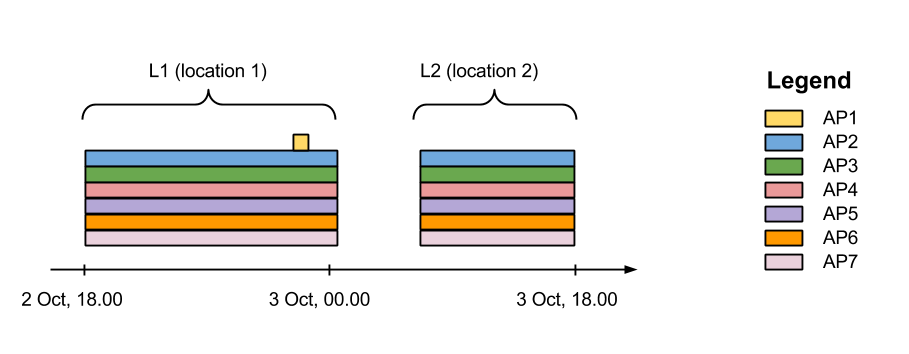
\includegraphics[height = 0.35\textwidth]{figures/isolated_ap.png}
\caption{Example of an isolated observable access point}
\label{isolated_ap}
\end{figure}

The above scenario considers a very small number of access points and a very
short period of time. The time gains in eliminating the access point which does
not provide so much information in this case would be very small. However, If we
are, for example, looking at a month of collected data for a user, we will have
entries for thousands of different access points that were observable at any
moment during this time. Out of these entries there can be hundreds of access
points which are never visible to the device during close scans and as such
their importance when determining the fingerprints for the different locations
is very limited, yet they do have a huge impact on the execution time needed to
actually extract the locations.

In order to solve this issue, we eliminate from the access points those ones who
are not respecting the following condition:
\begin{itemize}
  \item There is no time window of at least 5 minutes throughout the time
  duration of the analyzed data in which the access point has appeared for at
  least 5 times. %TODO - think about 5 times or 3 times and justify
\end{itemize}

% TODO - justify 5 minutes
We have chosen to use time windows of 5 minutes as we make the assumption that
any user will choose to spend minimum 5 minutes at each stop location. In case
the user spend less time, we can consider that they are just transitioning until
the next stop location.
                                  %Chapter 2
\chapter{Extracting locations from Wifi data}
\label{locations}
% 20 pages
Human mobility has been attracting a high degree of attention from numerous
study fields among which we find urban and traffic planning, traffic prediction,
the spreading of diseases and many others \cite{AsgariGB13} \cite{Brockmann08}.

The studies that have been conducted on this subject have been using various
ways to identify the travel behaviour of people. Some of them have focused on
studying the information gathered from observing the way in which money is
dispersed through time \cite{Brockmann06}, or they have been focusing in
studying the behaviour of mobile phone users by analyzing the way they move
based on the communication towers their phones are connecting to when they are
engaging in voice communication \cite{Barabasi08}. There are studies that try to
understand human mobility through the glass of social networks
\cite{yang2010using}, as it can be observed that individuals prefer to meet with
other people that are part of their community more often
\cite{Musolesi:2007:DMM:1317425.1317433}. GPS data has also been considered for
various studies \cite{cuttone2014inferring}, \cite{5657695}. The list of
elements that have been taken into consideration for trying to understand and
predict the way in which we are conducting our daily travels is far from being
short. 

\section{Wifi based positioning}

Even from the beginning of the 21st century, research has been actively
conducted for trying to use the Wifi system in order to determine real
positioning and different databases for positioning systems have been created.
These databases usually included the positions of the Wifi access points or RF
(radio-frequency) identified fingerprints \cite{Chen:2006:PMP:2166283.2166297}
\cite{Cheng:2005:ACM:1067170.1067195} \cite{Youssef:2005:HWL:1067170.1067193}
\cite{bahl2000radar}. Modern databases for Wifi positioning are created with
information about the signal strength for the Wifi access points and can
even have information about where they were discovered.

Koo et. al. \cite{koo2011autonomous} have explored an algorithm that can help
estimate the relative positions of access points corresponding to the real
geographic configuration with the help of multidimensional scaling techniques.
Considering the fact that access points are not able to tell real distances
between themselves and other access points, the study aims to estimate the
dissimilarities between different access points using scans. They have also
conducted an experiment in an office building in order to test the proposed
algorithm and the results showed an estimation error of approximately $7$ m.

Another study conducted in this similar direction is the one by Mok et. al.
\cite{mok2007location}. The authors explore the possibility of determining the
location of a device which can scan Wifi access points based on the signal
strength that the access points are displaying at the moment of the scan. They
estimate the positioning by performing a trilateration based on the information
the device gets from multiple access points. The accuracy for their algorithm
for the conditions that were present in their experiment was of about $1-3$ m.

Athanasiou et. al. \cite{athanasiou2009utilizing} give a very clear and
concrete description for two classes of wireless positioning systems. Their work
focuses on experimenting with parameters for these algorithms in order to find
the optimal solution in terms of accuracy under realistic settings. They also
adapt a global map matching algorithm in order to extract travel time maps from
wireless data and they propose a demonstration for showing that for high
sampling frequencies, the locations identified are comparable to the ones
derived from GPS data.

The two classes of algorithms that are explored by the authors are: centroid and
fingerprinting. \textit{Centroid} is presented as the fastest method for
positioning, however it depends on having the real location of the access
points. This information is in general unavailable and as such a proposed
solution is to estimate the locations of the access points by calculating an
arithmetic mean of all the coordinates at which it was visible. The
\textit{fingerprinting} method is based on the assumption that the access points
are stable over time (they do not change positions). This leads to the fact that
at any time, a measurement at a particular location will return the same list of
access points with the same signal strengths. As such, this list can be
considered as the unique fingerprint of the location.

% TODO add 2 figures for centroid and fingerprinting
Zhang et.al. \cite{zhang2012polaris} propose an algorithm based on
fingerprinting for estimating locations that takes into consideration the fact
that the signal strength from various access points does not necessarily stay
constant throught the time. They propose a way in which a similarity between
fingerprints can be calculated in order to determine if two fingerprints are in
fact representing the same location.

These are just a selection of works that have been conducted on finding a
solution for Wifi based positioning systems. With the growth and improvement of
Wifi systems, in time all barriers can be overcome and we could have a
positioning system that is as accurate yet considerably cheaper than GPS
positioning systems.

\section{Determining the fingerprint of a location}
In order to have a better understanding about the way in which the mobile phone
users have been moving throughout the experiment, we needed to have an image of
the way a given period of time would look based on their Wifi records from
SensibleDTU. As it has been presented in Section~\ref{data_structures}, the Wifi
data we are using for the present project consists in the following fields:
user id, timestamp, SSID, BSSID, RSSI and the context. However, considering the
amount of data involved, just by looking through the log files it is almost
impossible for us to understand at what moment the user might have reached a
location and when did they leave from it. In order to be able to do this, we
have created various visualizations considering different options, different
time frames and for multiple users in order to begin to understand what the data
can tell us, what can we use, what would we need and what can we discard when
moving further to defining what makes a location.

\subsection{Signal strength over time}

The first thing that we have tried to visualize was the access points (APs) that
were scanned by users' mobile phones throughout different periods of time. We
have plotted the APs and their registered signal strength for varied users in
order to see if we notice any patterns in their movements.

%userX == user 6
In Fig.~\ref{user_6_1d_lines} we can see how a day from the life of a random
user (referred to as userX) looks like. The day for which we have plotted the
data started on a Tuesday at $12:15$ pm and ends the next day right before the
same hour. The hourly intervals can be seen on the X axis, while the signal
strength values can be seen on the Y axis. The legend contains the top $10$ most
popular~\footnote{An AP is more popular than another in case it appears more
times during the period of time for which the Wifi scans are analyzed}

\begin{figure}[h]
\centering
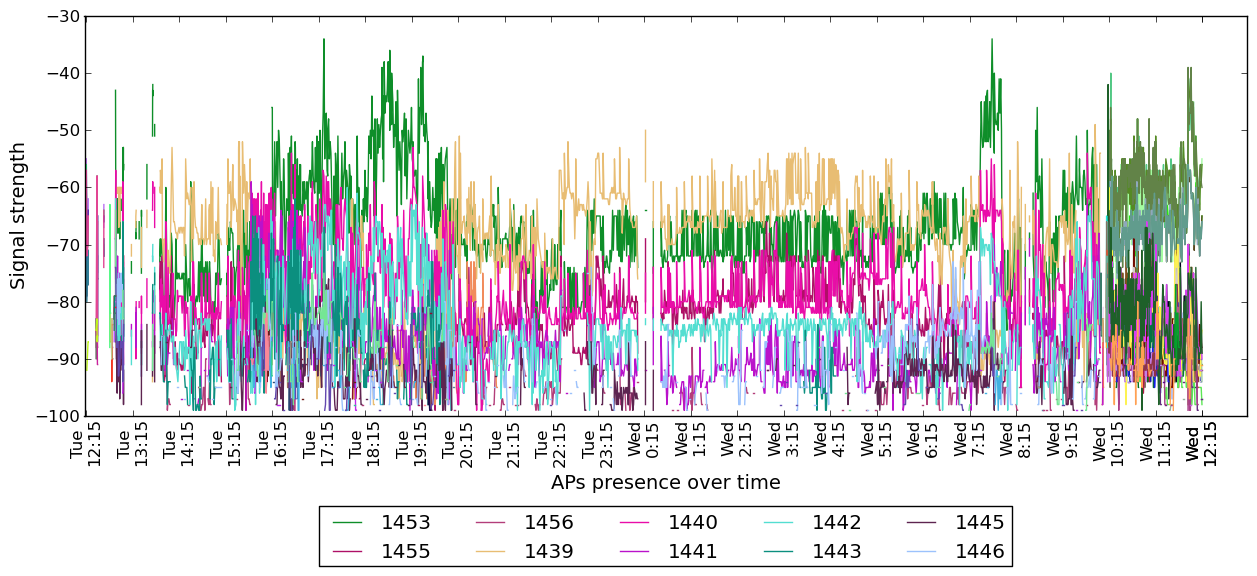
\includegraphics[width
=\textwidth, height =
0.4\textwidth]{figures/user_6_sorted_1days_plot.png}
\caption{Example of the APs registered for an user throughout one day (using
connecting lines markers)}
\label{user_6_1d_lines}
\end{figure}

The steps for creating this type of visualization are as follows:
\begin{itemize}
  \item Retrieve data for the time duration for which the visualization is made
  \item Keep track of all the timestamps at which each AP has been seen and the
  AP's signal strength at that moment
  \item In case an AP is scanned no more than $2$ minutes after a it was
  previously scanned, then a line can unite the two moments in order to mark
  their proximity. If the apparitions are more than $2$ minutes apart there is
  a high possibility that there has been a location change or that the AP is
  experiencing technical problems and as such has stopped being active.
\end{itemize}

Although we have tried to visualize this type of information in various ways
(using different types of markers), we found that this way is the easiest to
interpret by people. If we leave out the lines, for example, as it can be seen
in Fig.~\ref{user_6_1d_point}, it is quite hard to interpret where location
might start or stop.

\begin{figure}[h]
\centering
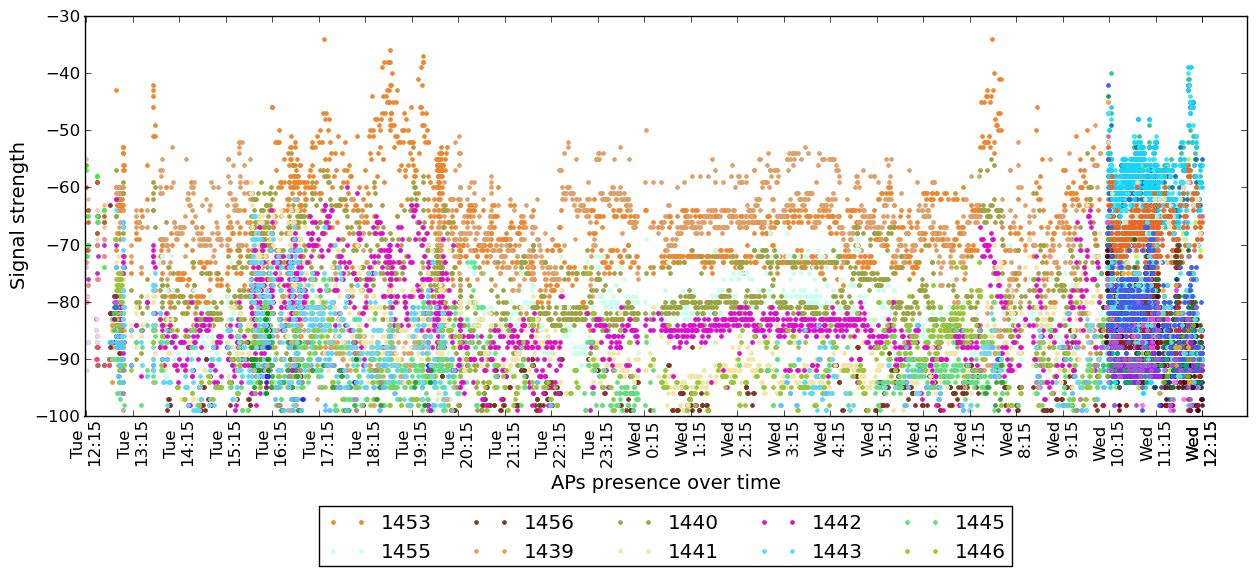
\includegraphics[width
=\textwidth, height =
0.4\textwidth]{figures/point_user_6_sorted_1days_plot.png}
\caption{Example of the APs registered for userX throughout one day (using
point markers)}
\label{user_6_1d_point}
\end{figure}

Other ways in which we have been experimenting with visualization for this can
be found in Appendix~\ref{appendix_signal_strength}.

By looking at Fig.~\ref{user_6_1d_lines} we are at some level able to
distinguish moments of time at which the user seems to be arriving at a
location~\footnote{For example, we can say that what we notice from Wednesday
at 10:15 until the same day at 12:15 is different than anything we can see
before that time so we can assume that it is a new location.}, however it is
hard to notice any patterns because we are only observing a single day in the
life of userX. 

% user Y = user 3
Let us look at the data gathered through $7$ days from another user's (referred
to as userY) life. The visualization for this data can be seen in
Fig.~\ref{user_3_7d}. The image gives out some very interesting information. We
can, for example, notice the repeating patterns which are dominated by the
orange, light green and blue colors. These patterns appear during the evening
and the night and we can assume that the user is spending this time at the
location which we can label ``home''.

We can notice some periods of time that are free. These free gaps like, for
example, from Monday morning until Monday evening are gaps in which no signal
was scanned and can mean that either the mobile phone was closed or that the
user decided to switch off the Wifi.

\begin{figure}[h]
\centering
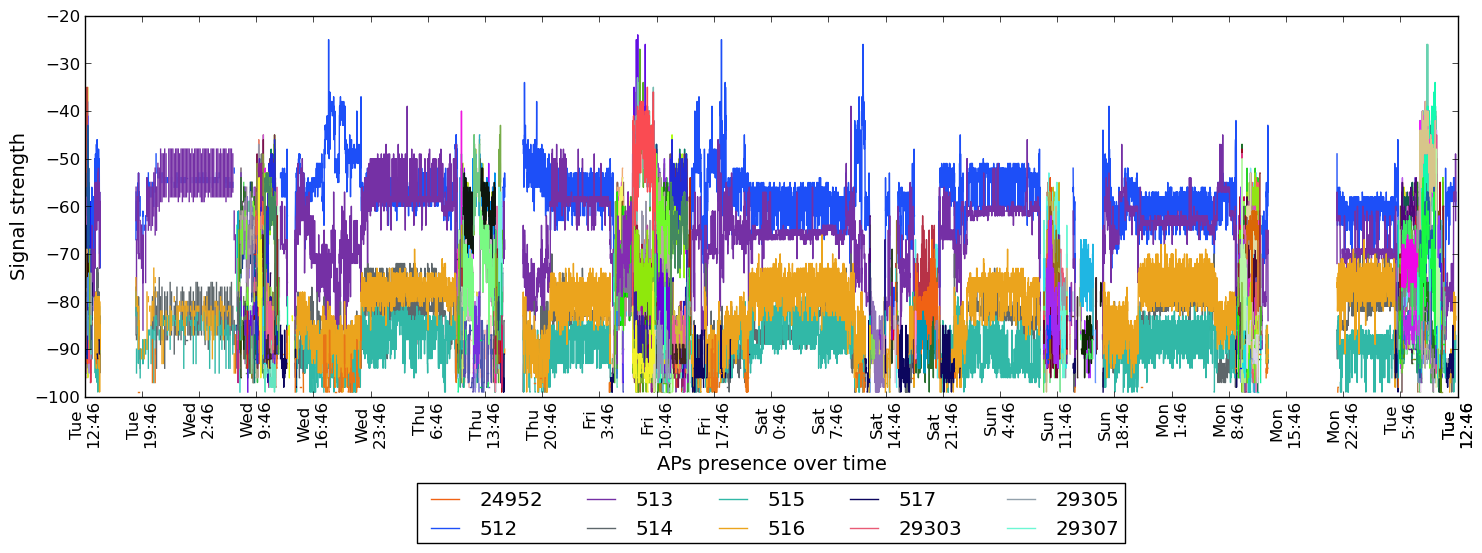
\includegraphics[width
=\textwidth, height =
0.4\textwidth]{figures/user_3_sorted_7days_plot.png}
\caption{Example of the APs registered for userY throughout 7 days}
\label{user_3_7d}
\end{figure}

We can also notice fragments in which the density of signals is quite high, for
example on Wednesday morning. This means that the user was located in a place
which has a large number of APs near and since we can notice a regularity in
this pattern we can assume that this place can be the University. This might
seem unlikely based on the fact that the patterns sometimes is identified during
the night, however this particular week is set in October when there are
deadlines for school projects that need to be handed in.

As we can see, these visualization can offer us a good first glance at what the
locations might be like, yet they also make us consider other things that we can
learn about the data. For example:
\begin{itemize}
  \item How many samples from each access point are received during a given time
  frame
  \item What is the average signal for various time frames for a given access
  point
  \item What are the running averages for signals from various access point
\end{itemize}
%As we can see, these visualization can offer us a good first glance at what the
%locations might be like, however, they also raise some interesting questions.
%For example:
%\begin{itemize}
%  \item Can the spikes in the signals cause any problems in determining
%  locations?
%  \item Does the sample density give us additional useful information for
%  extracting the locations?
%\end{itemize}

\subsection{Sample density}

When trying to identify locations based on the Wifi data, it is important to
only take into consideration the access points that actively contribute to the
fingerprint of the mentioned location. Before cleaning our data (as it has been
described in Section~\ref{data_cleaning}), isolated observable access points can
appear and unnecessarily burden the algorithm used for extracting the locations.
The best way to identify such access points is by analyzing the sample
density~\footnote{We define the sample density for an access point as the number
of times it appears in scans over a predefined time bin.} of the samples that
are identified during scanning.

In order to determine the sample density for each AP, we need to define a time
bin over which the sample density needs to be calculated. We have calculated the
density considering a time bin of $5$ minutes as we can assume that this amount
of time can be considered the minimum duration for which a user needs to be
situated in approximately the same place in order for us to not consider that
the location is a transition instead of a stop location.% TODO verify
% supposition

%TODO - userZ is 6 - 1 day , day 1
In Fig.~\ref{rssi_6_2nd_day} we have the different APs and their RSSI values at
the different moments when the mobile phone has identified them in the scans for
userX during the second day of observations. In Fig.~\ref{samples_6_2nd_day} we
can observe the sample density for one of the APs that are predominant during the visualized
time frame. As we can see, the number of times the AP is present in the scans
throughout the day is quite high and it is registered during numerous different
periods during the day. We can easily assume that this AP is one of the key APs
that define one of the locations the user has been associated with.

\begin{figure}[h]
\centering
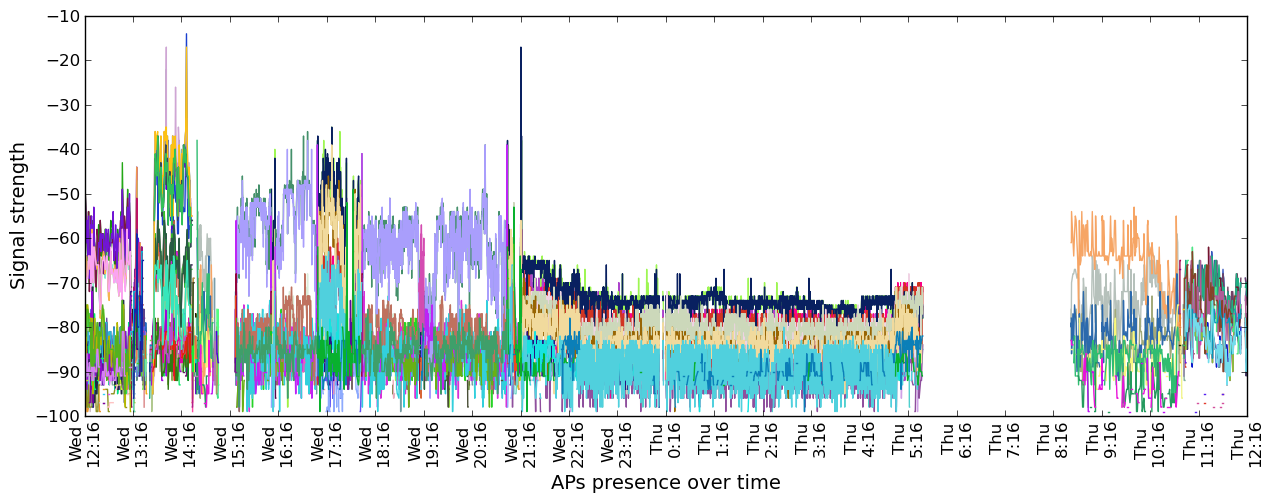
\includegraphics[width
=\textwidth, height =
0.4\textwidth]{figures/combinations/user_6_sorted_1days_plot_croped.png}
\caption{Example of the APs registered for userX throughout day 2}
\label{rssi_6_2nd_day}
\end{figure}

\begin{figure}[h]
\centering
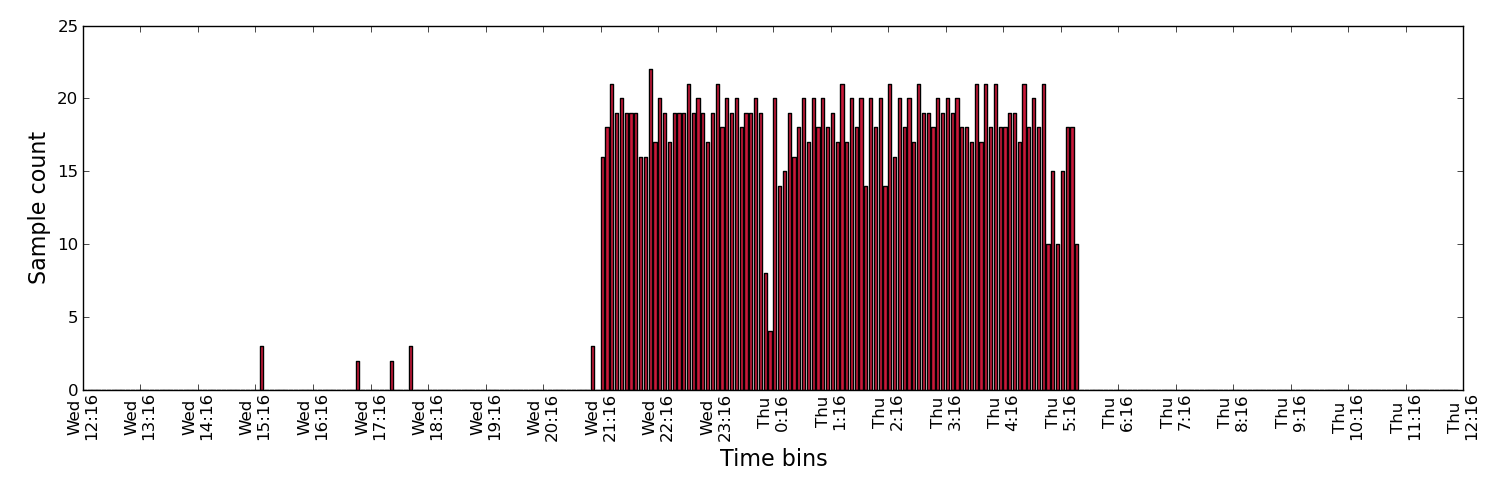
\includegraphics[width
=\textwidth, height =
0.4\textwidth]{figures/combinations/user_6_sorted_1days_plot_14280_histo.png}
\caption{Example of an AP which appears often}
\label{samples_6_2nd_day}
\end{figure}

On the opposite end as number of times it has appeared during the scans, we have
the AP in Fig.~\ref{few_samples_6_2nd_day}. As it can be seen, this AP only
appears $5$ times over a one single $5$ minute time bin. We can easily presume
that the presence or absence of this particular AP will not offer us relevant
information over the location at which the user was situated when it appeared in
the scans. This statement is also sustained by the fact that the user location
seems to be consisted from Wednesday $12:16$ up until around $13:16$ according
to what we can observe in Fig.~\ref{rssi_6_2nd_day}, even though the AP does not appear
throughout most of this time.

\begin{figure}[h]
\centering
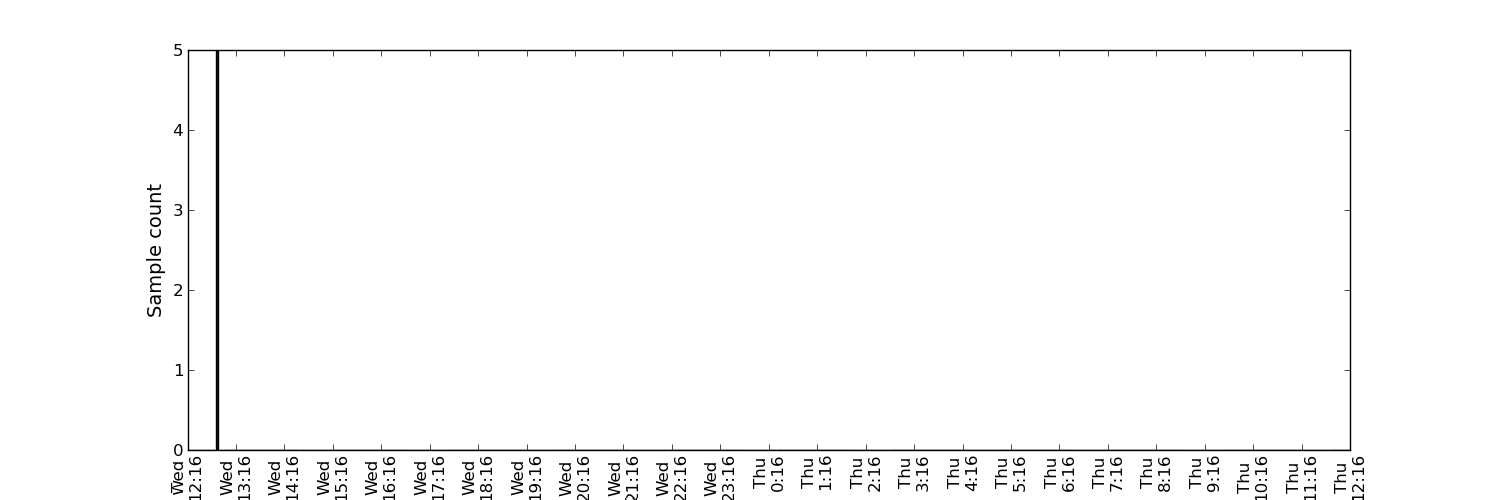
\includegraphics[width
=\textwidth, height =
0.4\textwidth]{figures/combinations/1553_modif.png}
\caption{Example of an AP that appears just a few times}
\label{few_samples_6_2nd_day}
\end{figure}

Other examples of visualizations for APs based on their sample density can be
found in Appendix~\ref{appendix_sample_density}% TODO - add stuff to appendix
% TODO - modify and add fig with only one apparitions with 5 samples in 5
% minutes -> to modify and say we take into consideration only those with more
% than 5 samples in 5 minutes

\subsection{Exploring the implications of the signal strength}
Something that is often taken into consideration during studies regarding the
determination of locations based on Wifi data is the value which indicates
the signal strength received from the various APs. The level of the signal
strength indicator can, in general, give us a good approximation of how close we
are to a particular AP. However, Wifi networks are susceptible to interferences
\cite{MahantiCWA10}, meaning that there numerous factors which can cause signals
to spike even in case the device which scans the region for AP signals does not
move. This can represent a factor of risk when including the signal strength
value in the location extraction from Wifi data as the same location could be,
at different times, be associated to an AP which has a signal strength that
oscillates based on other external factors.

In order to see if we can smooth down possible fluctuations we have employed two
mathematical tools. We have calculated the average signal strength, as well as
the running average, considering different length time bins.

\subsection{Average signal strength}
\label{average_sig}

In order to calculate the average signal strength of a given AP for a given time
bin, we needed to identify all the moments of time inside the given time bin in which
the AP has been spotted during the scans. The average signal of the AP is
calculated as the sum of all the strength values that have been recorded for the
AP inside the time bin and the sum is then divided to the number of recorded
apparitions of the AP. For example, if we were to have an AP which appears 6
times inside a $5$ minutes time bin with the following RSSI values [-60, -70,
-60, -80, -90, -60], then the average signal strength for this particular time
bin for our AP would be $avg = [(-60) + (-70) + (-60) + (-80) + (-90) +
(-60)] / 6= -70$ dBm.

We have calculated the average signal for various users and various days. We
have also calculated it for different time bin length. For example, for the same
data that we can see in Fig.~\ref{rssi_6_2nd_day} and for the same AP that has
the sample density represented in Fig.~\ref{samples_6_2nd_day}, if we visualize
the non-null averages calculated for time bins of $5$ minutes, we would have the
representation in Fig.~\ref{user_6_avg_1d_5m}. The X axis records the time
while on the Y axis records the values of the averages

% TODO plot only with this AP in normal mode and maybe make some observations.
%TODO add more to appendix.

\begin{figure}[h]
\centering
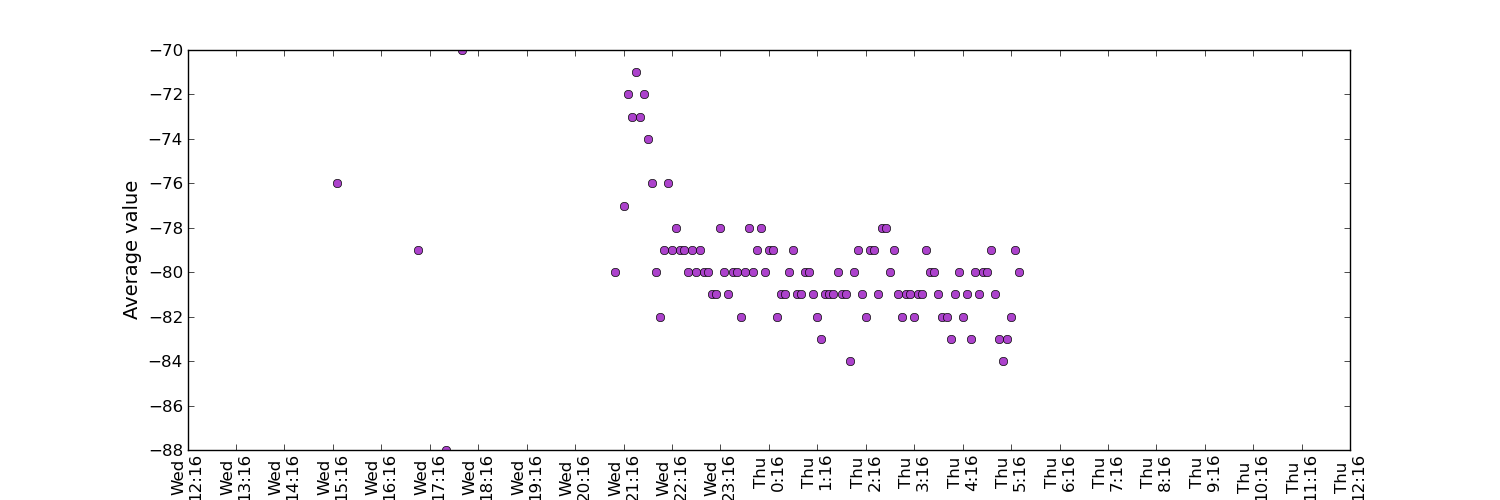
\includegraphics[width =\textwidth]{figures/combinations/user_6_sorted_1days_plot_14280_avg_sig.png}
\caption{Example of average signal strength visualization for userX}
\label{user_6_avg_1d_5m}
\end{figure}

The averages are represented by big dots symbols which appear at the beginning
of the time bin for which the average is calculated. For example, if we have
calculated an average for the interval $12:05 - 12:10$, the average is plotted
on the visualization at $12:05$. 

Additional examples of averages for different APs scanned during the same day by
userZ's mobile phone can be found in Appendix~\ref{appendix_signal_strength}.

\subsection{Running average signal strength}
\label{running_avg}
The average signal brings a small improvement as far as eliminating the signal
spikes go, however, an even better way in order to smooth out any signal
fluctuations is to calculate the running average\footnote{Also referred to as
the moving average} \cite{Hyndman09movingaverages}.

We have calculated the running average for different users and time frames, and
we have taken into consideration different time bins when calculating it.
The algorithm for calculating it is as follows:
\begin{itemize}
  \item For the selected user and the selected time frame, we have extracted for
  each AP the time stamps at which it has been identified by the user's phone
  \item We have divided for each AP the previously mentioned time stamps into
  bins of $2$, $5$ or $10$ minutes recording also the signal
  strength identified at each time stamp\footnote{By doing this we have the
  signal strength for the given AP at any moments it has appeared inside the time bin}
  \item The above identified time bins are overlapping. For example, if a
  sequence of signals $[-60, -80, -70, -70]$ that have each been identified at $1$ minute
  apart is to be divided into bins of $2$ minutes, the resulting $2$
  minute bins would be: $[-60, -80]$, $[-80, -70]$, $[-70, -70]$
  \item The running average is calculated as the sum of the values present in a
  time bin which is then divided to the number of values. For example, for the
  above time bins, the running averages would be $-70$, $-75$ and $-70$
\end{itemize}

In Fig.~\ref{user_1_APs_1d} we can see the APs associated with another user
(referred to as userT) and their signal strengths over a day.
Fig.~\ref{user_1_AP85_1d} shows the signal strength for just one of the
identified APs. The average signal as is presented in Section~\ref{average_sig}
for the same AP can be seen in Fig.~\ref{user_1_AP85_avg_1d}.
Fig.~\ref{user_1_AP85_rn2avg_1d}, Fig.~\ref{user_1_AP85_rn5avg_1d} and
Fig.~\ref{user_1_AP85_rn10avg_1d} present the running averages calculated for
the same AP for time bins of $2$, $5$ and $10$ minutes~\footnote{In this
representation, only the non-null values for running averages are displayed}.
The X axis of these figures track the succession of time moments while the Y
axis keeps track of the value of the running average calculated over this time.

\begin{figure}[!h]
\centering
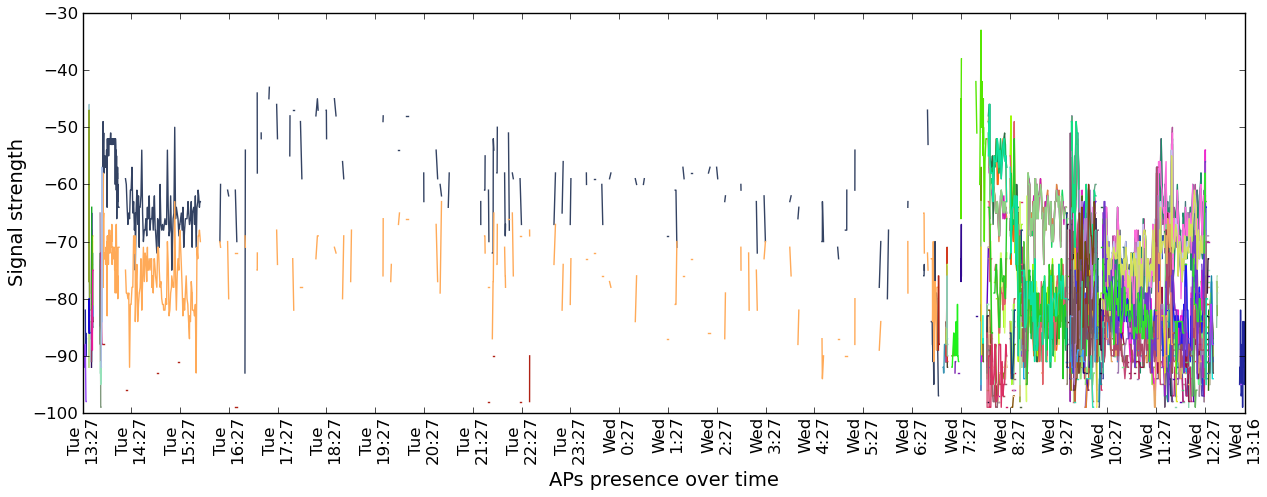
\includegraphics[width
=\textwidth, height =
0.4\textwidth]{figures/rn_avg/user_1_sorted_1days_plot.png}
\caption{Example of APs presence over time for userT}
\label{user_1_APs_1d}
\end{figure}

\begin{figure}[!h]
\centering
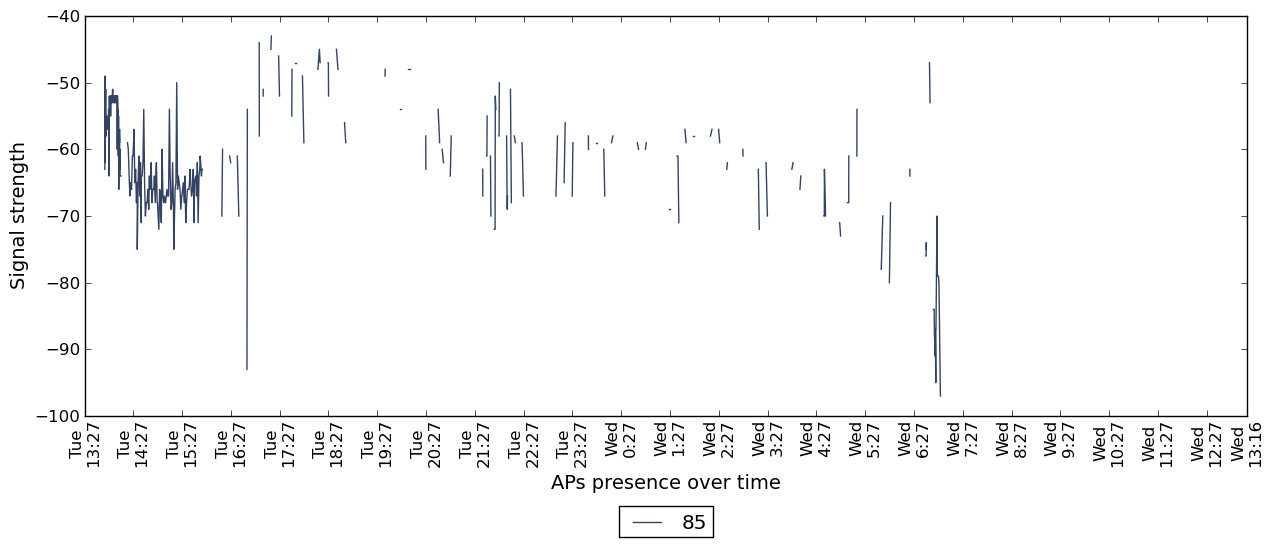
\includegraphics[width
=\textwidth, height =
0.4\textwidth]{figures/rn_avg/user_1_sorted_85_plot.png}
\caption{AP 85 for userT during 1 day}
\label{user_1_AP85_1d}
\end{figure}

\begin{figure}[!h]
\centering
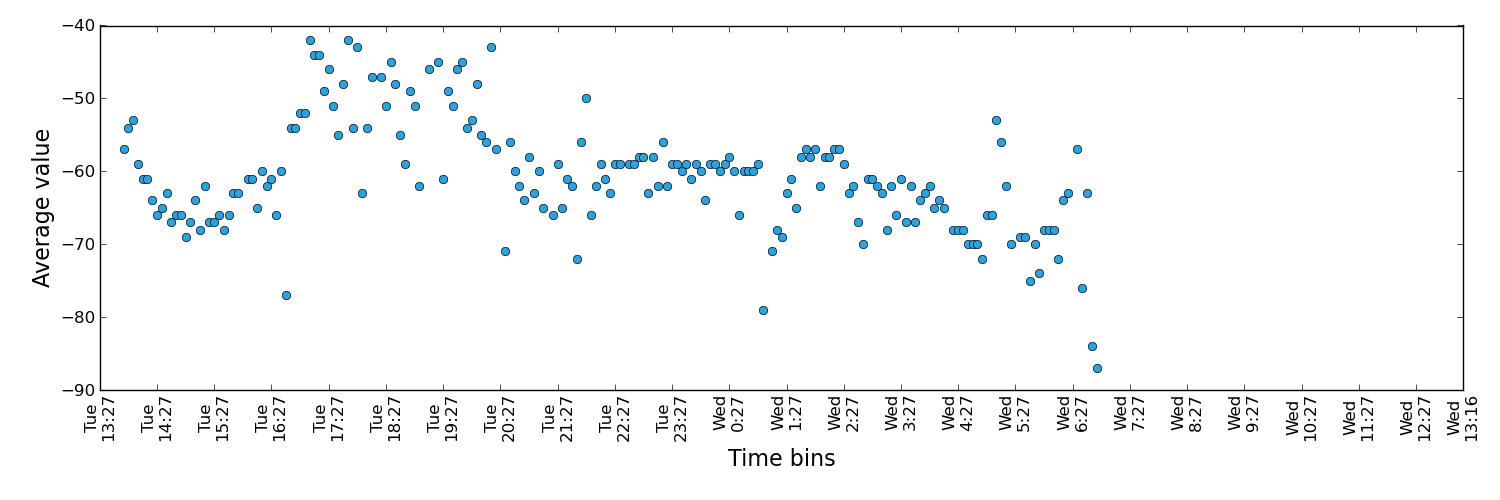
\includegraphics[width
=\textwidth, height =
0.4\textwidth]{figures/rn_avg/user_1_sorted_1days_plot_85_avg_sig.png}
\caption{Average strength for AP 85 for userT during 1 day}
\label{user_1_AP85_avg_1d}
\end{figure}

\begin{figure}[!h]
\centering
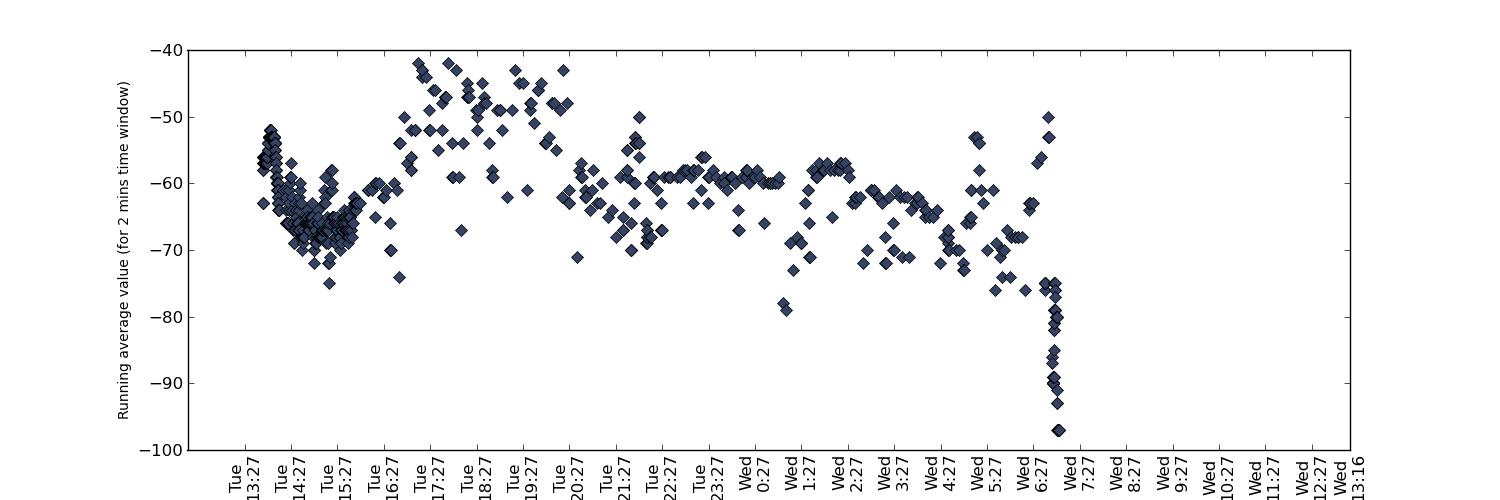
\includegraphics[width
=\textwidth, height =
0.4\textwidth]{figures/rn_avg/user_1_sorted_1days_plot_85_rn_avg_sig_2.png}
\caption{Running average for AP 85 for userT during 1 day (2 minute time bins)}
\label{user_1_AP85_rn2avg_1d}
\end{figure}

\begin{figure}[!h]
\centering
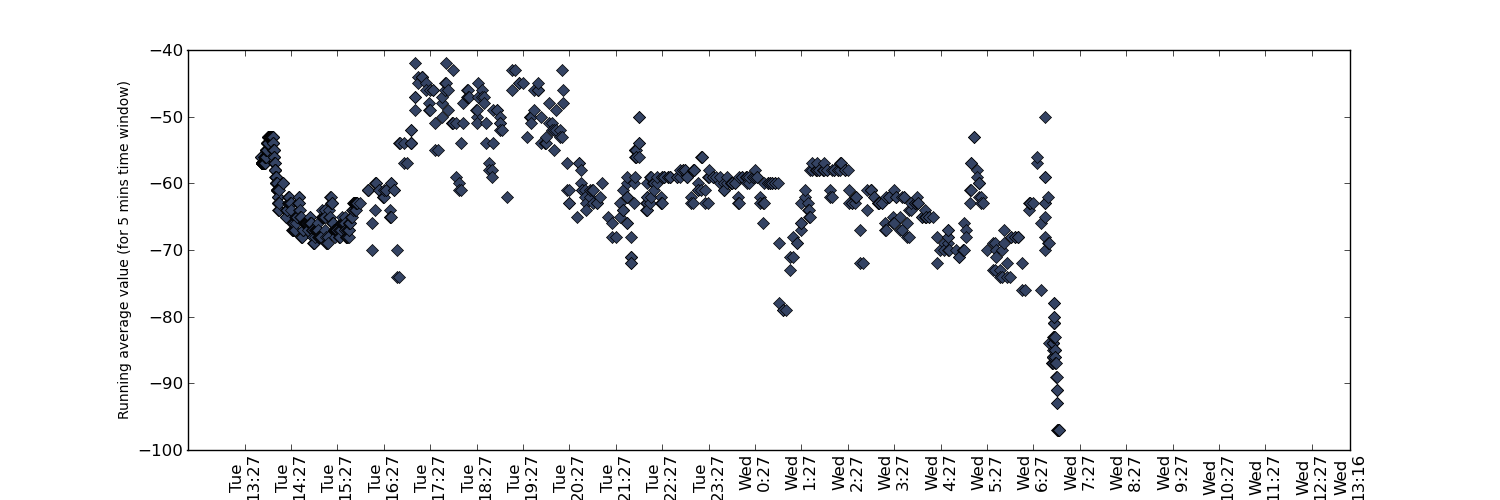
\includegraphics[width
=\textwidth, height =
0.4\textwidth]{figures/rn_avg/user_1_sorted_1days_plot_85_rn_avg_sig_5.png}
\caption{Running average for AP 85 for userT during 1 day (5 minute time bins)}
\label{user_1_AP85_rn5avg_1d}
\end{figure}

\begin{figure}[!h]
\centering
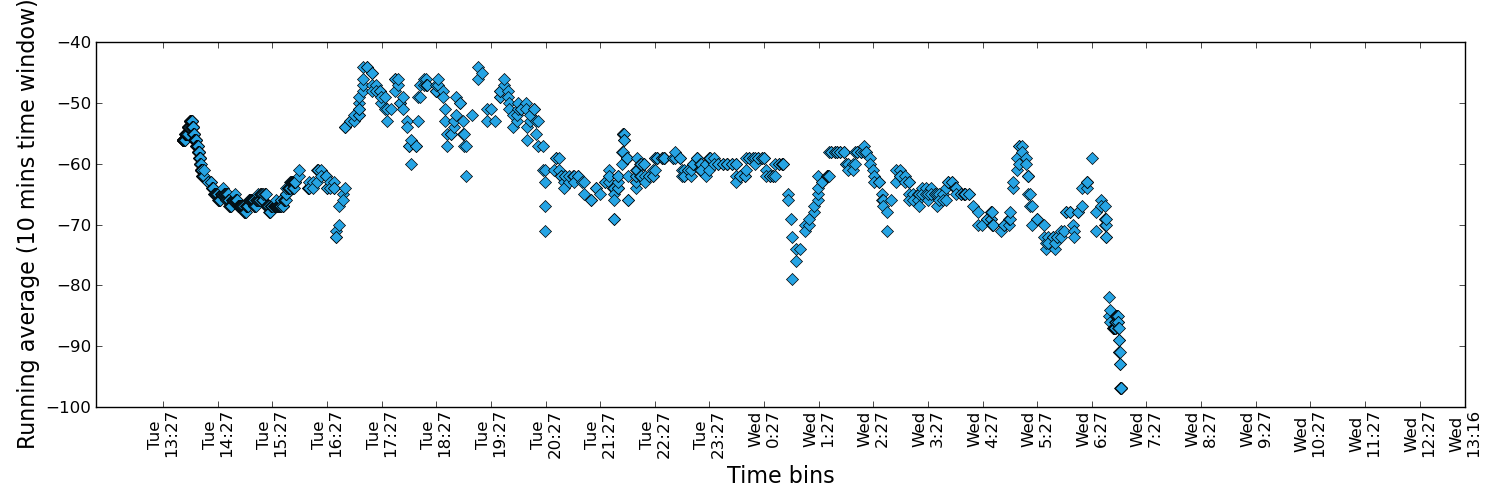
\includegraphics[width
=\textwidth, height =
0.4\textwidth]{figures/rn_avg/user_1_sorted_1days_plot_85_rn_avg_sig_10.png}
\caption{Running average for AP 85 for userT during 1 day (10 minute time bins)}
\label{user_1_AP85_rn10avg_1d}
\end{figure}

The way in which the fluctuations are smoothed down can be easily seen in the
figures that present the running averages calculated for various time bins. The
fluctuations are smoother as the time bin is increased.

Visualizations for running averages calculated for other APs identified during
the same day for userT can be found in Appendix~\ref{appendix_rn_avg}.

\subsection{Signal presence}
\label{sig_pres}

Even though averaging the signal strength through time improves at a certain
level the fluctuations in the signal strength, in a real environment spikes will
always be present and this will bring extra difficulties in estimating locations
based on fingerprints that contain the value of the signal strength for the
involved APs.

Another way of looking at locations is by calculating their fingerprint based
only on the identity of the APs that have been identified while the user was
found at that particular location. Basically, instead of defining a location
based on both the identity of the APs present and their signal strength, we
would only associate locations to visible APs.

The idea is simple and elegant and has been used in previous studies with
success \cite{Larsen:2009:MCT:1813042.1813063}. The concept behind is that, in
general\footnote{New APs can be set up or old ones can be changed with new ones
in time, which would mean a change in how the scans would look for the same
location. However, this is an issue that is outside the scope of the present
paper and work.}, at a given location the scans will always show the presence of
the same APs. If, after a time, the scans change and other APs appear, it is
reasonable to assume that the user has changed locations.

Since the information offered by the signal strength does not seem to be of the
ultimate importance, we can, in this case, try to identify the locations only
based on the presence of the APs. We consider that an AP is present at a
specific moment of time if the Wifi scans at that moment register a signal
strength from that AP. However, as it has been mentioned previously, due to
interferences, the signal from the AP might be lost for short periods of time
even when the user does not change their location.Considering this and the
assumption that, in general, people tend to spend at least a few minutes in a
stop location (otherwise meaning that they might be just transiting it), we have
made the decision to adapt for our case the definition for the presence of an
AP.

We divide our data into time bins of $5$ minutes~\footnote{We consider 5 minutes
as the minimum amount of time that needs to be spent in a location for it be
considered a stop location. This number can be easily adjusted in case further
research shows that it is not the optimal assumption.}. We redefine the presence
of an AP as follows: an AP is considered to be present for the duration of a $5$
minute time bin if it appeared in the scans at any point inside this time
interval.

We can use visualization in order to see how this transforms the way in which we
can understand the data. In Fig.~\ref{user_6_APs_2d} we have the different APs
that have been scanned throughout the duration of $2$ days for userX. In
Fig.~\ref{user_6_pres_2d} we can see the top $50$ predominant APs and their
presence over $5$ minutes time bin during the same $2$ days~\footnote{We
restrict our visualization to $50$ APs as it would be hard to understand an
image in which we would be displaying all the hundreds of APs which were
encountered throughout the $2$ days.}. The X axis keeps track of the time bins
throughout the $2$ days, while the Y axis represents the annonymized identifiers
for the APs.

\begin{figure}[!h]
\centering
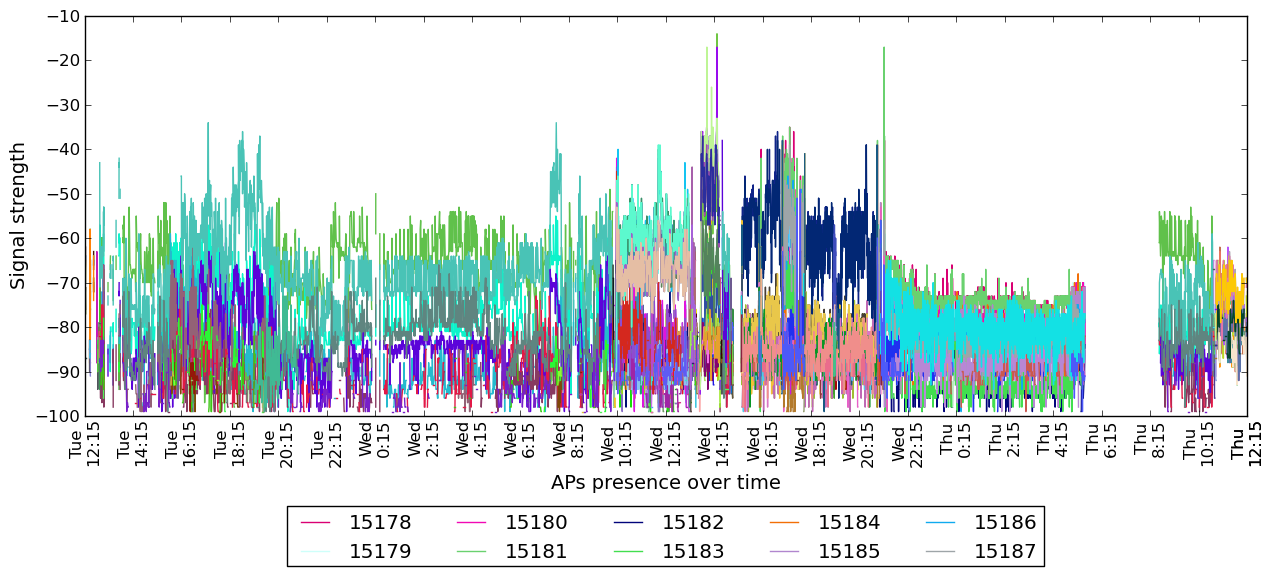
\includegraphics[width
=\textwidth]{figures/presence/user_6_sorted_2days_plot.png}
\caption{Scanned APs for userX throughout a duration of 2 days}
\label{user_6_APs_2d}
\end{figure}

\begin{figure}[!h]
\centering
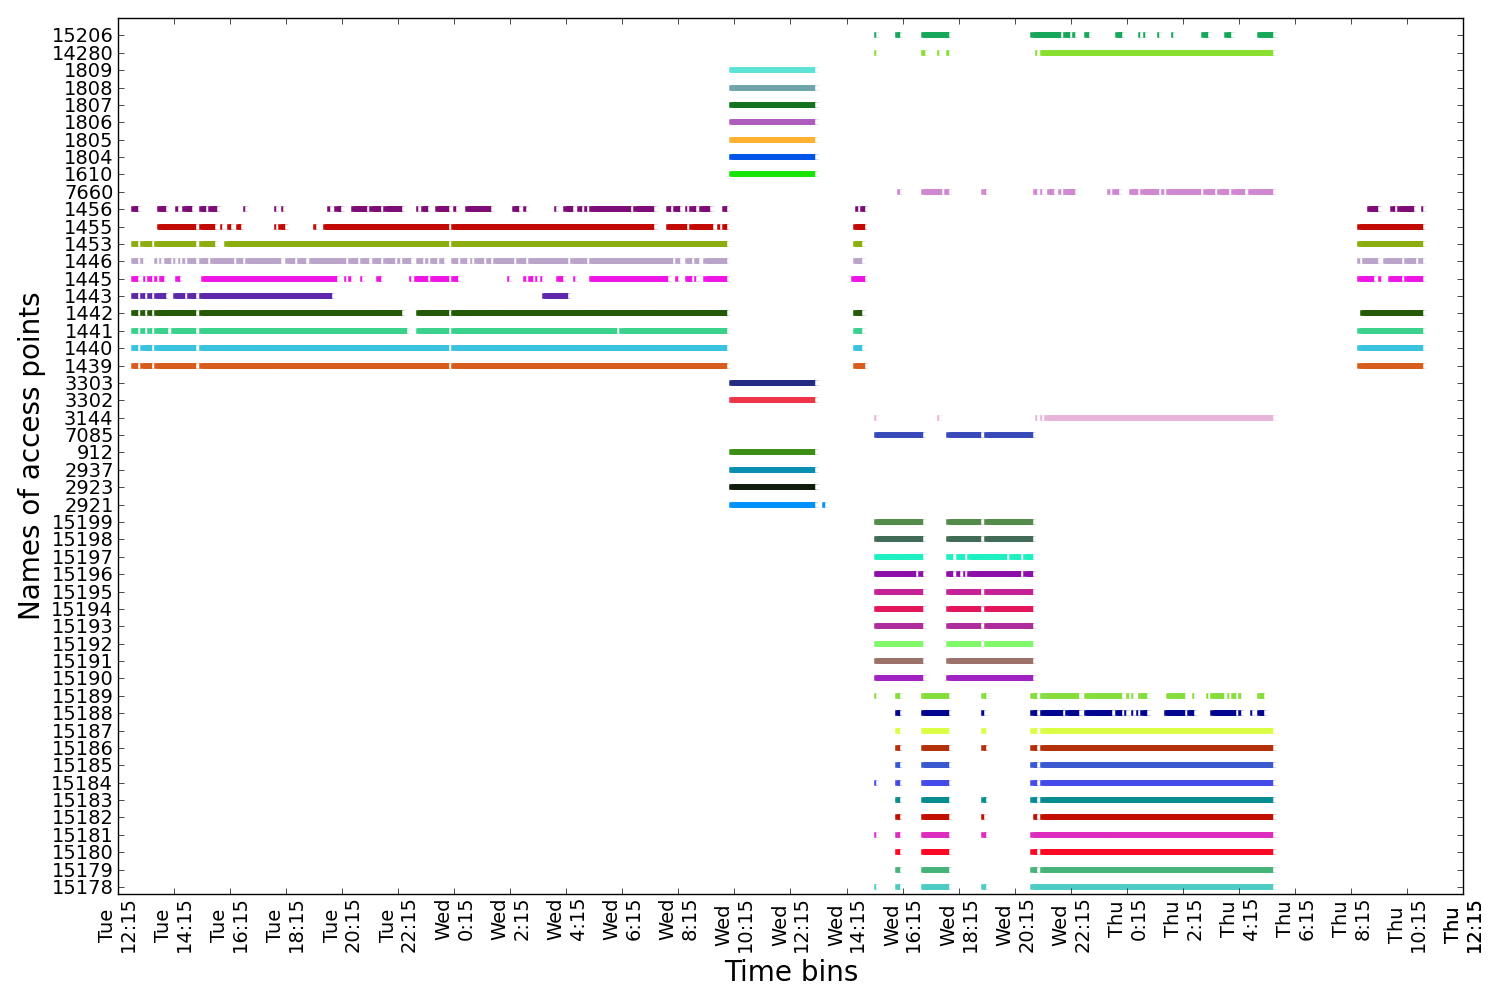
\includegraphics[width=1\textwidth]{figures/presence/user_6_sorted_2days_no_rssi_plot.png}
\caption{The most common 50 APs for userX during the given 2 days (presence
visualization calculated for 5 minutes time bins)}
\label{user_6_pres_2d}
\end{figure}

By closely observing the two visualization, it is quite easy to see that indeed
they are representations of the same period of time. Even if not all APs are
displayed in the visualization for the presence of the APs over time, we can
notice that, for example, the user has spent the time from Wednesday $21:15$
until almost Thursday $6:15$ in one location. This also coincides with what we
can observe in the visualization for all the APs (with signal strength) scanned
throughout this time.

In Appendix~\ref{appendix_pres} can be found a visualization for the presence
of APs for a period of $2$ days for another user. The presence for APs is determined for $5$
minutes time bins over the $2$ days.

\section{Extracting locations}
\label{extracting_location}

By visualizing the Wifi data in the way presented in Section \ref{sig_pres}, we
can begin to see how locations seem to succeed each other throughout the days of
a particular user. However, it is important to be able to implement a solution
that will extract these locations from a large amount of data so that we would
not be needed to examine the data manually. We have used different methods in
order to get the best possible approximation for identifying the locations. The
methods we have tried are: using \textit{networks}, using \textit{k-means
clustering} and using \textit{Hidden Markov Models}.

Before describing each of these methods, we have to clarify what we consider a
fingerprint of a location at a given time. A fingerprint of a location is
calculated based on the AP presence inside $5$ minutes time bins
(Section~\ref{sig_pres}) as follows:
\begin{itemize}
  \item We extract the data we want to analyze from the user (either for 1, 2
  or more days).
  \item We identify the APs from the data
  \item We divide the data into 5 minute time bins
  \item For each time bin we identify the APs which have been spotted during the
  $5$ minutes and we attribute them the value of 1 (meaning that they are
  visible to the mobile device during that time bin); the remaining APs will
  have attributed the value 0 (not visible) for the given time bin.
  \item Each fingerprint describes a time bin and shows what APs were visible
  during it and which are not
\end{itemize}
for consecutive $5$ minutes time bins.
The fingerprint contains the names for all the APs which are associated to the user throughout the time
frame we are analyzing (e.g. 1 day, 5 days etc.) and each AP has associated to
it a value which represents its presence throughout the $5$ minutes 

\subsection{Network theory}

Networks have a high degree of importance when trying to understand human or
animal behaviour. They have been used in combination with social platforms in
order to extract a new definition of friendship \cite{cho2011friendship}, they
have been used for monitoring animal behaviour \cite{4116628}, or to understand
the economical situations cause by the way in which people interact
\cite{Copic05identifyingcommunity}, or just to understand underlying communities
of people. During our research, we have considered the use of network theory in
order to extract locations from Wifi data.

In theory, we can expect that the APs that are identified at a particular
location will not appear in the scans the user's phone will have from another
location. This assumption is sound as the APs will rarely be moved and as such
they should always be associated to the same place. In this case, we should
expect that the succession of locations can be similar to what we can see in
Fig.~\ref{user_6_tn}., where AP1-AP6 are associated to location number 1, while
the remaining APs are associated with location 2 and the APs never overlap.

\begin{figure}[!h]
\centering
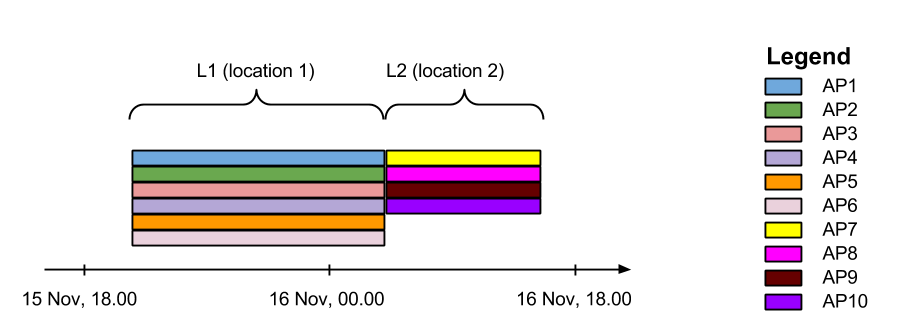
\includegraphics[width=1\textwidth]{figures/networks/theoretical_network.png}
\caption{Example of how, in theory, locations should be displayed through the
presence of APs}
\label{user_6_tn}
\end{figure}

The idea behind constructing the network  that can be used to extract the
locations is simple. A graph can be created for each user from their data and
the locations can be identified as follows:
\begin{itemize}
  \item We consider each found AP from the user data as a node in the created
  graph
  \item We construct a presence matrix for the identified APs. Each line in the
  presence matrix is associated to an AP and contains the signal presence
  (Section \ref{sig_pres}) calculated for the AP considering $5$ minute time bins
  throughout the time we are evaluating
  \item For each time bin, we identify the APs that are present trough it and
  we connect each two of them with an undirected edge (in case they have not
  been connected at a previous time)
  \item Since signal from various APs can be lost due to interferences, for each
  two APs for which we have created a connecting edge, we keep and update a
  variable which represents the number of times the APs have been identified in
  the same time bin
  \item After the network is completely created, we normalize the counts of how
  many times each two APs have been seen in the same time bin by dividing the
  counted value to the maximum number of apparitions of either of the two access points
  \item After the normalization we remove the weak links~\footnote{In this
  case, a link is considered weak if after normalization its associated value is
  below a given threshold}
  \item We consider the resulting connected components to be the extracted
  locations
\end{itemize}

An example on how to construct such a graph if given four APs and their
presence matrix can be seen in Fig.~\ref{network_calc_example}

\begin{figure}[!h]
\centering
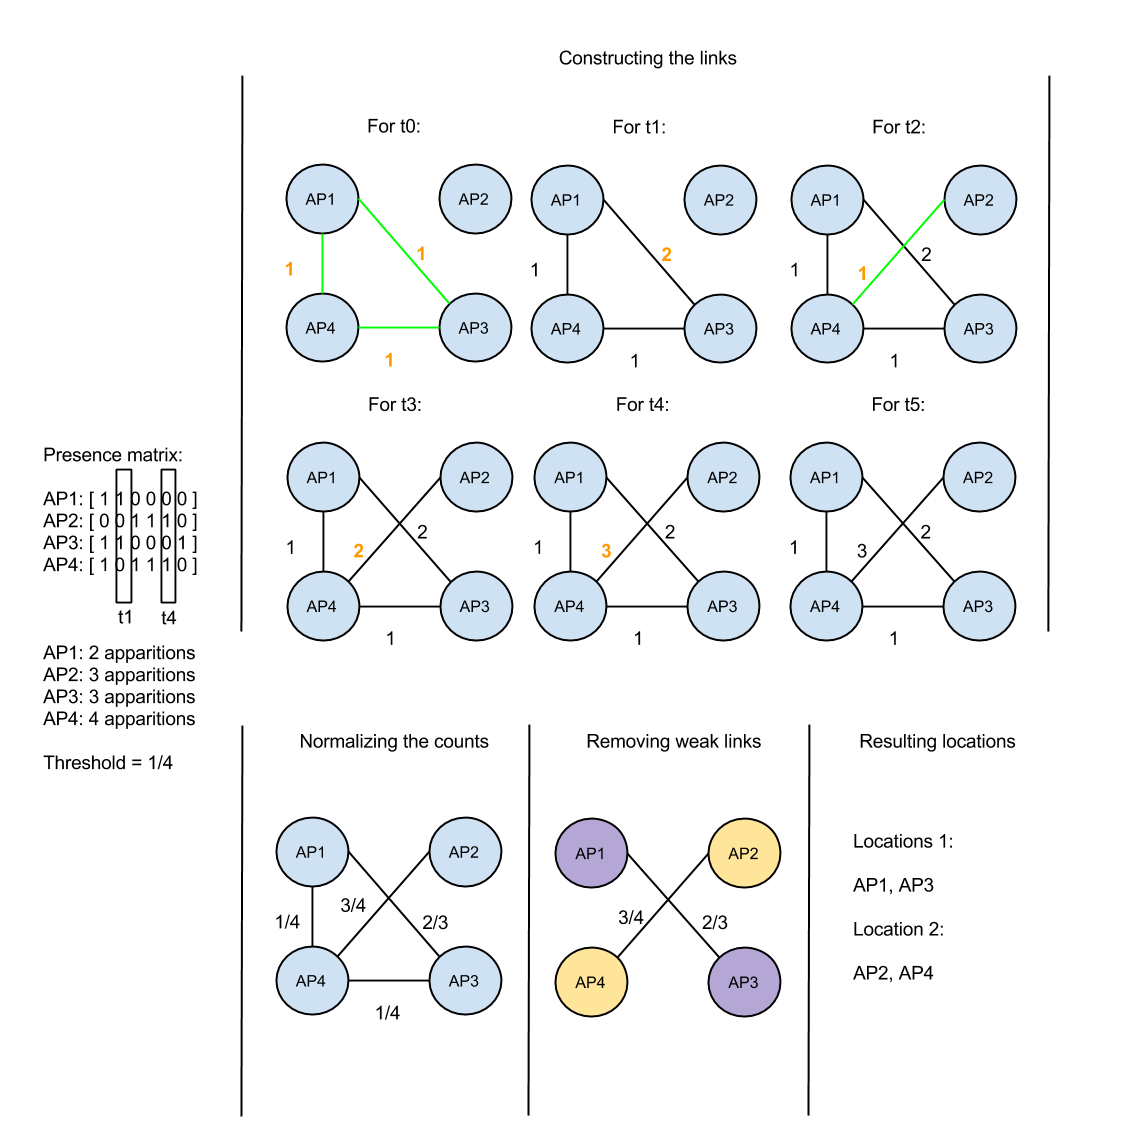
\includegraphics[width=1\textwidth]{figures/networks/net_constr_ex.png}
\caption{Example of constructing a network}
\label{network_calc_example}
\end{figure}

We have applied the previously described algorithm for a selection of users, but
the results have not been satisfactory.

For example, we can take data for one day for userX. The visualization for the
identified APs and their presence throughout this time can be observed in
Fig.~\ref{user_6_pres_1d}. By looking at this image, we can observe that the
user has been in f$2$ main locations during this day.

\begin{figure}[!h]
\centering
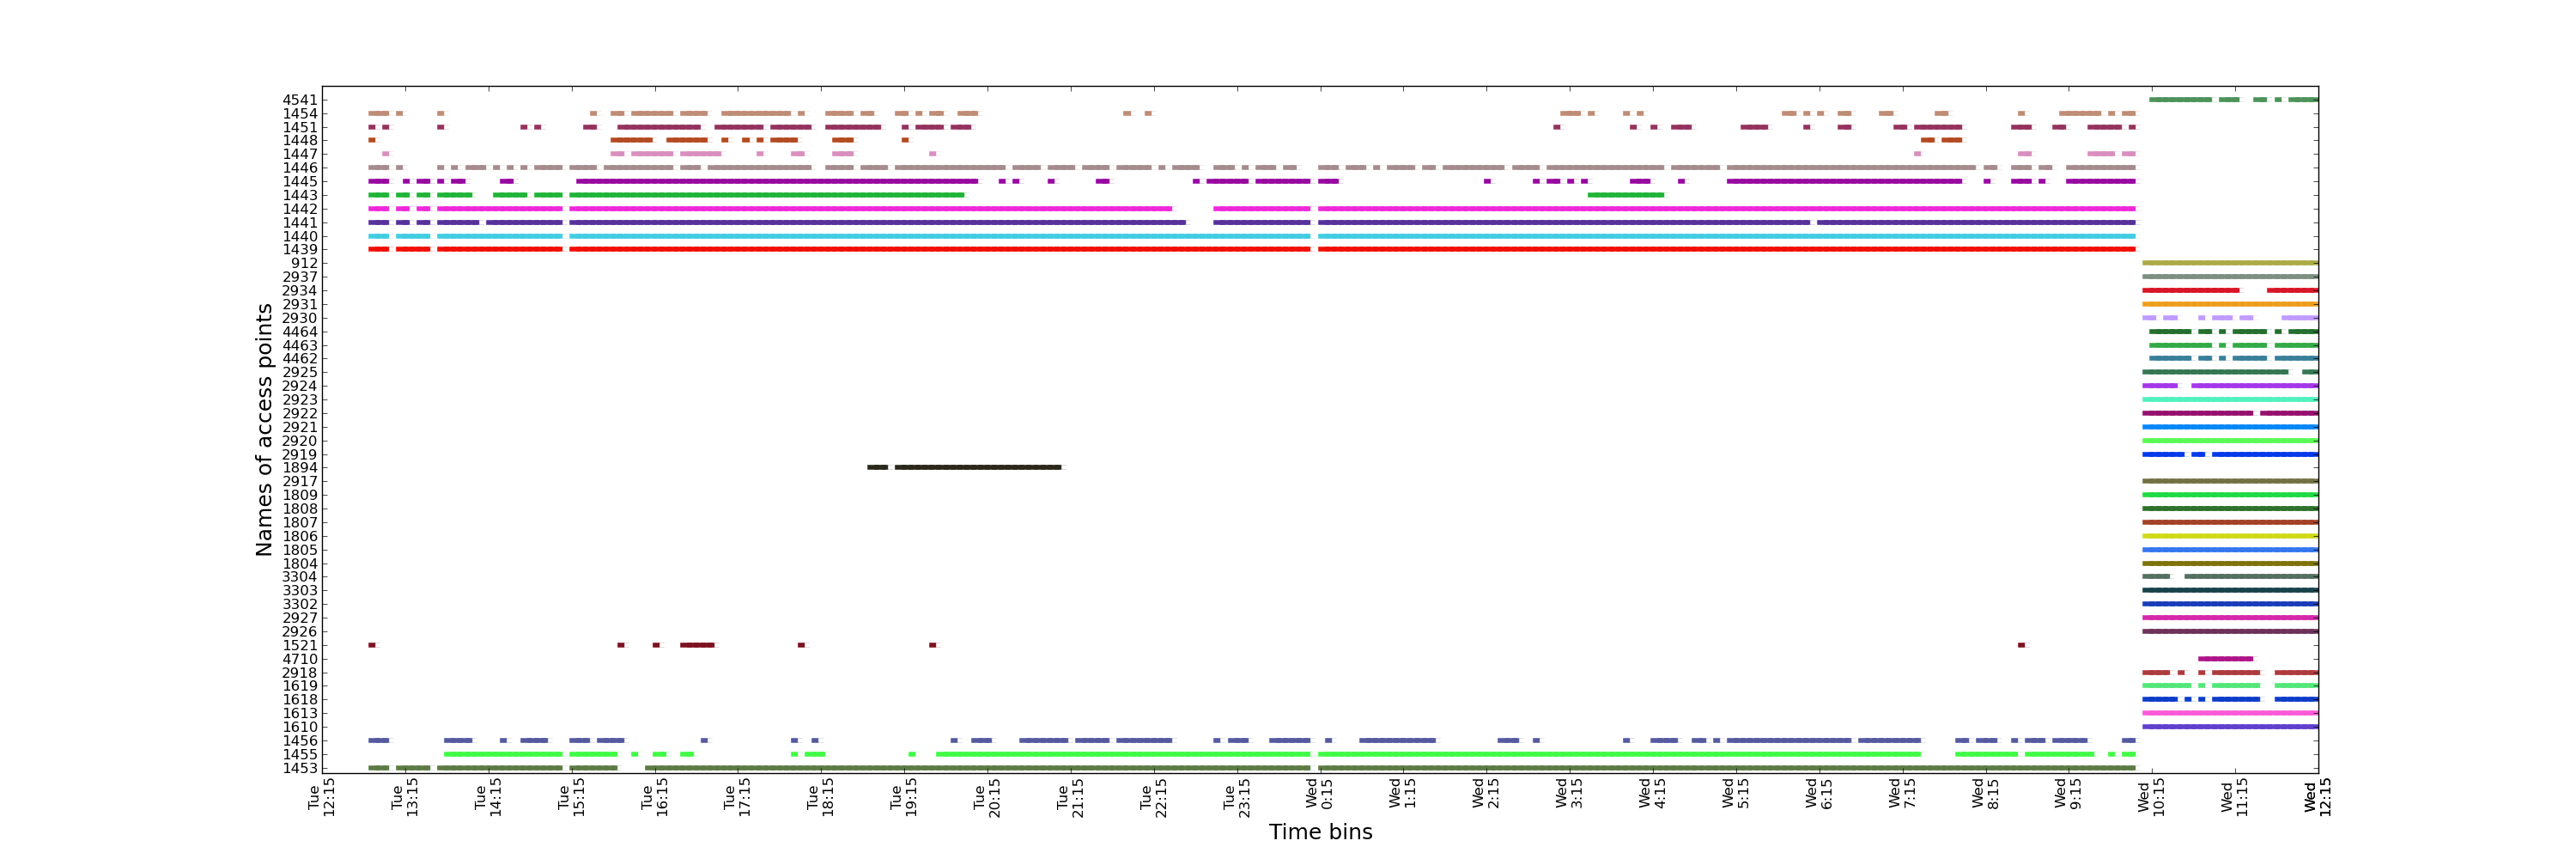
\includegraphics[width=\textwidth]{figures/networks/user_6_sorted_1days_no_rssi_plot.png}
\caption{The most common 50 APs for userX during one day scan records}
\label{user_6_pres_1d}
\end{figure}

When running the algorithm that extract the locations based on the constructed
network, we obtain $21$ connected components which have the potential of being
locations. The image for the connected components can be seen in
Fig.~\ref{user_6_networks_1d} 

\begin{figure}[!h]
\centering
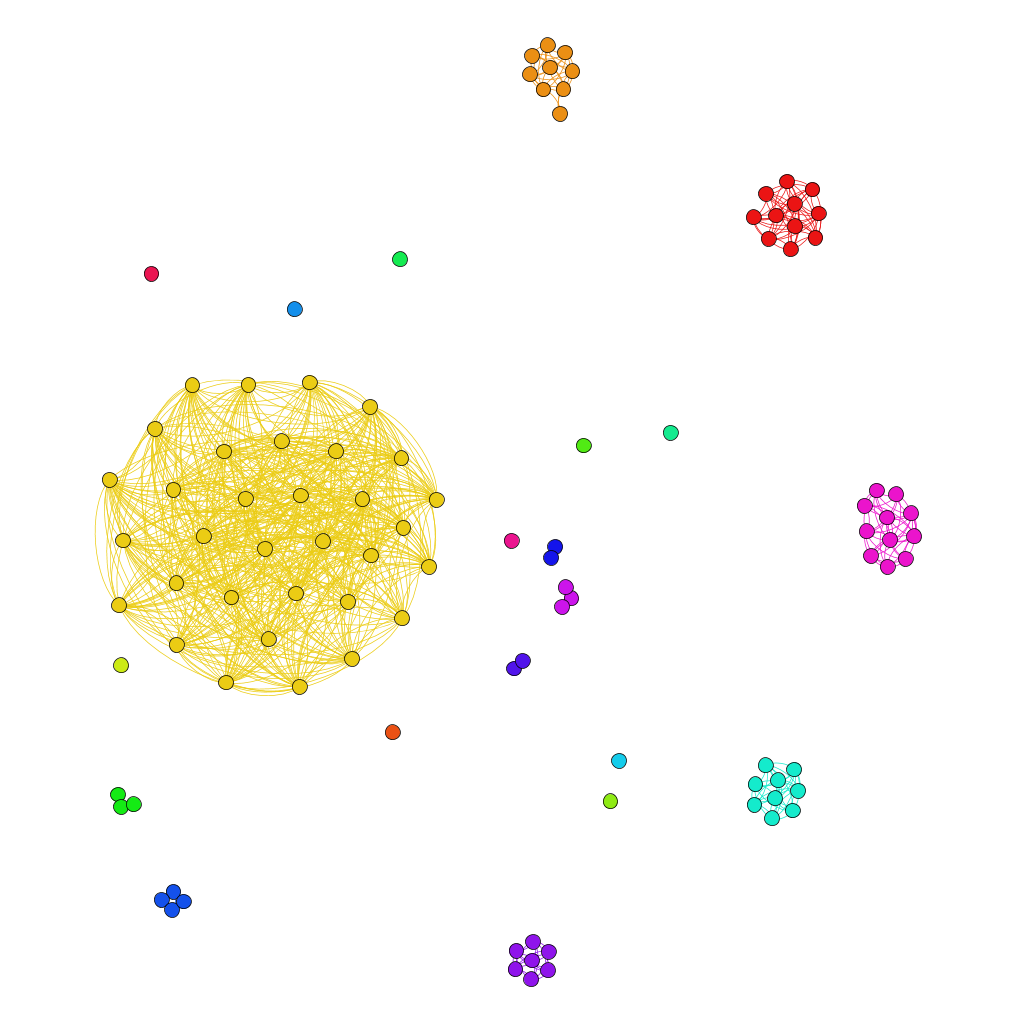
\includegraphics[width=0.7\textwidth]{figures/networks/user_6_day0_networks.png}
\caption{Locations identified with networks for userX during one day}
\label{user_6_networks_1d}
\end{figure}

We have tried to adjust the threshold for eliminating weak links yet the results
are in most cases unsatisfactory. Upon closer analysis we have observed that
this can be cause by the fact that, sometimes, there are a high number of APs
that even though they are in reality tied to a given location, their signal
fluctuates often and as such, the algorithm identifies them as part of a
different location and as such we have locations consisting in only a very small
number of APs that in reality could have been integrated in other locations.
This observation is sustained by the size distribution of the generated networks
(example for such a size distribution determined for the network in
Fig.~\ref{user_6_networks_1d} can be seen in
Fig.~\ref{user_6_size_distribution_1d}). Another thing we have observed is that
there are adjacent locations which can have interfering APs signals. This means
that our original supposition that, at all times, the APs that are visible from
a location will stop being visible in any other location does not always hold.

\begin{figure}[!h]
\centering
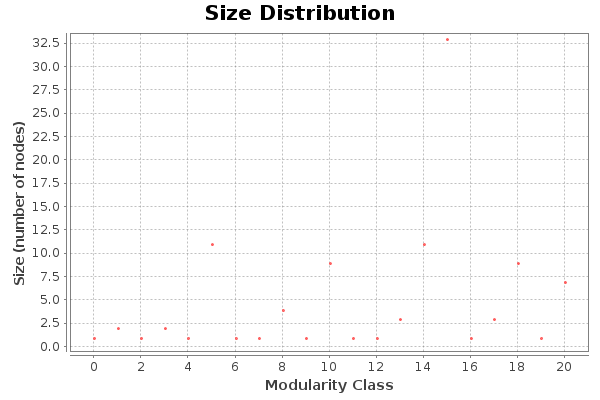
\includegraphics[width=0.7\textwidth]{figures/networks/communities-size-distribution.png}
\caption{Size distribution of locations based on the number of APs associated to
them }
\label{user_6_size_distribution_1d}
\end{figure}

%TODO cum ar arata efectiv locatiile fata de cum sunt
For generating the networks and the size distributions, we have been using
Gephi~\cite{Gephi}. For visualizing the visualization in
Fig.~\ref{user_6_networks_1d} we have used the Force Atlas $2$ layer which has
been configured in order to avoid overlapping of components.

\subsection{Cross validation}
\label{cross_valid}

For both the k-means and the Hidden Markove Models approaches on extracting
locations out of the user data we have been faced with a problem. The problem we
have been faced with is that both these algorithm need to know how many
locations they are trying to identify. However, we cannot know for sure, from
the beginning, how many locations a user has been visited during a given time.
In order for us to have a good estimation for the number of locations we could
be expecting to find inside a time frame, we have used the cross validation
technique, more specifically we have used the 10-fold cross validation method.

Cross validation \cite{Kohavi95astudy} is a technique for model validation that
tries to asses how the results given by a statistical analysis of some given
data can be generalized to an independent data set. The main use of cross
validation is in problems that deal with prediction. Prediction problems usually
deal with a set of training data and a set of testing data that the model needs
to be able to react to as expected.

The k-fold cross validation divides the data we have at our disposal in k equal
sized subsamples in a random way~\footnote{Random in this case means that
each of the subsamples contains elements from the original sample that are
most likly not in their original order.}. K-1 of the resulting subsamples are
used as training data, while the remaining subsample is used as testing data.
The samples are then rotated so as each of them becomes, in turn, testing
data while the others for the training data. The k results are then combined in
order to retrieve an unique estimation for the original data and an evaluation
of the accuracy of the prediction model can be done based on how close the
result is to the original data. The k value can be any number as long as the
data can be divided into k subsamples. A value that is oftenly used for k is 10
\cite{mclachlan2005analyzing}.

An example of how 2-fold cross validation works for four location fingerpints
can be seen in Fig.~\ref{2foldvalid}.

\begin{figure}[!h]
\centering
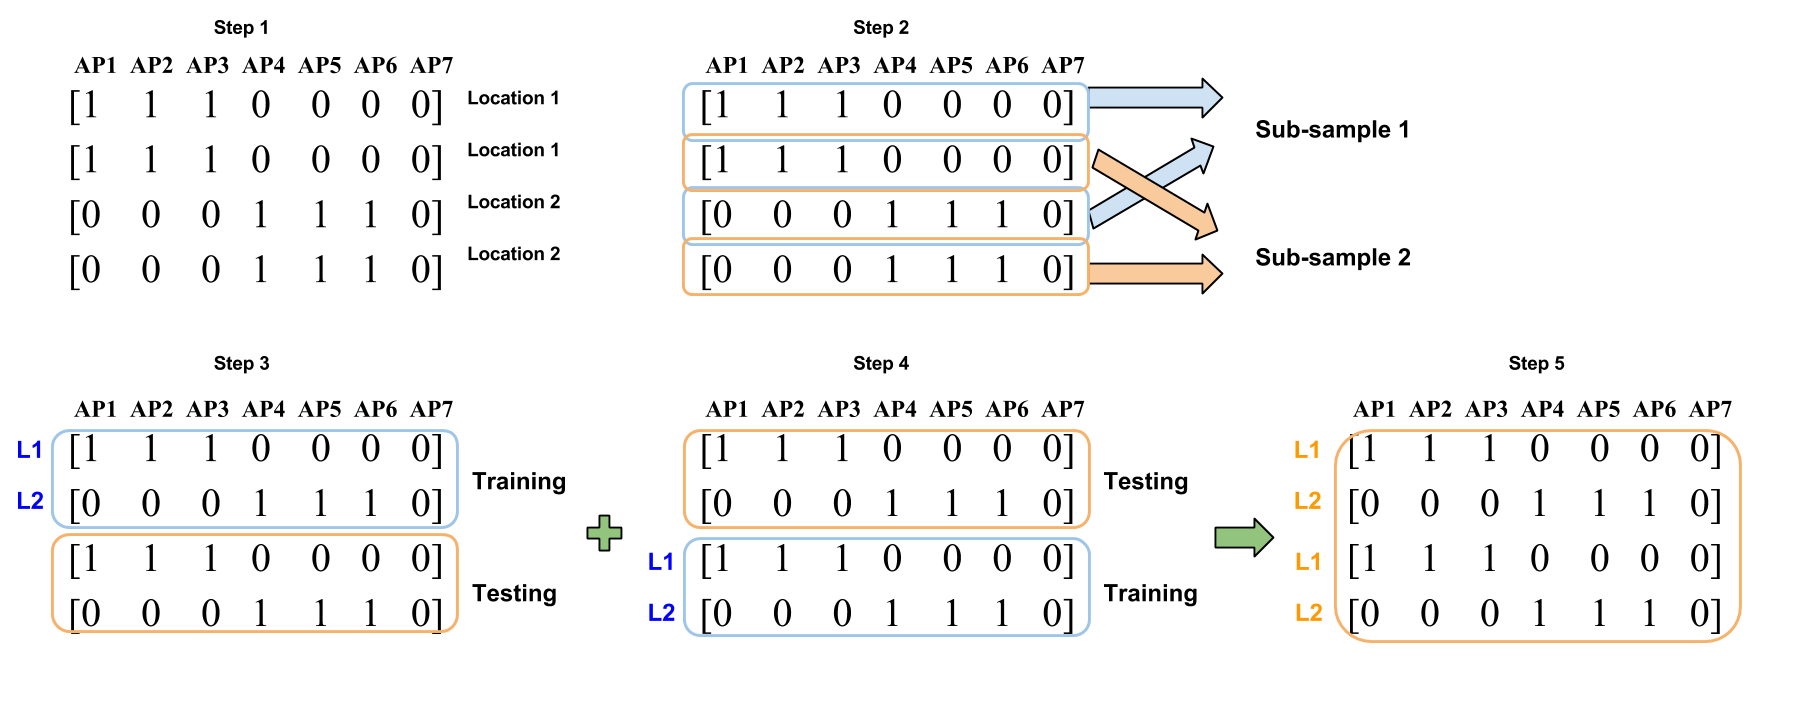
\includegraphics[width=\textwidth]{figures/kmeans/2-fold-validation.png}
\caption{Example for 2-fold cross validation}
\label{2foldvalid}
\end{figure}

In Step$1$ we have the four fingerprints. Let us consider that the algorithm
that we are using to extract the locations based on these fingerprints have
identified the location 1 and 2 as they can be seen in Step$1$. In order to see
if our algorithm behaved as expected, we can cross validate the result using in
this case a 2-fold cross validation. We are randomly selecting the $2$
subsamples as is seen in Step$2$. The blue color is associated with the training
data, while the orange color is associated with the testing data. In Step$3$ the
first subsample is treated as training data while in Step$4$ the second one
represents the training data. After the test data are classified based on the
training data we can combined the results into one single sample which is
presented in Step$5$. In this the cross validation has returned a result which
matches the original estimation made by our selected algorithm, which means that
the algorithm we have used has worked fine.

\subsection{K-means clustering}
\label{k-means}

The k-means algorithm is a popular method for analyzing clusters in data mining.
The first time the ``k-means'' term was used was by MacQueen
\cite{Macqueen67somemethods}, yet the standard algorithm for the k-means problem
was proposed by Lloyd \cite{Lloyd:2006:LSQ:2263356.2269955}. The idea behind
this algorithm is to start the clustering process by having k original groups of
only one point each. After this initial setup, each new point can be added to
the cluster that has the mean nearest to the new point. After a new point is
added to a group, the mean of the group is updated, and at each stage the k
means will represent the means of the k groups.

The Lloyd algorithm for k-means is the solution that is used for creating the
k-means tool by scikit-learn \cite{SL}. We have used the tool provided by
scikit-learn in order to try to extract the places where a user has been
situated at during a time frame based on the fingerprints that we can determine
for that time frame. Our goals was to use the k-means algorithm to cluster the
fingerprints that are similar enough as to be associated to the same location.
However, since we cannot know for sure the number of locations (clusters) we are
to expect for a given time frame, we are running the k-means algorithm with
different values for k and we perform 10-fold cross validation in order to see
what value has generate the most likely estimation.

The steps in extracting the locations with k-means and 10-fold cross validation
are as follow:
\begin{itemize}
  \item We select the time frame (number of days) for which we want to extract
  the locations
  \item We retrieve the data and extract the fingerprints
  \item Since previous research shows that in general people spend most of their
  time in a small amount of locations ($5$ to $50$) \cite{Barabasi08}, we choose
  the maximum number of locations we are expecting to find as the minimum value
  between $50$ and the rezult for the number of days multiplied by
  $10$\footnote{By observing the visualization for the presence of APs during
  different days in different users' life, we have observed that in general
  they seem to spend their time during a day in a most 10 locations}
  \item For each possible number for locations from between $2$ and our
  previously selected maximum we run the k-means clustering algorithm on the
  identified fingerprints
  \item The estimations are cross validated in order to see which number of
  locations has generated the optimal approximation for the given fingerprints
  \item In case more locations have generated equally good results we selected
  as number of expected locations the highest of them
  \item This algorithm is ran $10$ times leading to $10$ estimations for the
  number of locations. Out of these estimations the one which appears the most times
  out of the $10$ results is considered correct.
\end{itemize}

We ran the algorithm for $10$ times in order to ensure that we the final result
is as less influenced by the random fact involved in the determination of the
subsamples for the cross validation as possible. At the end of the algorith we
have the estimation for the locations throughout the selected time frame. An
example for such an estimation can be seen in Fig.~\ref{user_3_days1_2_kmeans},
while in Fig.~\ref{user_3_days1_2_APs_presence} we have the presence of the APs
which have been scanned throughout the same amount of time for the same user.

\begin{figure}[!h]
\centering
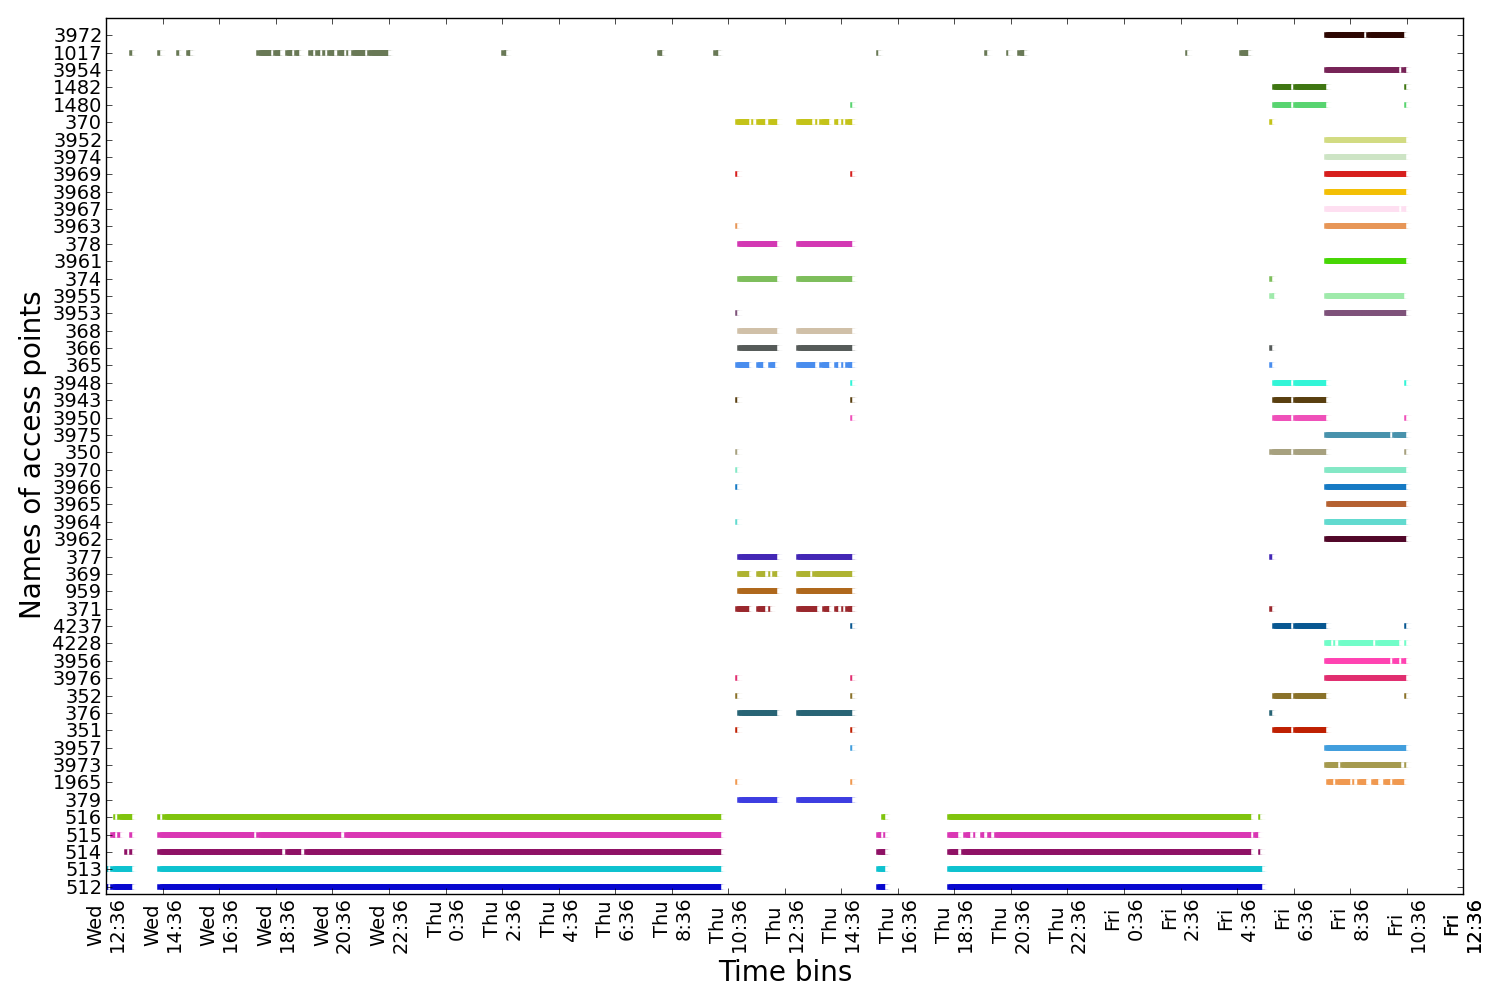
\includegraphics[width=\textwidth]{figures/kmeans/user_3_sorted_2days_no_rssi_plot.png}
\caption{The most common 50 APs for userY during the given 2 days (presence
visualization calculated for 5 minutes time bins)}
\label{user_3_days1_2_APs_presence}
\end{figure}

\begin{figure}[!h]
\centering
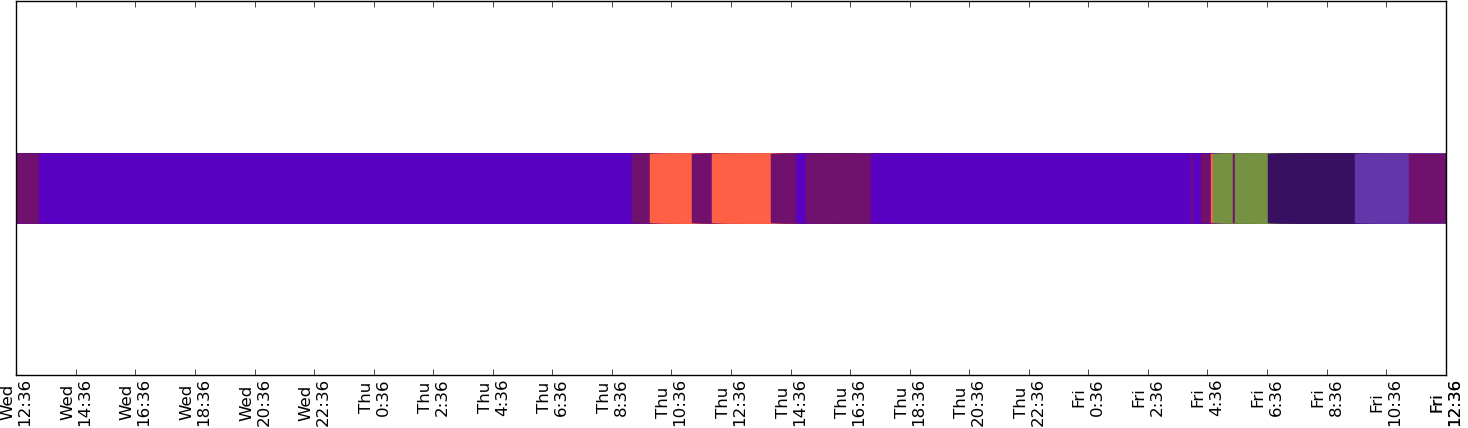
\includegraphics[width=0.95\textwidth]{figures/kmeans/kmeans_locations_(6)_2days_plot.png}
\caption{Locations estimated with k-means for userY for 2 days}
\label{user_3_days1_2_kmeans}
\end{figure}

An additional example of locations estimated using k-means can be seen in
Appendix~\ref{appendix_kmeans}.

\subsection{Hidden Markov Models}
\label{hmm_section}

``Hidden Markov Models (HMMs) are a formal foundation for making probabilistic
models of linear sequence 'labeling' problems. They provide a conceptual
toolkit for building complex models just by drawing an intuitive picture. They
are at the heart of a diverse range of programs, including genefinding, profile
searches, multiple sequence alignment and regulatory site identification. HMMs
are the Legos of computational sequence analysis.''\cite{JOUR} 

HMMs are, in principle, Markov Models (MMs) \cite{opac-b1082850} for which the
modeled systems are considered to be processes with hidden states. If the the
MMs the states are visible to possible observers, the difference for the HMMs is
that the states are not visible, yet the results which can be observed do depend
on the hidden states \cite{18626}.

There area few elements that characterize the HMMs according to \cite{18626}.
They are as follows:
\begin{itemize}
  \item N which represents the number of hidden states in the model. In general,
  these states can be interconnected in a way so that from some states others
  can be reached
  \item M which represents the number of different observation symbols which
  care generated by the hidden states
  \item A which represents the state transition probability distribution. A is a
  matrix for which each element a$_{i,j}$ represents the probability of moving
  from the state i to the state j in the system represented by the HMM
  \item $B = {b_{j}(k)}$ which represents the observation system probability
  distribution in state j. This basically means that each element in B shows the
  probability of seeing a particular element of M in a given state j
  \item $\pi$ which represents the initial state distribution, meaning what is
  the probability of the system to start producing output from any of the states in
  N
\end{itemize}

The three problems also mentioned in \cite{18626} that the HMMs can be used for
to solve are as follows:
\begin{itemize}
  \item Given an observation sequence, how can the probability of the
  observation sequence be computed efficiently considering the given model
  \item Given the observation sequence how can a state sequence be chosen so
  that it explains in the most appropriate manner the existing observations
  \item How can the parameters of the model be adjusted in order to maximize the
  probability of a given observation sequence
\end{itemize}

The second of the three problems above addresses the uncovering of the hidden
states of a given model. Which is exactly what we are trying to identify when
attempting to extract what are the locations an user has been at based on
observing the APs that have been scanned throughout a given time frame for the
given user. In our case, N represents the number of unknown locations a user has
been at, M is the set of observable fingerprints which we can calculate based
on the presence of various APs in $5$ minutes time bins, and A, B and $\pi$ are
the various probability distributions that can be associated with the way in
which the user travels from location to location.

The idea of using HMMs in order to track localization is not new. It has been
explored in papers like \cite{el2013indoor}, \cite{inatomi2013hidden} or
\cite{morelli2007hidden} which sustain the potential of using an algorithm based
on this method of studying the travel behaviour of people.

Scikit-learn \cite{SL} offers an implementation for HMMs that ensures the
training for the models and the inferring of the hidden states and we have been
using the tools they provide for working with our data.

As with the k-means method (Section~\ref{k-means}), the problem we have been
facing was that we could not approximate from the beginning the number of hidden
states (which stand for locations in our case) that we are expecting the model
to find based on the input observations. However, by using the k-fold cross
validation (Section~\ref{cross_valid}) we can, once again (similar to the way in
which we have solved the problem for k-means), test the estimation being
computed based on different numbers of possible locations.

The steps in extracting the locations with the help of the HMM based algorithm
that has been combined with a 10-fold cross validation are as follow:
\begin{itemize}
  \item We select the time frame (number of days) for which we want to extract
  the locations
  \item We retrieve the data and extract the fingerprints
  \item We choose the maximum number of locations we are expecting to find in a
  similar manner we have done for the k-means algorithm, meaning as the minimum
  value between $50$ and the result for the number of days multiplied by $10$
  \item For each possible number of locations in the range of $2$ and our
  previously selected maximum we run the HMM algorithm on the existing
  fingerprints
  \item The estimations are cross validated in order to see which number of
  locations has generated the optimal approximation for the given fingerprints
  \item In case more locations have generated equally good results we select
  as number of expected locations the highest of them
  \item This algorithm is also ran $10$ times leading to $10$ estimations out of
  which the one which appears the most times out of the $10$ results is
  considered the correct one
\end{itemize}

The reason behind running the algorithm $10$ times is the same as the one
present for k-means algorithm. We want to ensure that the random factor which is
involved in the cross validation process has a very little effect on the
correctness of the estimation. At the end of the algorithm we have the hidden
states (in our case, locations) that can be extracted based on the observations
we have based on the presence of the various APs the user is associated to
throughout the given time frame. An example of locations that have been found
for userT throughout $1$ day can be seen in Fig.~\ref{user_6_days1_2_3_hmm}.
They can be easily mapped to the locations we can observe by looking at
Fig.~\ref{user_6_days1_2_3_APs_presence} where we have the presence of the
APs which have been scanned throughout the same amount of time for the same user.
%explain figures
\begin{figure}[!h]
\centering
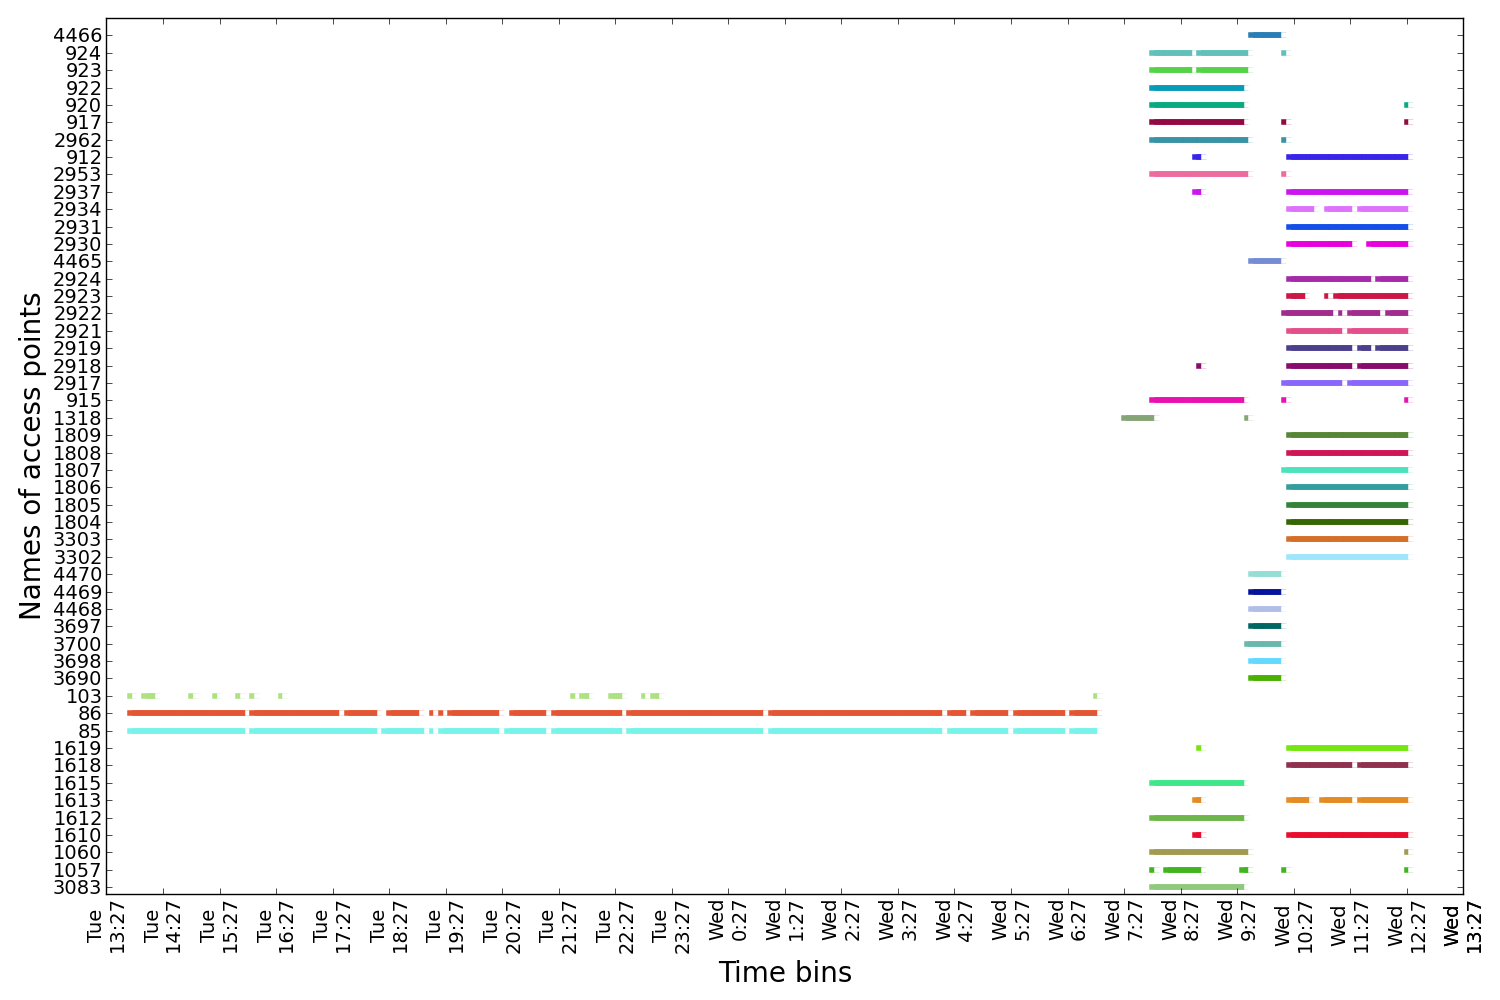
\includegraphics[width=\textwidth]{figures/hmm/user_1_sorted_1days_no_rssi_plot.png}
\caption{The most common 50 APs for userT during the given day (presence
visualization calculated for 5 minutes time bins)}
\label{user_6_days1_2_3_APs_presence}
\end{figure}

\begin{figure}[!h]
\centering
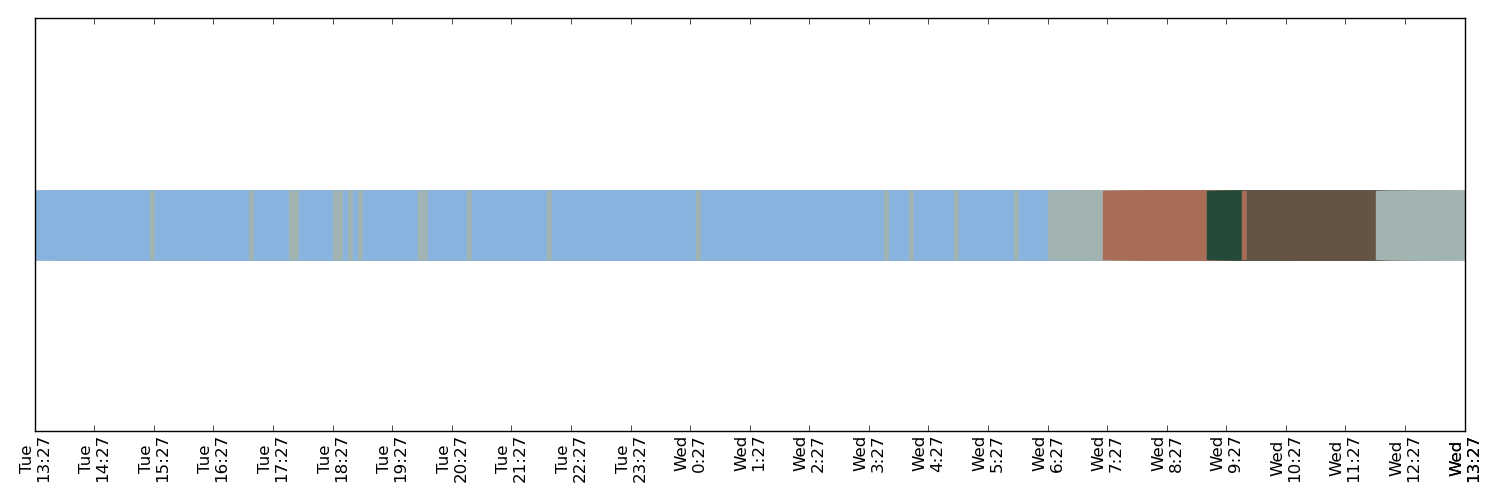
\includegraphics[width=0.95\textwidth]{figures/hmm/user_1_hmm_locations_(5)_1days_plot.png}
\caption{Locations estimated with HMM for userT for 1 day}
\label{user_6_days1_2_3_hmm}
\end{figure}

An additional example of locations estimated using the HMM based algorithm can
be seen in Appendix~\ref{appendix_hmm}.

%\begin{enumerate}
%  \item identifying locations
%	\begin{itemize}
%		\item Hidden Markov Models (5) 
%		\item K-means(2)
%	\end{itemize}
%  \item matching locations locations (0.5)
%	\begin{itemize}
%		\item Percentage similarity (0.5)
%		\item Keeping track of previous locations (0.5)
%		\item Creating fingerprints (1.5)
%	\end{itemize}
%  \item  
%\end{enumerate}                                  %Chapter 2
\chapter{Location matching}
\label{ch_matching}

The HMM method as well as the $k$-means method offer us with the possibility of
extracting locations over a given number of days. However, both the algorithms
perform better when the given time frame is shorter. This finding has come up
while carefully observing the results for different number of days for which the
algorithms have been executed.

The reason behind this behaviour seems to be the limitation of the $10$-fold
cross validation which has been used in order to evaluate the fitness of the
results. The method implies that the data from the time frame taken into
consideration is divided into $10$ equal subsequences which are afterwards used
in turns as training data and as testing data. However, when the data size grows,
the randomly divided subsequences also grow. When we are dealing with
subsequences which have a considerable size, it can happen that some of the
subsequences can contain all of the fingerprints which can be attributed to a
certain location and as such, that location cannot be estimated based on the
other subsequences which have no knowledge of it. This leads to a decay in the
efficiency of estimating the number of locations that we can expect the user
to have been at throughout the evaluated time. The current chapter explores some
possibilities that can help solve this problem.

\section{Methods for solving the ``matching of locations'' problem}

A solution for the previously mentioned problem can be to scale the $k$ factor
of the $k$-fold validation in order to use a factor larger than $10$ when
dealing with bigger amount of data, however this leads to a very long processing
time which can be avoided by using another solution. The second solution is to
extract locations for each day and concatenate the results for all the days
afterwards. This however leads to a new situation. We need to find a way in
which to identify that a location $L_{x}$ from day X might be the same as a
location $L_{y}$ from day Y. This problem is referred to in the present paper
as the ``matching of locations'' problem.

We have taken into consideration three possible ways in which we can solve this
new problem. In order to evaluate the proposed solutions we have evaluated the
results using a graphical approach. We have employed the solutions for a
selection of users for whom we have used the HMM algorithm to identify
locations through a large number of days. Using each proposed solution we have
matched the locations throughout the days and we have observed the accuracy of
the matching that was done.

\subsection{Dictionary of locations based on APs}
\label{dictionary_aps}
The algorithm which can be used for matching up locations over time based on a
\textit{dictionary based on APs} is as follows:
\begin{itemize}
  \item For each location we reunite the time bins that have been associated
  with it. We identify the APs present in either of the time bins and we consider
  all these APs to be associated to the given location
  \item Before adding a new entry in the dictionary~\footnote{Adding an entry
  in such a dictionary is equivalent with defining a new location based on the
  APs of which presence the new location is characterized by.}, we can first
  check the dictionary for previously defined locations that seem to resemble
  the new one based on the APs that define them
  \item If we do not find a similar location we can just add a new entry for the
  new location in the dictionary
  \item If we find locations which resemble the new one in a proportion bigger
  than a given threshold (they have a sufficient number of APs that coincide
  with the ones associated to the new location), we can choose the one which
  resembles the most and consider that the new location and this specific
  location are the same
  \item In the above case, the entry for the location in the dictionary is
  updated to contain the reunion of the APs which define the previous definition
  of the location and the newly found location that matches it
\end{itemize}

This method seems to be a simple solution, however, at a close exploration of
possible situations which can appear within our data we identified a case in
which this solution fails. Let us explore the situation in
Fig.~\ref{overlap_of_aps}. 

\begin{figure}[!h]
\centering
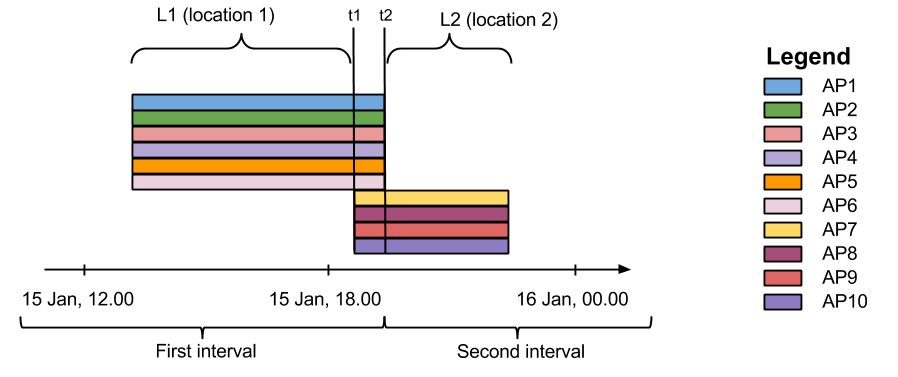
\includegraphics[width=0.95\textwidth]{figures/matching/overlap_of_aps.png}
\caption{Example of APs overlapping}
\label{overlap_of_aps}
\end{figure}

In this case the user would spend most of his or her time for the exemplified
duration at location L1 or at location L2. However, these locations can be, for
example, two rooms which are close enough so as to have a signal overlap between
them (e.g. between t1 and t2). If the user is to stop for enough time, but not
very long (e.g. $5$ minutes which is the duration of exactly one time bin) in an
intermediate location where the signals from the APs in the two rooms overlap,
then the extraction algorithm would identify the location as one of either L1 or
L2. When using the matching algorithm, the dictionary will contain an entry for
L1 which has all the APs from $1$ to $10$ as all of them have been identified
throughout the time in which the user seems to be situated at location L1.
Because of this, when the algorithm tries to see if location L2 can be matched
with another previous location, since the APs attributed to L2 are AP7-AP10,
then all of them can also be found in the entry existing for location L1 and as
such the algorithm considers that locations L1 and L2 are the same.

Situations like this one make the use of this particular algorithm to be
inefficient.

\subsection{Dictionary of locations based on fingerprints}
\label{dictionary_fingerprints}
The algorithm which can be used for matching up locations over time based on a
\textit{dictionary based on fingerprints} is as follows:
\begin{itemize}
  \item For each location identified with our location extraction algorithm and
  for each time bin in which the location appears we can see which is the
  fingerprint~\footnote{A fingerprint is calculated for each time bin. It is a
  list with $N$ elements, where $N$ is the number of APs which are associated
  with the given user. Element at position $i$ in the list is attributed to $AP_{i}$.
  Each element can be either $0$ or $1$ marking the absence or presence in the
  given time bin of the AP which corresponds to the element.} for the given time bin 
  \item An entry in the dictionary can contain the fingerprints which are
  extracted from the time bins that are associated to the location for which
  the entry is created
  \item Before adding a new entry in the dictionary, we can first
  check the dictionary to see if any previously defined location might fit the
  characteristics of the new location we are trying to add~\footnote{Meaning
  that a high number of fingerprints are common to both locations}
  \item If a similar location is not found, we can proceed with adding a new
  entry in the dictionary for the new location
  \item If we find locations which resemble the new one in a proportion bigger
  than a given threshold (which happens when they have sufficient fingerprints
  in common), we can chose the one which resembles the most and consider that
  they are the same
  \item In the above case, the entry for the location in the dictionary
  is updated to contain the reunion of the fingerprints which are attributed
  to the previously defined locations which are now matched into one
\end{itemize}

This solution eliminates the problem that was found in
Section~\ref{dictionary_aps} since, in this case the entries for location L1 and
L2 would be different as it can be seen in
Tab.~\ref{tab:table_fingerprints}~\footnote{We make the assumption that the
algorithm for extracting locations associates the period between t1 and t0 to
location L1.}.

\begin{table}[!h]
\begin{tabular}{|c|c|c|c|}
\hline
\multicolumn{1}{|l|}{}       & \multicolumn{2}{c|}{\textbf{Location 1 (L1)}}   & \textbf{Location 2 (L2)} \\ \hline
\textbf{Access points (APs)} & \textbf{Fingerprint 1} & \textbf{Fingerprint 2} & \textbf{Fingerprint 1}   \\ \hline
AP1                          & 1                      & 1                      & 0                        \\
AP2                          & 1                      & 1                      & 0                        \\
AP3                          & 1                      & 1                      & 0                        \\
AP4                          & 1                      & 1                      & 0                        \\
AP5                          & 1                      & 1                      & 0                        \\
AP6                          & 1                      & 1                      & 0                        \\
AP7                          & 0                      & 1                      & 1                        \\
AP8                          & 0                      & 1                      & 1                        \\
AP9                          & 0                      & 1                      & 1                        \\
AP10                         & 0                      & 1                      & 1                        \\ \hline
\end{tabular}
\caption{This table shows the fingerprints for locations L1 and L2 in
Fig.~\ref{overlap_of_aps}}
\label{tab:table_fingerprints}
\end{table}

There is, however, another situation which we were able to identify and which
creates difficulties for the good functionality of the present algorithm. The
mentioned case can be seen in Fig.~\ref{diff_fp_same_loc}

\begin{figure}[!h]
\centering
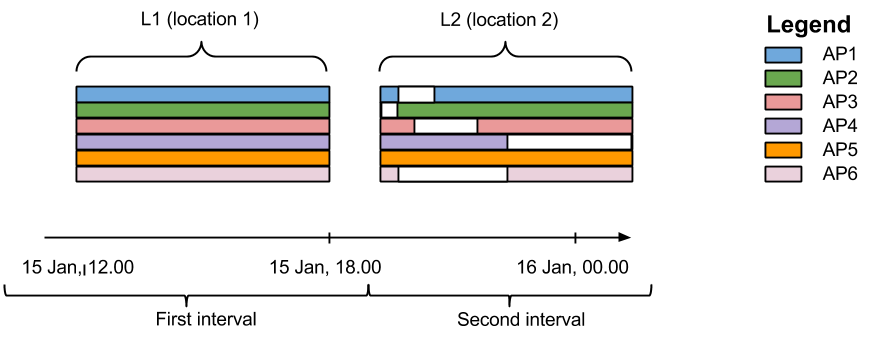
\includegraphics[width=0.95\textwidth]{figures/matching/different_fp_same_loc.png}
\caption{Example of locations which can be matched yet do not have any identical
fingerprints overlapping}
\label{diff_fp_same_loc}
\end{figure}

The fingerprints of locations L1 and L2 in this new case can be seen in
Tab.~\ref{tab:table_fingerprints_same_loc}. As we can see there are no common
fingerprints identified for the two locations because in the case of location L2
the signal from the APs that identify with it is not constant because of
possible interferences. In this case the algorithm will fail to identify the two
location as being the same one and, as such, the present algorithm can present
difficulties when solve the matching problem.

\begin{table}[!h]
\begin{tabular}{|c|c|c|c|c|c|c|c|}
\hline
             & \textbf{Location 1 (L1)}     & \multicolumn{6}{c|}{\textbf{Location 2 (L2)}}                                           \\ \hline
\textbf{APs} & \textbf{Fingerprint 1 (FP1)} & \textbf{FP1} & \textbf{FP2} & \textbf{FP3} & \textbf{FP4} & \textbf{FP5} & \textbf{FP6} \\ \hline
AP1          & 1                            & 1            & 0            & 0            & 1            & 1            & 1            \\
AP2          & 1                            & 0            & 1            & 1            & 1            & 1            & 1            \\
AP3          & 1                            & 1            & 1            & 0            & 1            & 1            & 0            \\
AP4          & 1                            & 1            & 1            & 1            & 1            & 0            & 1            \\
AP5          & 1                            & 1            & 1            & 1            & 1            & 1            & 1            \\
AP6          & 1                            & 1            & 0            & 0            & 0            & 1            & 0            \\ \hline
\end{tabular}
\caption{This table shows the fingerprints for locations L1 and L2 in
Fig.~\ref{diff_fp_same_loc}}
\label{tab:table_fingerprints_same_loc}
\end{table}

\subsection{Dictionary of location signatures}
\label{dictionary_signatures}
We define the signature of a location as follows:
\begin{itemize}
  \item It is an entity which is calculated for a location taking into
  consideration a given period of time (for example $1$ day) for which we have
  used an algorithm for extracting the locations
  \item It is an entity which identifies a location independently of the moment
  of time inside the time frame for which it is calculated (as opposed to the
  fingerprints that have been mentioned in 
  Section~\ref{dictionary_fingerprints} and which are extracted for each time bin)
  \item It is a list of $N$ elements (where $N$ is the number of APs which the
  user is associated with)
  \item Each element has the value $1$ or $0$
  \item If the element at position $i$ in the list (where $i \in \{1..N\}$) is
  $1$ it means that the associated AP ($AP_{i}$) has been found mostly with the
  value $1$ in the fingerprints associated to the existing time bins (as
  presented in Section~\ref{dictionary_fingerprints}) and if it is $0$
  it means the opposite~\footnote{This means that if the signature of the
  location we are interested in has the element attributed to a given AP set to
  $1$ then the AP has appeared in more time bins than the ones it was missing
  from during the given time frame. If it is $0$, than the AP has been missing
  from more time bins than the ones that it was present in and that are
  associated to the give location.}
\end{itemize}

The way in which these signatures are create eliminates the problems that can
appear in case interferences appear and disturb the presence of the signal from
various APs for a limited amount of time. The location matching algorithm, in
this case, can be as follows:

\begin{itemize}
  \item We calculate the location signature for each location identified with
  our location extraction algorithm throughout a given number of days
  \item An entry (which is associated to a location) in the dictionary contains
  the location signature
  \item Before adding a new entry in the dictionary, we can first
  check the dictionary to see if any of the previous locations have a signature
  that is similar above a selected threshold to the one of the new location we
  are trying to add
  \item If a similar location is not found, we can proceed with adding a new
  entry in the dictionary for the new location
  \item If we find a location which resembles the new one in a proportion bigger
  than a given threshold then we can consider that the two are the same
  location
\end{itemize}

The similarity between two signatures is calculated by taking into consideration
the APs that are set to $1$ in either of the two signatures and the APs which
are set to $0$ but that are present in both signatures~\footnote{The difference
in APs in signatures is given by the fact that, when looking at data from
different days, the APs which are scanned during these days might not always be
the same. We are not keeping all the APs associated at any moment with a user
because this leads to an unnecessary increase in the execution time.}. The
similarity value si calculated as the number of APs that have the same value
associated to them in both the signatures (either $0$ or $1$) and this number is
then divided to the number of APs in the reunion.

The similarity result obtained for two signatures is compared to a given
threshold in order to determine if the two signatures are referring to the
same geographical location. We have experimented with threshold values between
$65\%$ - $98\%$ and the results show that threshold values inside the
interval $75\%$ - $80\%$ return the most accurate results for matching
locations.

By analysing data for different users we found a case in which this method did
not identify correctly that two locations where in fact the same one. The
situation can be seen in Fig.~\ref{same_location_less_than_threshold}.

\begin{figure}[!h]
\centering
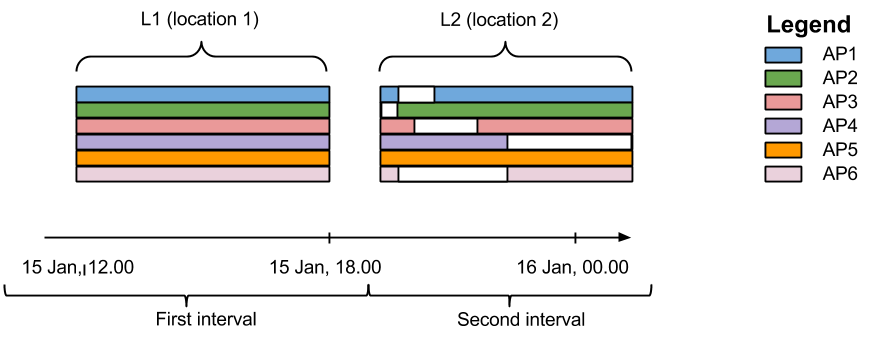
\includegraphics[width=0.95\textwidth]{figures/matching/different_fp_same_loc.png}
\caption{Example of locations which need to be matched despite their similarity
being below the threshold}
\label{same_location_less_than_threshold}
\end{figure}

As we can see, location L1 has $10$ APs while location L2 has only $5$. Since
the APs in location L2 are also present in location L1 it is safe to assume that
the remaining APs are not present in L2 due to technical problems or
interferences. However, when calculating the signatures of the two locations and
comparing them, by using a threshold value of $80\%$ for considering them the
same, we would only obtain that they are similar in a $50\%$ proportion. In
order to avoid this kind of situations, we have added to our algorithm another
condition which goes as follows: if all the APs which have the value $1$ in the
signature of a location appear in the signature of an already found previous
location, than the two can be considered the same location even if the
similarity value is not above the given threshold. This small improvement
ensures that the algorithm performs well even despite cases as this one.

This third possible solution performs well for the test we have conducted over
or data and as such it has been chosen for solving the matching problem for
locations over different days.
                                  %Chapter 2
\chapter{Entropy and predictability}

The potential of using a real scientific approach in order to be able to predict
where people will travel in the near or less near future can have an outstanding
impact on the way in which the engineers design and construct infrastructures
for cities, it can also impact the way in which we understand the transportation
system and, not to mention, it could give us a new insight into how we can
approach the solving of epidemics spreading \cite{Lu13} \cite{Brockmann08}.

Data from SensibleDTU \cite{Stopczynski14m} allows us to explore for research
purpose exactly how and why people move from a certain location to another. It
gives us the opportunity to look more careful into our mobility patterns in
order to try to understand how we can make use of these patterns to improve our
world.

%TODO -add no of users
In order to explore the entropy and predictability of human mobility, we have
conducted tests based on the data retrieved from a selection of users from the
SensibleDTU database. We have selected $65$ users from our original pool of
$131$ users in order to observe their movements throughout a period of $30$ days. The
reason behind discarding the remaining users was that their data was found to be
missing important fields or they did not keep their mobile phones charged and
open for the most part of the $30$ days and thus their result could have
jeopardize the study results.

\section{Entropy}

``Entropy is probably the most fundamental quantity capturing the degree of
predictability characterizing a time series'' \cite{Barabasi10}. Multiple
studies (\cite{Sinatra14},\cite{Lu13}, \cite{marin2012exploring},
\cite{Barabasi10}) that aim at understanding the predictability of the human
travel trajectory take into consideration different entropy measures which have
different meaning and different levels of importance in correctly estimating the
probability of choosing a location or another. The measures that are mentioned
are the random entropy, the temporal uncorrelated entropy, the conditional
entropy and the real entropy.

\subsection{The random entropy}
\label{r_e}

The formula for the random entropy of a random user i is given by

\begin{equation}
S_{i}^{rand} = log_{2}N_{i}
\end{equation}

Where $N_{i}$ represents the number of unique locations that
have been associated to the given user throughout the time frame that we are
taking into consideration. This measurement can be used to reflect the
predictability of the travel patterns of the given user in case we consider that
each of the locations can be visited with the exact same probability.

We have calculated the random entropy by taking into consideration the locations
visited by our selected users throughout a period of $30$ days.
Fig.~\ref{dis_r_e} shows the density distribution of the results which have been
rounded after the second decimal. As we can see, most of the users have a random
entropy of around $3.65$ and the average random entropy is $3.87$. This means
that, in average, is a user would choose randomly his or her next location, than
they can be found in any of $2^{S^{rand}} = 2^{3.87}$ locations (which is
approximately $14.62$).

\begin{figure}[!h]
\centering
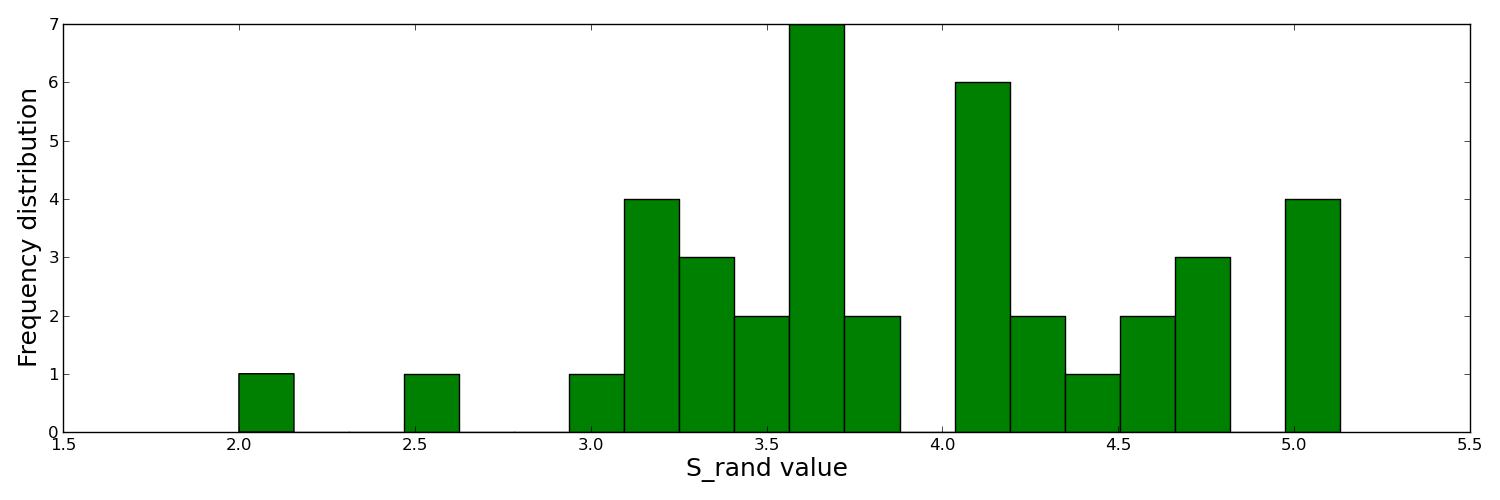
\includegraphics[width=\textwidth]{figures/entro_pred/rand_entro_distrib.png}
\caption{Density distribution for $S^{rand}$}
\label{dis_r_e}
\end{figure}

\subsection{The temporal uncorrelated entropy}
\label{tu_e}

The formula for the temporal uncorrelated entropy of a random user i is given by

\begin{equation}
S_{i}^{unc} = -\sum\limits_{j=1}^{N_{i}}p_{i}(j)log_{2}p_{i}(j)
\end{equation}

Where $N_{i}$ represents the number of unique locations that have been
associated to the given user throughout the time frame that we are taking into
consideration and $p_{i}(j)$ represents the historical probability of the given
user to visit location j. The present measurement incorporates the knowledge
about what locations occur more often in the user's traveling patterns.

We have calculated the temporal uncorrelated entropy by taking into
consideration the locations visited by our selected users throughout a period of
$30$ days. Fig.~\ref{dis_tu_e} shows the density distribution of the results
which have been rounded after the second decimal. The average temporal
uncorrelated entropy is $1.3$. This means that, in average, if we are to base
our supposition on the number of times each location has been visited in the
past by a given user, then the user's next location can be found in any of
$2^{S^{unc}} = 2^{1.3}$ locations (which is approximately $2.46$).

\begin{figure}[!h]
\centering
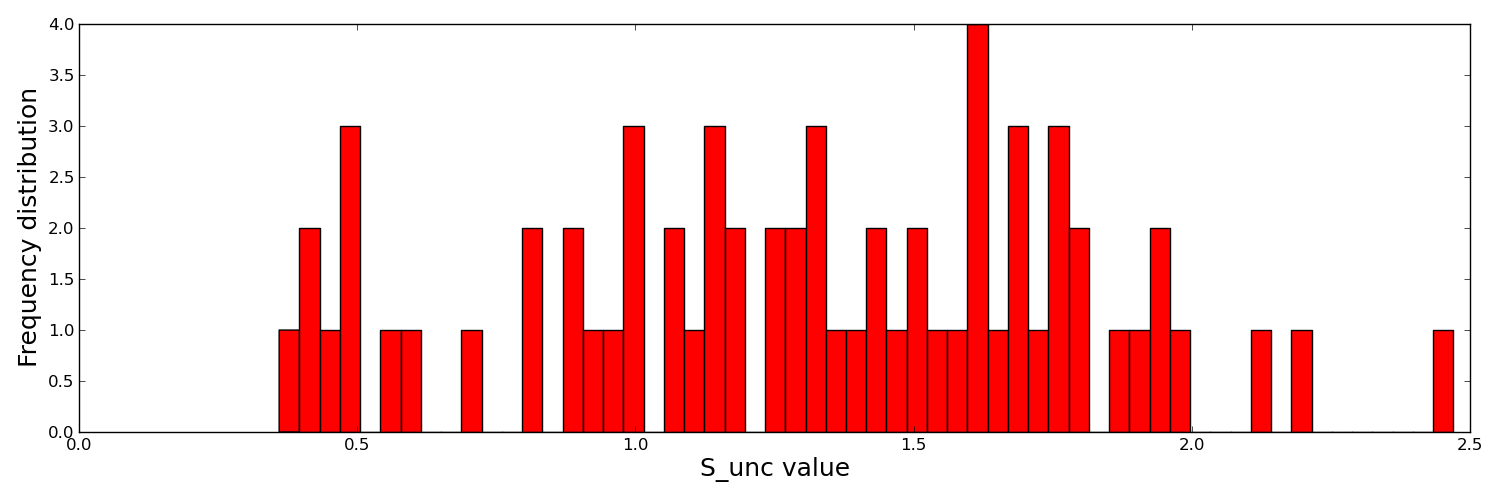
\includegraphics[width=\textwidth]{figures/entro_pred/tu_entro_distrib.png}
\caption{Density distribution for $S^{unc}$}
\label{dis_tu_e}
\end{figure}

\subsection{The conditional entropy}
\label{con_e}
The conditional entropy $S_{i}^{cond}$ for a given user $i$ is calculated based
on the formula given in the paper \cite{Sinatra14}

\begin{equation}
S_{i}^{cond} = - \sum\limits_{x_{t}\in X_{i}} \sum\limits_{x_{t-1}\in X_{i}}
p_{i}(x_{t-1},x_{t})log_{2}p_{i}(x_{t}|x_{t-1})
\end{equation}

In this formula, $x_{t}$ and $x_{t-1}$ are possible locations,
$p_{i}(x_{t-1},x_{t})$ is the probability of apparition of the subsequent
locations $x_{t-1}$ and $x_{t}$ and $p_{i}(x_{t}|x_{t-1}) = p_{i}(x_{t-1},x_{t})
/ p(x_{t-1})$ represent the probability of the user being at location $x_{t}$ at
time $t$, considering that the previous location was $x_{t-1}$. The conditional
entropy is equal to the temporal uncorrelated entropy in case we do not make any
time correlations. Also it can be proved that $S^{cond} \leq S^{unc} \leq
S^{rand}$ \cite{Cover:2006:EIT:1146355}.

In \cite{Sinatra14} the authors introduce an extension for the conditional
entropy in order to explore how the amount of previous knowledge affects the
value of the conditional entropy. The new formula is 

\begin{equation}
S_{i}^{cond,k} = - \sum\limits_{x_{t}\in X_{i}} .. \sum\limits_{x_{t-k}\in
X_{i}} p_{i}(x_{t-k},..,x_{t})log_{2}p_{i}(x_{t}|x_{t-k},..,x_{t-1})
\end{equation}

In this case, k represents the number of previous steps we know. With the
present formula it can be observed that $S_{i}^{cond,0}$ is the same with
$S_{i}^{unc}$ and that $S_{i}^{cond,1}$ is the same as $S_{i}^{cond}$.

In Fig.~\ref{conditional_e} we have the representation for the conditional
entropy calculated considering that we have knowledge of a previous time window
of $1 - 30$ time bins. It can be seen that the more information we have from the
past, the value of the conditional entropy decreases.

\begin{figure}[!h]
\centering
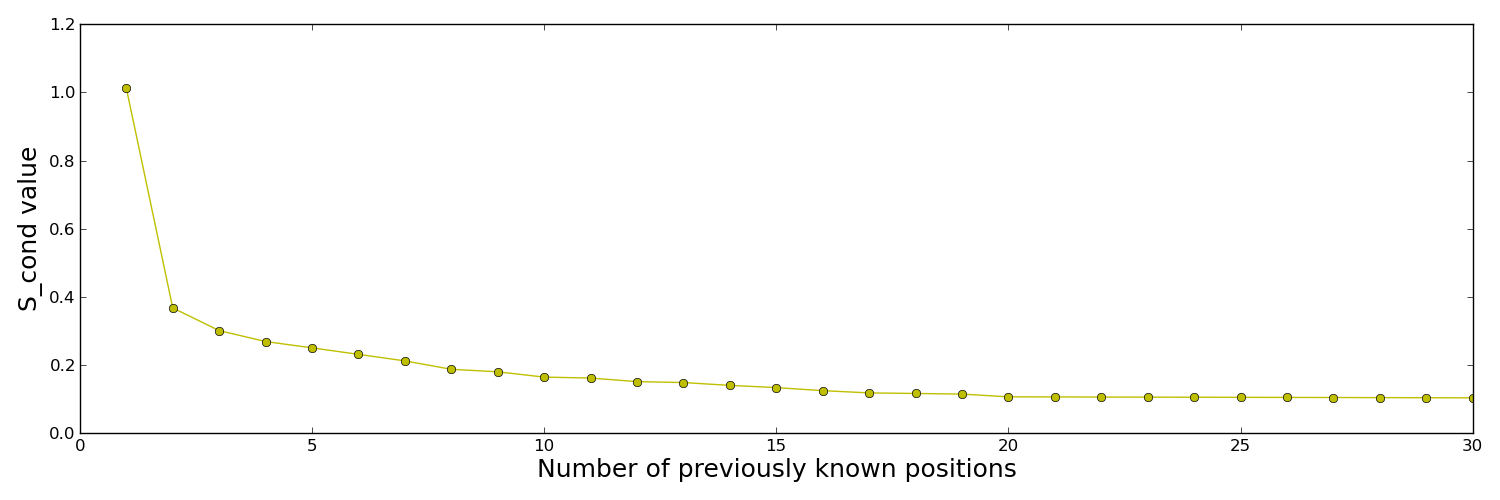
\includegraphics[width=\textwidth]{figures/entro_pred/constr.png}
\caption{$S^{cond,k}$ for a given user, where $ k \in \{1,..30\}$}
\label{conditional_e}
\end{figure}

\subsection{The real entropy}
The real entropy of a user needs to be calculated by taking into consideration
the different locations that the user has been to, the frequency with which he
or she visits these locations, the time spent at the locations and the order in
which the locations seem to follow through time. The relation between the actual
entropy and the random and time uncorrelated entropies is $S \leq S^{unc}
\leq S^{rand}$. 

If we consider that $X_{i}$ represents the locations of a user at time i,
and $h_{n}$ represents a sequence of n locations, then for a process X =
\{$X_{i}$\} the entropy can be written as
\begin{equation}
\label{eq_7_5}
S \equiv \lim_{n\to\infty} {1 \over n}S(X_{1},X_{2},..,X_{n})
\end{equation} 
\begin{equation}
\label{eq_7_6}
= \lim_{n\to\infty} \sum\limits_{i=1}^{n} S(X_{i}|h_{i-1})
\end{equation}
\begin{equation}
\label{eq_7_7}
= \lim_{n\to\infty} \sum\limits_{i=1}^{n} S(i)
\end{equation}

Equation \ref{eq_7_5} is the definition given to entropy in
\cite{Cover:2006:EIT:1146355}, equation \ref{eq_7_6} reflects the application of
the chain rule in the previous equation and $S(X_{i}|h_{i-1})$ represents the
conditional entropy at step n in equation \ref{eq_7_7} \cite{song2010limits}.

The paper \cite{Barabasi10} present another way in which the entropy for a user
i can be written. If we consider that $T_{i} = {X_{1}, X_{2},\ldots, X_{n}}$
represents the sequence of locations which have been visited by user i and if we
consider that $P(T'_{i})$ represents the probability of finding time ordered
subsequence $T'_{i}$ in the trajectory $T_{i}$, then the entropy of user i can
be written as

\begin{equation}
S_{i} = - \sum\limits_{T'_{i}\subset T_{i}}P(T'_{i})log_{2}[P(T'_{i})]
\end{equation}

We have calculated a measurement of the entropy for our selected users and the
distribution for the results which have been rounded after the second decimal
can be seen in Fig.~\ref{dis_full_e}. The fact that the average value of the
real entropy for the selected user is around $0.17$ means that, in reality we
the uncertainty about where a user will be traveling to next is $2^{0.17} =
1.12$ locations. These findings show that, the users we have been observing do
not randomly choose their future locations, but in fact, their locations are
well established by restrictions such as hours or days at which they need to be
at work, or school as well as other patterns that govern most of the times our
decisions.

\begin{figure}[!h]
\centering
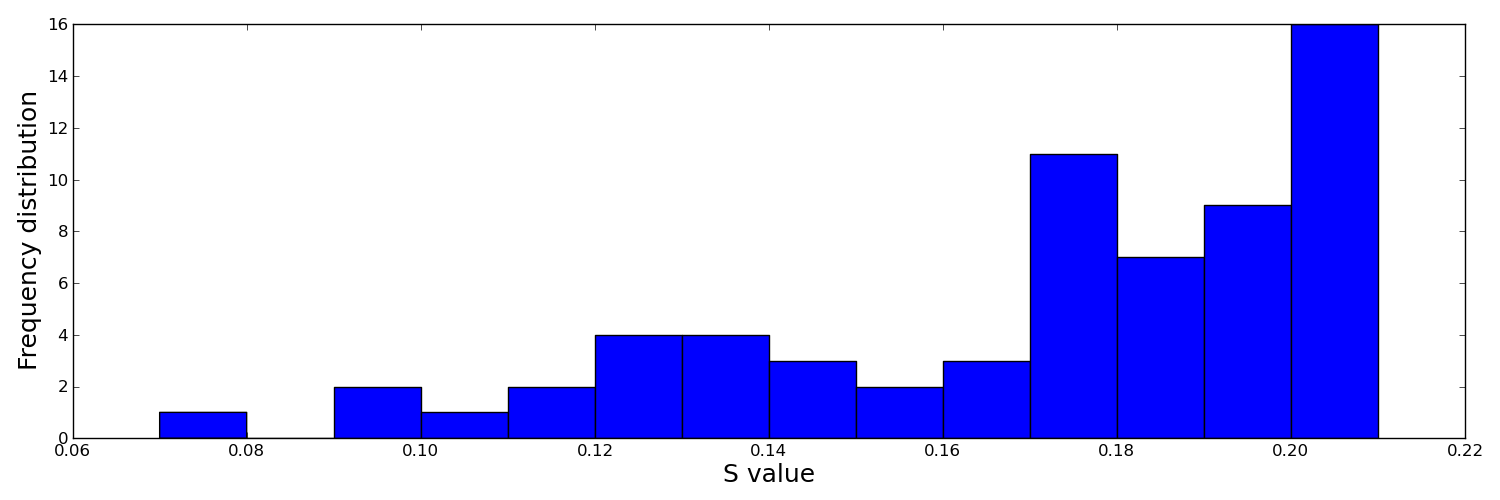
\includegraphics[width=\textwidth]{figures/entro_pred/full_entro_distrib.png}
\caption{Density distribution for $S$}
\label{dis_full_e}
\end{figure}

In Fig.~\ref{dis_overlay} we have an overlay of the distribution for the random,
temporal uncorrelated and real entropies.

\begin{figure}[!h]
\centering
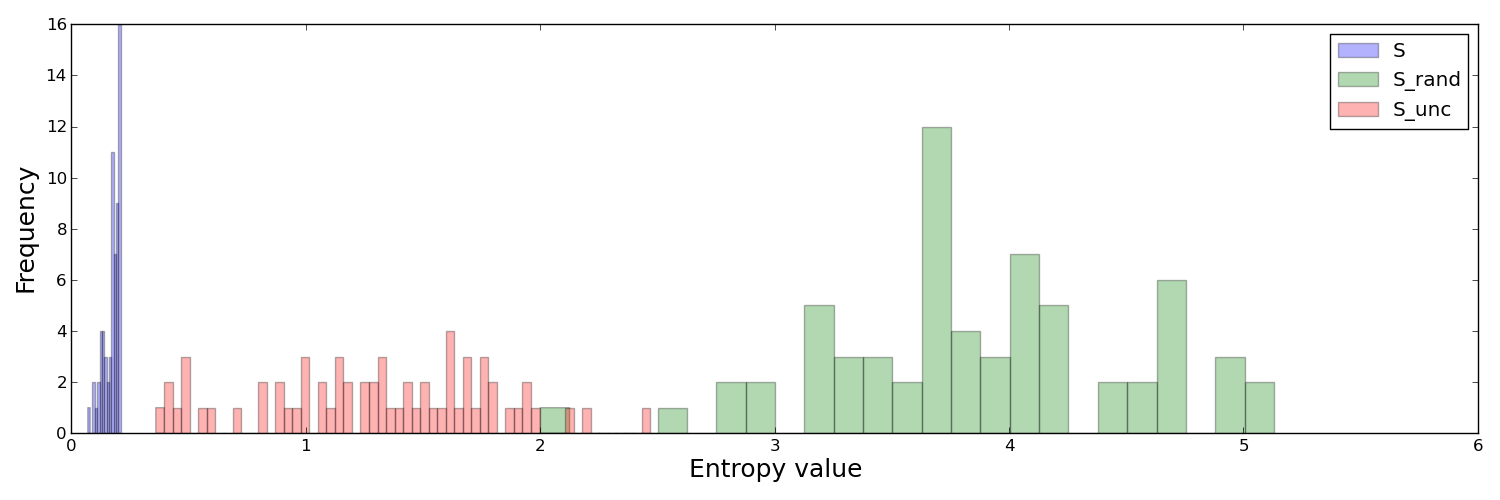
\includegraphics[width=\textwidth]{figures/entro_pred/overlay.png}
\caption{Density distributions for $S$, $S^{rand}$ and $S^{unc}$}
\label{dis_overlay}
\end{figure}

\section{Predictability}

A measure that needs to be taken into consideration when discussing
predictability is the probability ($\Pi$) of a predictive algorithm to correctly
estimate the future locations a user will visit. According to the inequality of
Fano \cite{brabazon2008natural} \cite{1057678}, a user for which the entropy is
S and it has been calculated taking into consideration the fact that the user
spends his or her time in either of N given locations, then his or her
predictability (as it is presented in \cite{Barabasi10} and in \cite{Sinatra14}
as well) is given by

\begin{equation}
\label{ineq_pred}
\Pi \leq \Pi^{max}(S,N)
\end{equation}

The value for $\Pi^{max}$ can be determined from

\begin{equation}
\label{pred}
S = H(\Pi^{max}) + (1 - \Pi^{max})log_{2}(N-1)  
\end{equation}

by knowing that

\begin{equation}
\label{h_func}
H(\Pi^{max}) = - \Pi^{max}log_{2}(\Pi^{max}) - (1-\Pi^{max})log_{2}(1-\Pi^{max})   
\end{equation}  

By combining the two previous formula we obtain the equation

\begin{equation}
\label{equation}
S + \Pi^{max}log_{2}(\Pi^{max}) + (1-\Pi^{max})log_{2}(1-\Pi^{max}) - (1 -
\Pi^{max})log_{2}(N-1) = 0
\end{equation}

One of the aims of our study is to estimate the predictability when it comes to
the trajectory patterns of the selected users from the SensibleDTU database.
After we have calculated their entropy and after knowing the number of locations
each of them has been traveling in between for the duration of $30$ days that we
considered for our experiment, we only needed to calculate the entropy based on
the mathematical formulae at \ref{pred} and \ref{h_func}. However, the equation
at \ref{equation}, which would allow us to calculate the predictability for each
user is a transcendent equation. This means that the equation can be solved
either numerically or graphically.

In order to solve the equation we use a numerical method that helped us
approximate the result. The method we use is the bisection method \cite{faires}.
This method is applicable for solving an equation $f(x) = 0$ over a given
interval $[a,b]$ for which the values $f(a)$ and $f(b)$ have opposing sings. In
our case the f function is represented by the left side in the equation
\ref{equation}. Since the solution of our equation $f(x) = 0$ needs to be a
number between 0 and 1 (the maximum predictability can only have a value in this
interval), than we start the algorithm by verifying if by replacing the maximum
predictability with 0 or 1 we have a solution or if the two values obtained this
way have opposing signs. If they have opposing signs, we consider that $a = 0$
and $b = 1$. In case the function does not have opposing signs, we adjust the
interval until we find either a solution or values for which the signs are
opposing. The algorithm continues as following:
\begin{itemize}
  \item As long as we do not exceed a previously set number of iterations we
  look for the middle of the interval given by the selected a and b numbers
  (let the middle be m)
  \item In case $f(m)$ is 0 or sufficiently close to 0 (we accept an error of
  order $10^{-3}$), than we have found our solution, otherwise if the value of
  $f(m)$ has the same sign as $f(a)$ we move forward considering the interval
  $[m,b]$, if it has the same sign as $f(b)$ we continue by using the interval
  $[a,m]$
  \item We increment the number of iterations we have computed
\end{itemize}

The average predictability value for the selected users and through the given
$30$ days of observations is of approximately $98\%$ which supports the
observations made in previous studies (a considerable number of which have
already been mentioned in the present paper - e.g. \cite{song2010limits},
\cite{Barabasi08} etc) regarding the fact that we seem to have a highly well
established pattern of traveling that rises from our daily habits.

% 6 pages \begin{enumerate} \item Calculating entropy for users \item
% Calculating predictability for users \item Observations end{enumerate}
                                  %Chapter 2
\chapter{Wifi versus GPS locations}
\section{Extracting stop locations from GPS data}
\section{Comparing results with GPS data}
% 5 pags                                  %Chapter 2
\chapter{Future work}
% 1 page
\chapter{Conclusions}

This paper discusses the steps which have been taken in order to study the
inferring of human mobility patterns from Wifi data. The focus of the study has
been divided in between different areas of this subject. We have firstly
analyzed what defines a Wifi determined location. 

We have taken into consideration different approaches that can be used in order
to extract locations. We considered determining locations based on access
points' BSSIDs and RSS. This option has lead to us trying to find a solution for
a better noise elimination. We have experienced with different averages that
aimed to smooth the spikes in the signal strength, however we have come to the
conclusion that for the used data a better approach is to only take into
consideration the BSSIDs of the access point and the knowledge if an access
point is present of not in a given time bin. The information extracted by
analyzing when the access point are visible is named access point presence and
has been used in order to determine stop locations.

The extraction of the locations based on the identity and presence of various
access points throughout different time framse has proved to be a challenging
and complex task. We have tested three different methods: an algorithm based on
the usage of networks, an algorithm based on k-means clustering and an algorithm
based on Hidden Markov Models. The first algorithm did not lead to satisfactory
results in the present study. Between the second two approaches, the algorithm
based on Hidden Markov Models has statistically had better results through our
used data, however further research is needed in order to make a defined
assumption on which of the two algorithms can prove to be better to use in
different circumstances. Also, in order to use either of k-means or Hidden
Markov Models based algorithms we needed to first determine the number of
locations we were expecting the algorithms to identify. This has been achieved
by the use cross validation.

In order to conduct the study over a large amount of data we needed to run the
location identification algorithm on data collected during smaller time frames
(e.g. one day). The resulting locations have been compared to each other. This
was needed in order to determine if a location appeared in the results from a
different iteration. We have also compared the resulting locations extracted
from Wifi data to locations which have been extracted from analogue GPS data.
The results have been satisfactory in the sense that, even though, as expected,
GPS data can offer more detailed results about location changes, the accuracy
of the Wifi results is not badly impaired.

By knowing the different locations and the sequence in which they occurred
throughout time we were able to calculate various entropy values for a selected
pool of users. We have also been able to determine that the users which have
been selected to be part of the present study present a high degree of
predictability as far as human mobility is concerned. This observation supports
previous results which have been made regarding this topic, yet further research
on an even bigger data set and longer period of time might be needed in order to
establish if this particular observation can be considered a fact.

We have concluded the paper by making a summary of the most important
observations that have emerged throughout our work as well as a series of
suggestions about possible future areas of interest for the present topic.

To conclude, we would like to state that the work in the present field is far
from being complete. There are many questions that still require answers and
many opportunities for improvement and we feel that the findings presented in
the current paper, as well as previous works can constitute a solid ground for
further research projects. The topic in itself is of a high interest for the
future as any results can be used to drastically improve the quality of life for
generations to come.

\appendix
\chapter{Appendix}

\section{Variations for signal strength visualization over time}
\label{appendix_signal_strength}

This section contains various visualizations for different users' scanned access
points over time. On the x axis we have the time frame, while on the y axis we
have the signal strength for the identified access points. The legend presents
only the top $10$ predominant access points (which have appeared the most
during scans), however the plot displays all access points. The figures are
Fig.~\ref{user_6_cross_1d}, Fig.\ref{user_6_star_1d},
Fig.~\ref{user_6_cross_line_1d}, Fig.\ref{user_6_o_line_1d}.

\begin{figure}[!h]
\centering
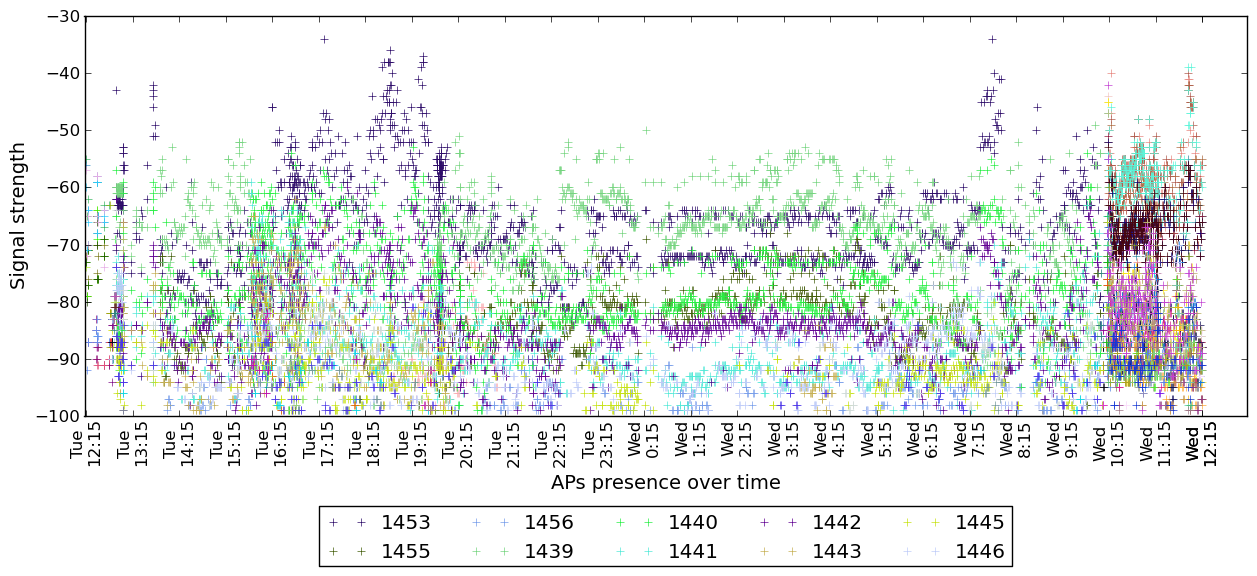
\includegraphics[height =
0.45\textwidth]{figures/cros_user_6_sorted_1days_plot.png}
\caption{Example of the APs registered for userX throughout one day with
``+'' markers}
\label{user_6_cross_1d}
\end{figure}

\begin{figure}[!h]
\centering
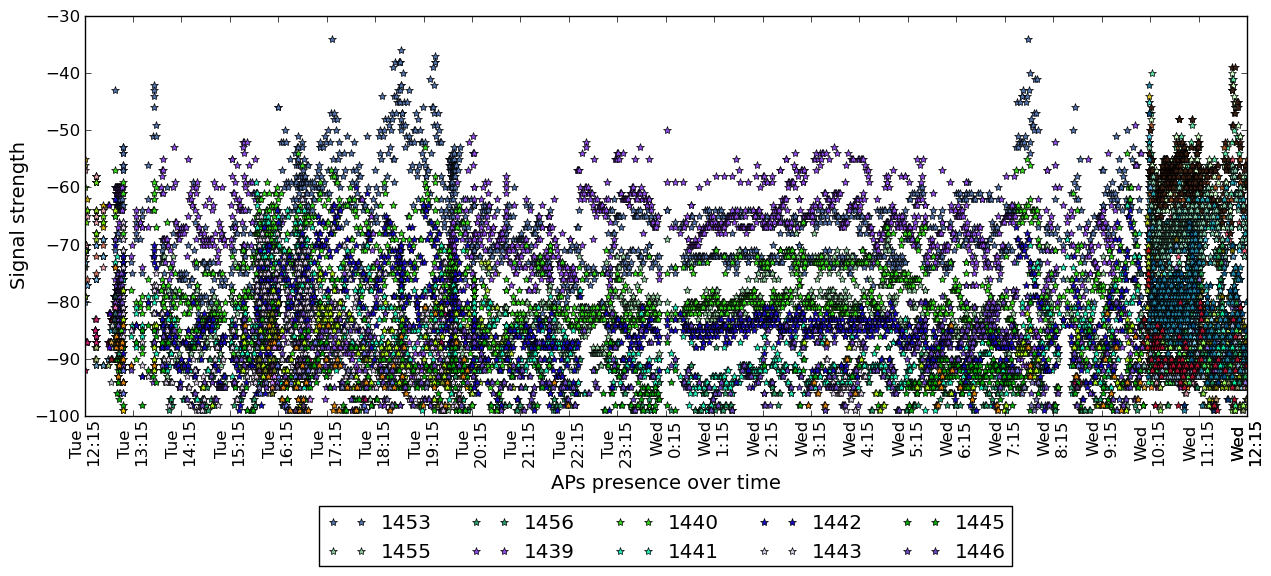
\includegraphics[height =
0.45\textwidth]{figures/star_user_6_sorted_1days_plot.png}
\caption{Example of the APs registered for userX throughout one day with
``*'' markers}
\label{user_6_star_1d}
\end{figure}

\begin{figure}[!h]
\centering
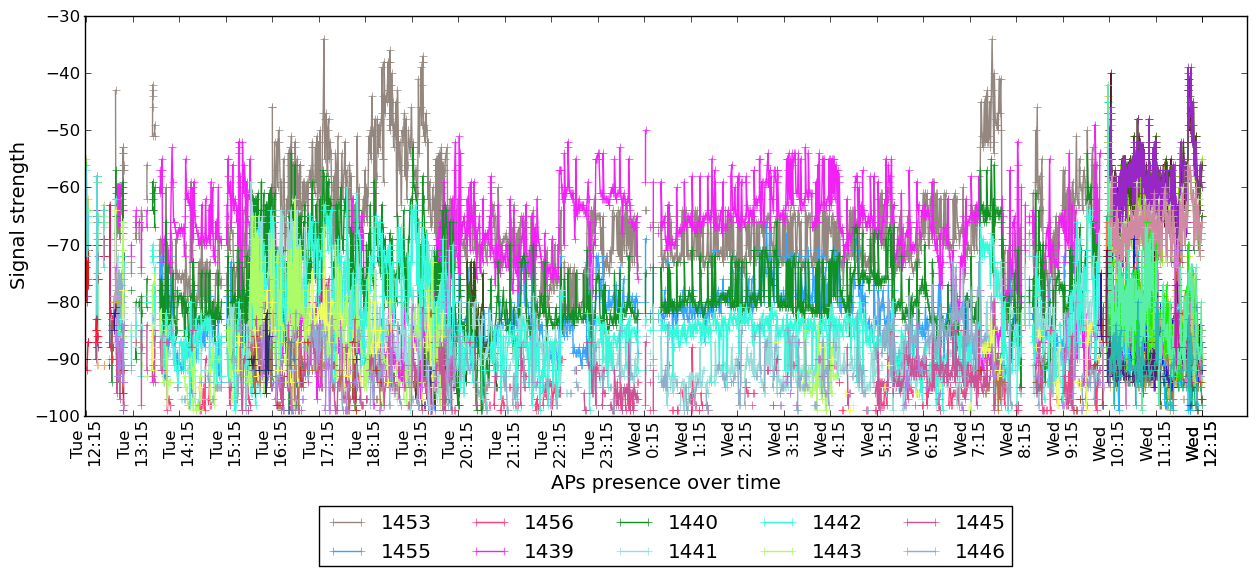
\includegraphics[height =
0.45\textwidth]{figures/cros_line_user_6_sorted_1days_plot.png}
\caption{Example of the APs registered for userX throughout one day with
``+'' and line markers}
\label{user_6_cross_line_1d}
\end{figure}

\begin{figure}[!h]
\centering
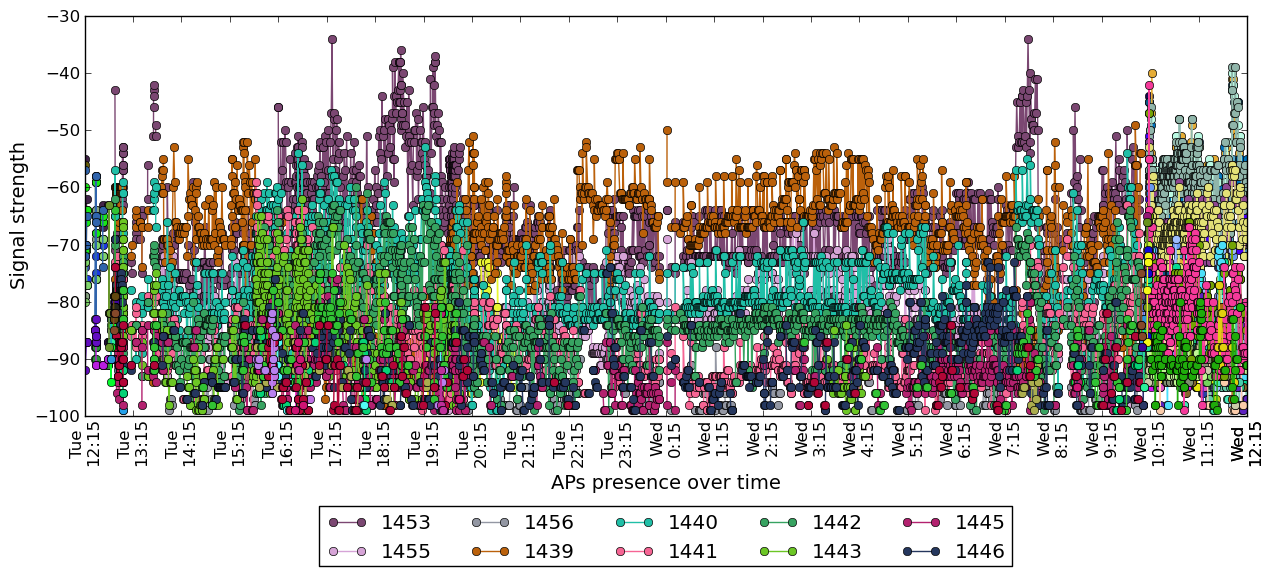
\includegraphics[height =
0.45\textwidth]{figures/o_line_user_6_sorted_1days_plot.png}
\caption{Example of the APs registered for an user throughout one day with
``o'' and line markers}
\label{user_6_o_line_1d}
\end{figure}

\section{Sample density for APs identified for a user}
\label{appendix_sample_density}

This section contains the visualization for the signal strength of different APs
that have been identified as being associated to a user throughout a period of
$1$ day (Fig.~\ref{rssi_6_2nd_day_A}) as well as the sample density
visualizations for the top various APs that were scanned throughout this time
(Fig.~\ref{samples_6_2nd_day_1_A},Fig.~\ref{samples_6_2nd_day_2_A},Fig.~\ref{samples_6_2nd_day_3_A}).

\begin{figure}[!h]
\centering
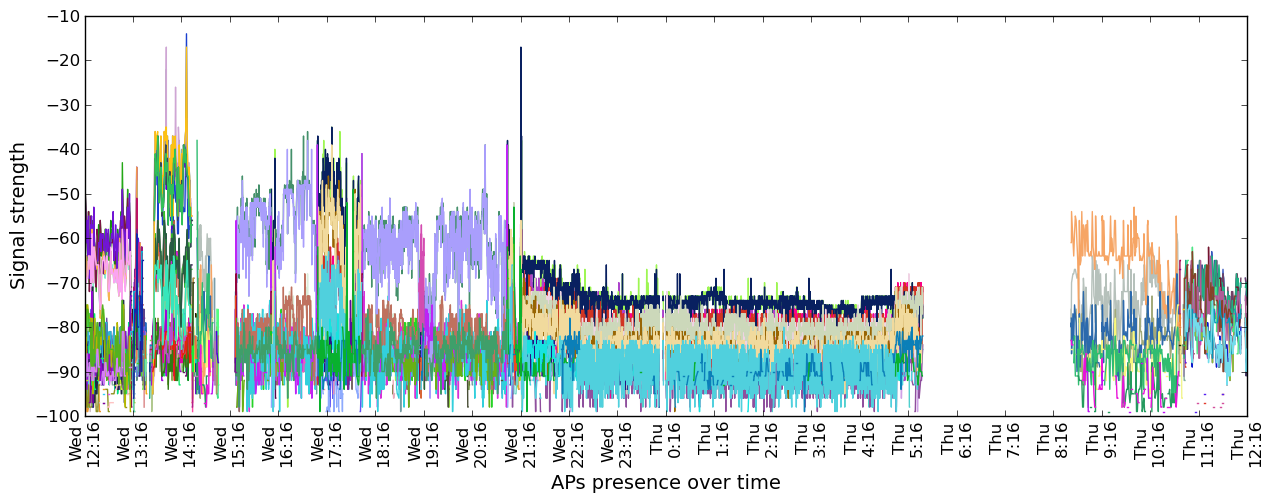
\includegraphics[width =\textwidth]{figures/combinations/user_6_sorted_1days_plot_croped.png}
\caption{Example of the APs registered for userX throughout day 2}
\label{rssi_6_2nd_day_A}
\end{figure}

\begin{figure}[!h]
\centering
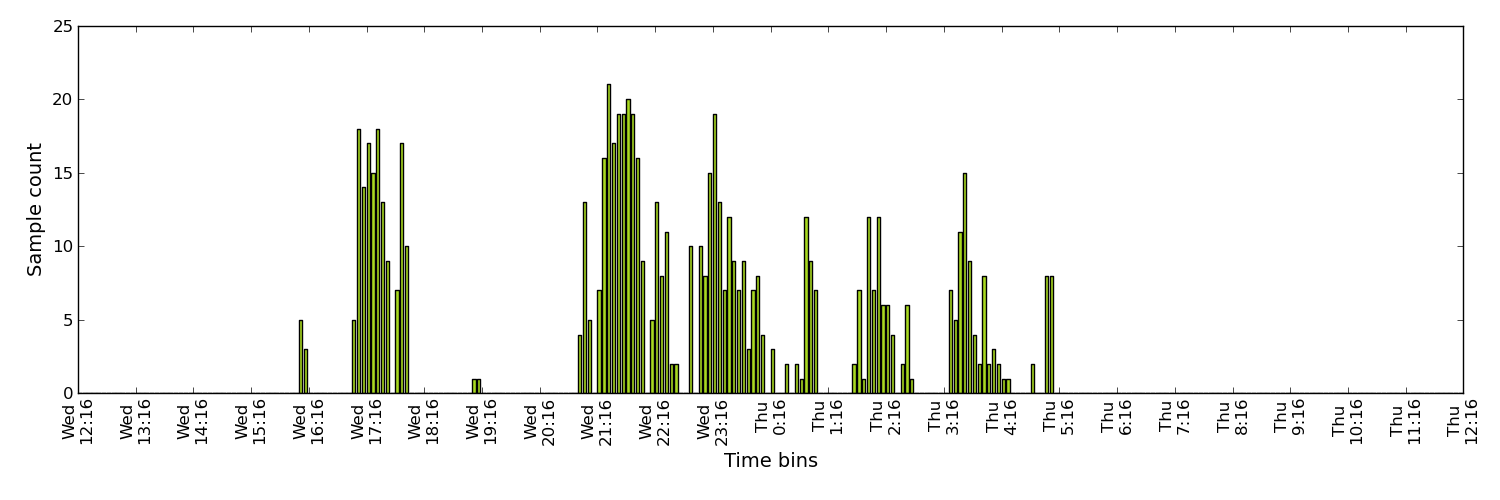
\includegraphics[width =\textwidth]{figures/combinations/ap_15188_histo.png}
\caption{Sample density of AP 15188 for userX}
\label{samples_6_2nd_day_1_A}
\end{figure}

\begin{figure}[!h]
\centering
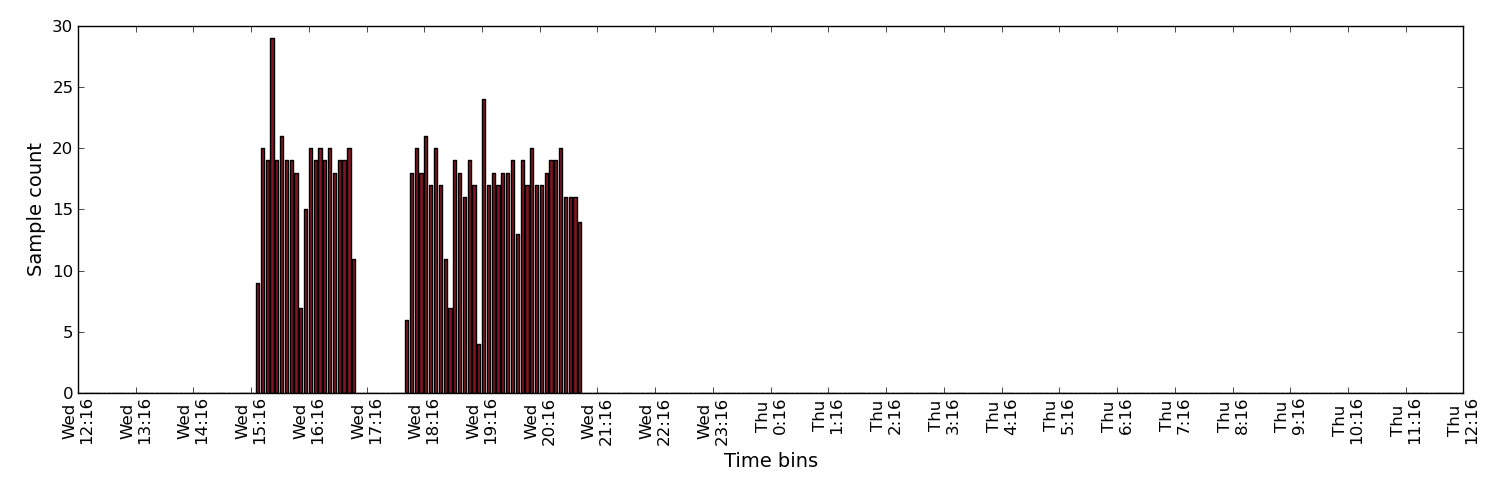
\includegraphics[width =\textwidth]{figures/combinations/ap_15190_histo.png}
\caption{Sample density of AP 15190 for userX}
\label{samples_6_2nd_day_2_A}
\end{figure}

\begin{figure}[!h]
\centering
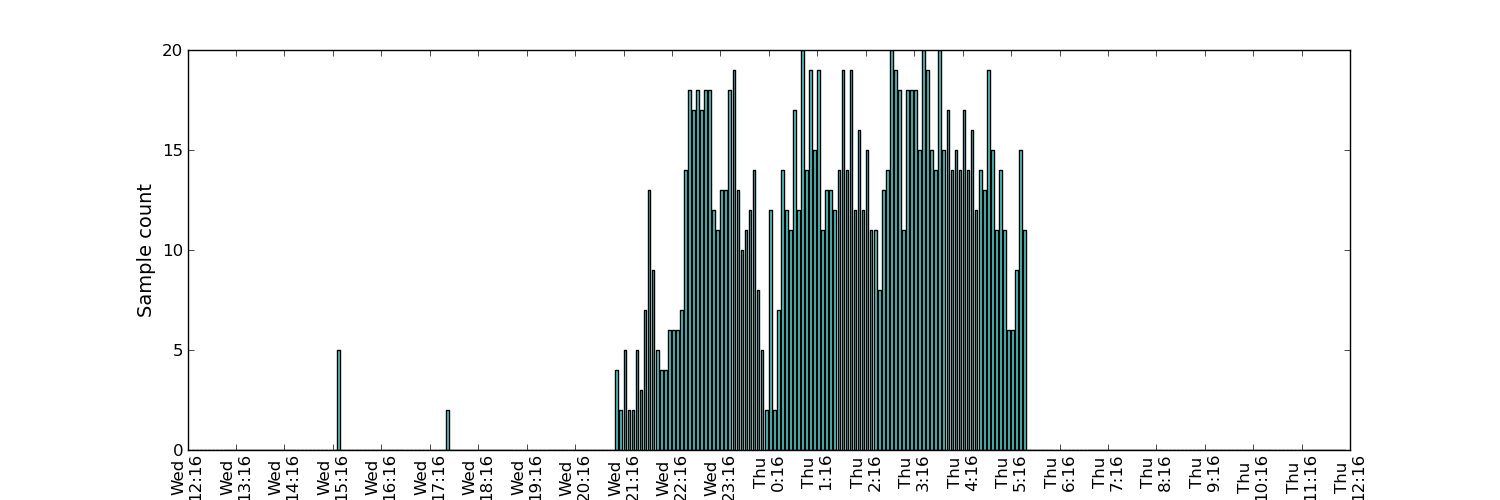
\includegraphics[width =\textwidth]{figures/combinations/ap_3144_histo.png}
\caption{Sample density of AP 3144 for userX}
\label{samples_6_2nd_day_3_A}
\end{figure}

\subsection{Average signal strength for APs identified for a user}
\label{appendix_avg_signal}

This section contains the visualization for the signal strength of APs 15188
(Fig.~\ref{avg_6_2nd_day_1_A}), 15190 (Fig.~\ref{avg_6_2nd_day_2_A}) and 3144
(Fig.~\ref{avg_6_2nd_day_3_A}) calculated for $5$ minutes time bins over the
course of one day from the data gathered for userZ.

\begin{figure}[!h]
\centering
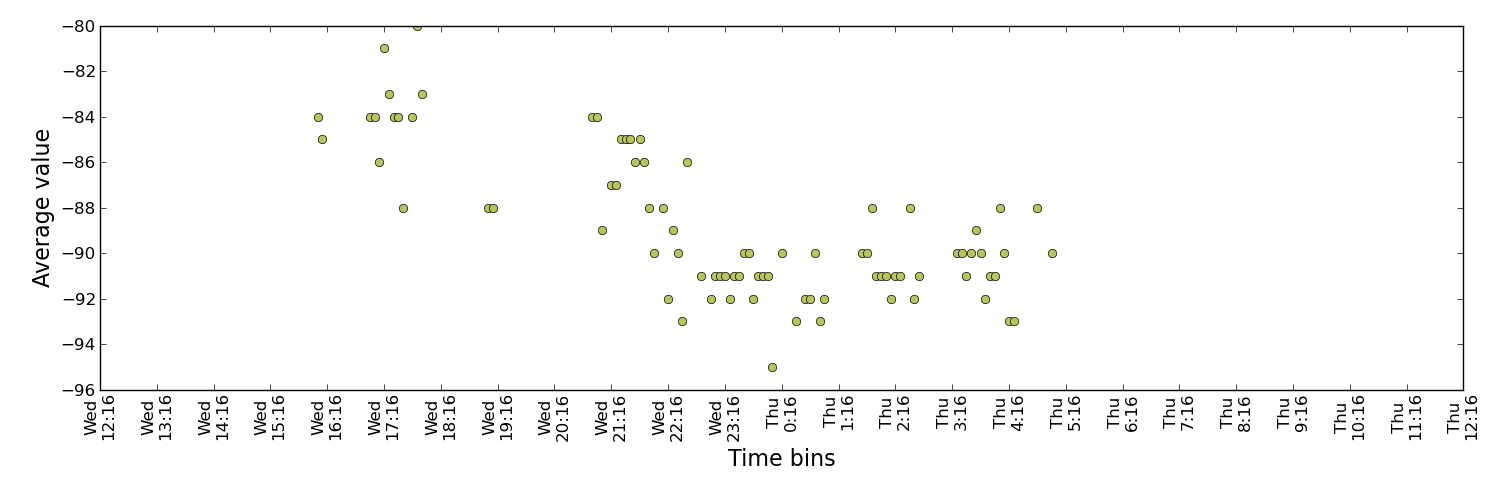
\includegraphics[width =\textwidth]{figures/combinations/user_6_sorted_1days_plot_15188_avg_sig.png}
\caption{Sample density of AP 15188 for userZ}
\label{avg_6_2nd_day_1_A}
\end{figure}

\begin{figure}[!h]
\centering
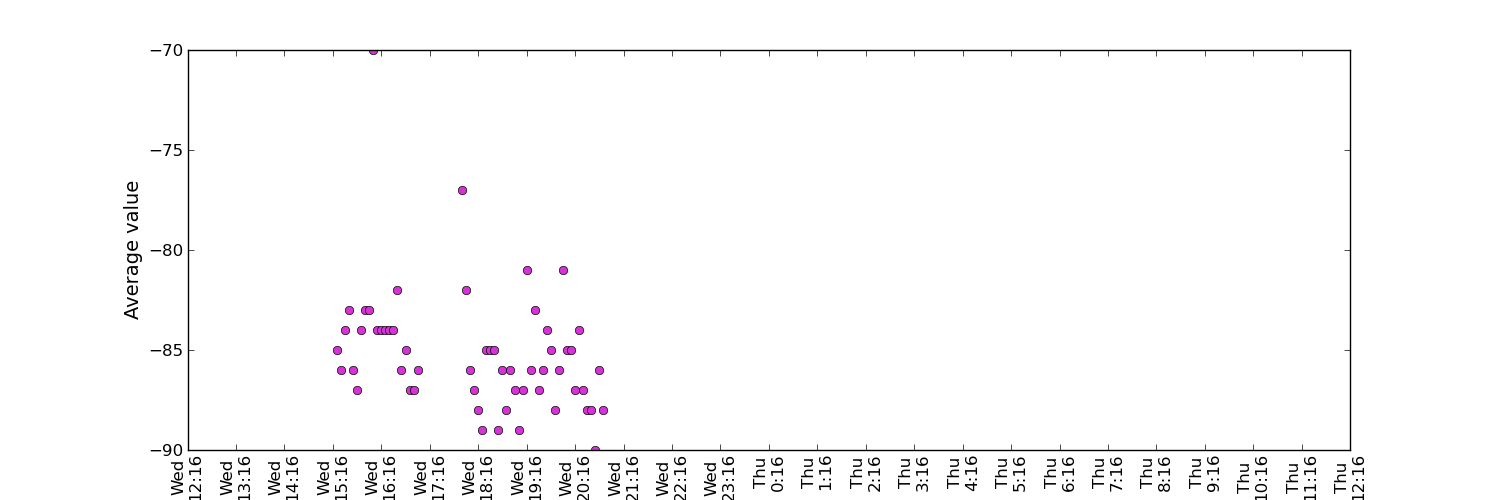
\includegraphics[width =\textwidth]{figures/combinations/user_6_sorted_1days_plot_15190_avg_sig.png}
\caption{Sample density of AP 15190 for userZ}
\label{avg_6_2nd_day_2_A}
\end{figure}

\begin{figure}[!h]
\centering
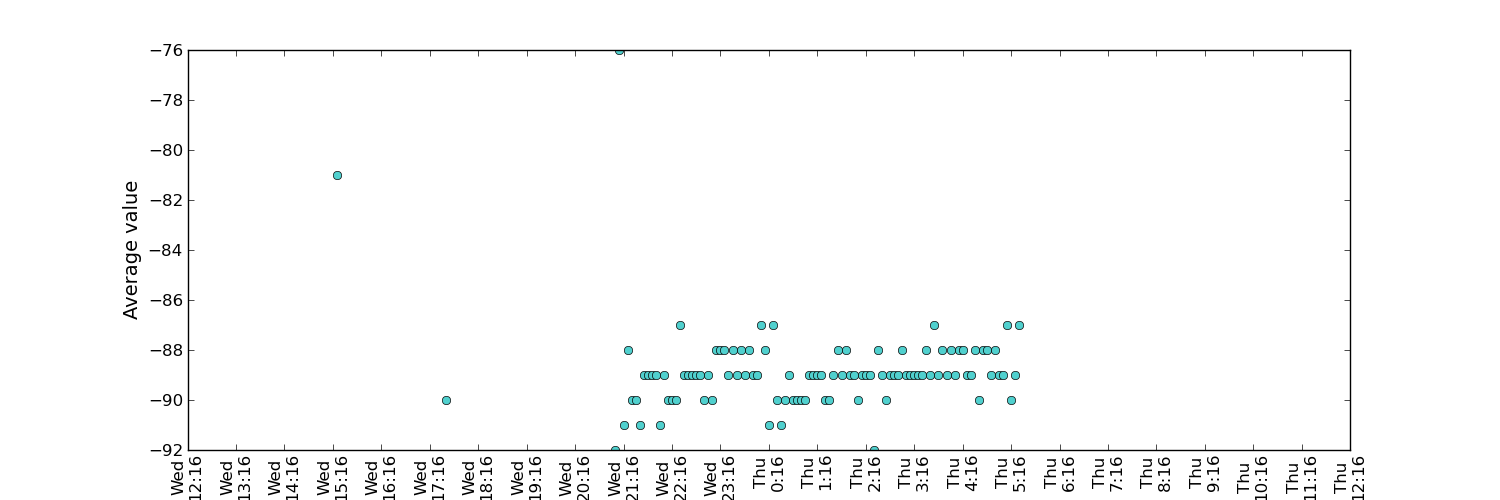
\includegraphics[width =\textwidth]{figures/combinations/user_6_sorted_1days_plot_3144_avg_sig.png}
\caption{Sample density of AP 3144}
\label{avg_6_2nd_day_3_A}
\end{figure}

\subsection{Running average signal strength}
\label{appendix_rn_avg}

This section contains the visualization for the running averages calculated for
$2$ (Fig.~\ref{user_1_AP1613_rn2avg_1d_A}), $5$
(Fig.~\ref{user_1_AP1613_rn2avg_1d_A}) and $10$
(Fig.~\ref{user_1_AP1613_rn2avg_1d_A}) minutes time bins for AP $1613$
identified in a time frame of one day (Fig.\ref{user_1_APs_1d_ap}).

\begin{figure}[!h]
\centering
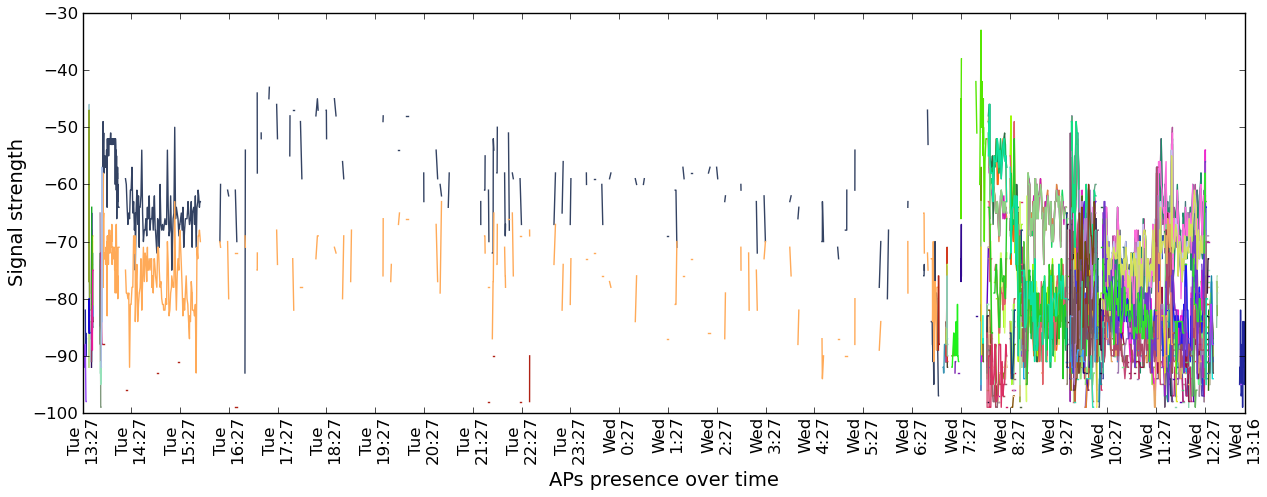
\includegraphics[width
=\textwidth]{figures/rn_avg/user_1_sorted_1days_plot.png}
\caption{Example of APs presence over time for userT}
\label{user_1_APs_1d_ap_A}
\end{figure}

\begin{figure}[!h]
\centering
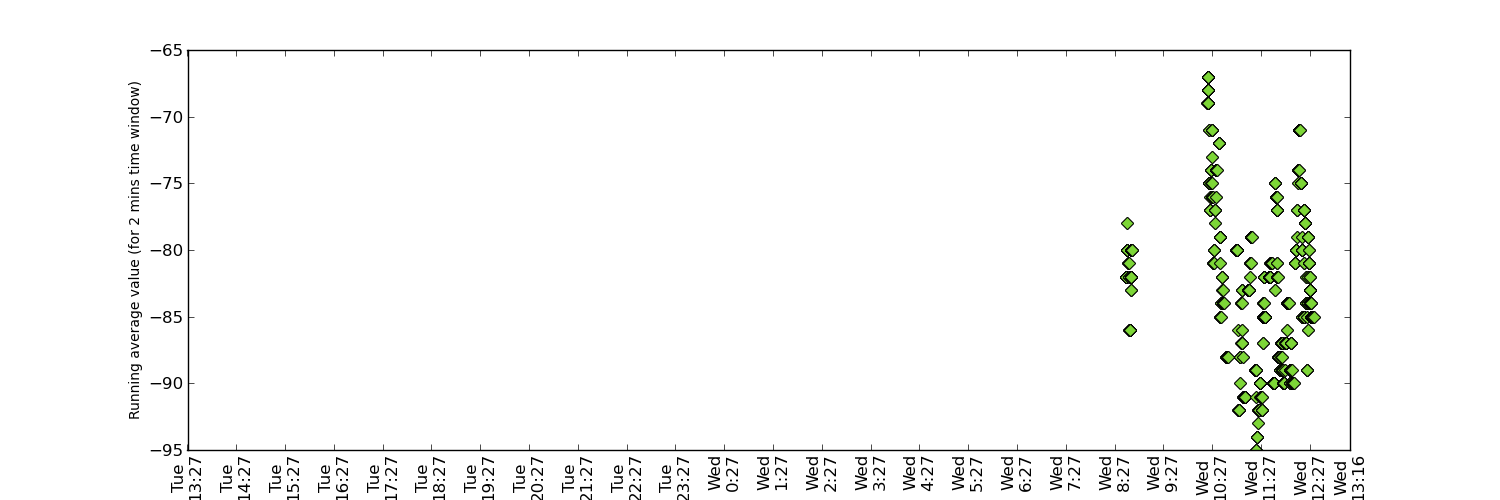
\includegraphics[width
=\textwidth]{figures/rn_avg/user_1_sorted_1days_plot_1613_rn_avg_sig_2.png}
\caption{Running average for AP 1613 for userT during 1 day (2 minute time
bins)}
\label{user_1_AP1613_rn2avg_1d_A}
\end{figure}

\begin{figure}[!h]
\centering
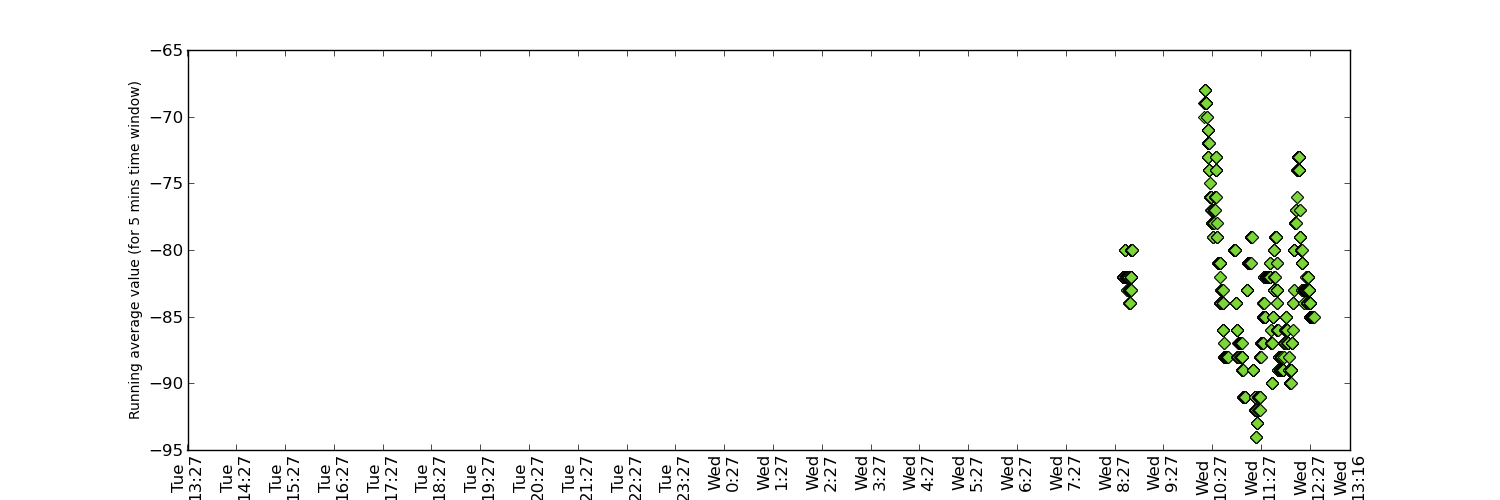
\includegraphics[width
=\textwidth]{figures/rn_avg/user_1_sorted_1days_plot_1613_rn_avg_sig_5.png}
\caption{Running average for AP 1613 for userT during 1 day (5 minute time
bins)}
\label{user_1_AP1613_rn5avg_1d_A}
\end{figure}

\begin{figure}[!h]
\centering
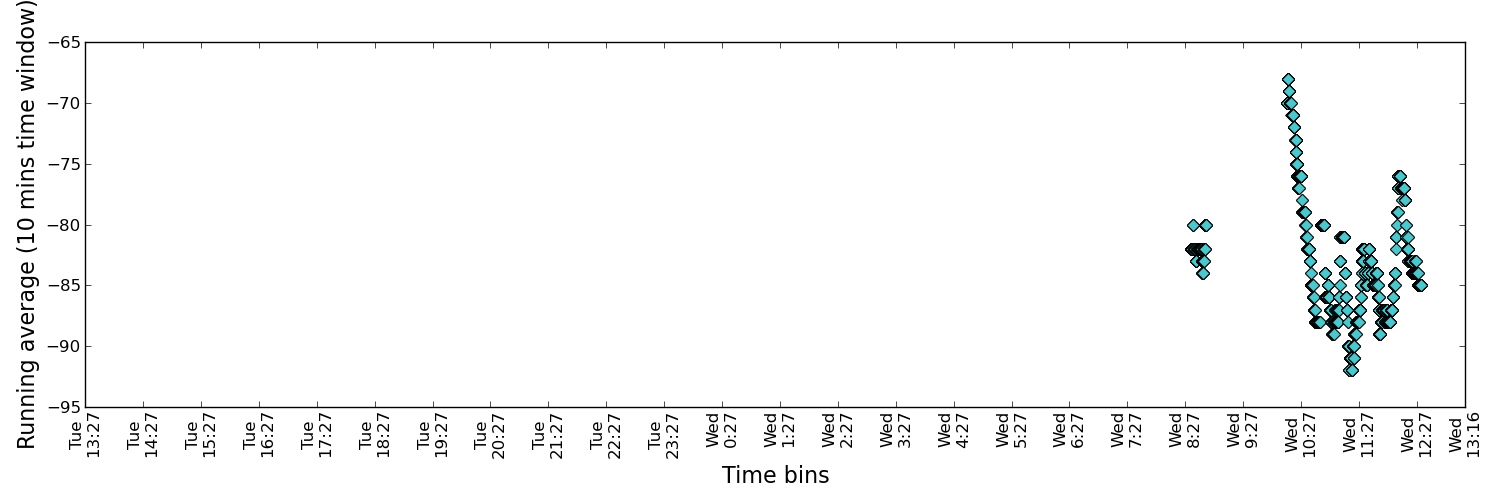
\includegraphics[width
=\textwidth]{figures/rn_avg/user_1_sorted_1days_plot_1613_rn_avg_sig_10.png}
\caption{Running average for AP 1613 for userT during 1 day (10 minute time
bins)}
\label{user_1_AP1613_rn10avg_1d_A}
\end{figure}

\subsection{Signal presence}
\label{appendix_pres}
This section contains the visualization for the presence of APs for a period of
$2$ days for an user from the SensibleDTU database
(Fig.~\ref{user_3_pres_2d_A}).The presence for APs is determined for $5$ minutes
time bins over the $2$ days.
Fig.~\ref{user_3_APs_2d_A} presents all the APs (and their signals) visualized
for the same $2$ days.

\begin{figure}[!h]
\centering
\includegraphics[width
=\textwidth]{figures/presence/user_3_sorted_2days_plot.png}
\caption{Scanned APs for an user throughout a duration of 2 days}
\label{user_3_APs_2d_A}
\end{figure}

\begin{figure}[!h]
\centering
\includegraphics[width=1\textwidth]{figures/presence/user_3_sorted_2days_no_rssi_plot.png}
\caption{The most common 50 APs for an user during 2 days (presence
visualization calculated for 5 minutes time bins)}
\label{user_3_pres_2d_A}
\end{figure}

\subsection{Locations extracted using k-means}
\label{appendix_kmeans}
                                 %Appendix A
%-----------
% Backmatter
%-----------
\backmatter
\chaptermark{Bibliography}
\renewcommand{\sectionmark}[1]{\markright{#1}}
\sectionmark{Bibliography}
\addcontentsline{toc}{chapter}{Bibliography}        %Force addition of Bibliography to TOC
\bibliographystyle{alpha}                           %Use alpha codes for references
\nocite{*}
\bibliography{References}                           %Bibliography file called
\end{document}
% % % EOF % % %